% !Mode:: "TeX:UTF-8"

\documentclass[12pt,openany,oneside]{book}

% !Mode:: "TeX:UTF-8"
% !Tex Program = xelatex
% Author: Unlucky(http://blog.thebeyond.name)
%         Myautsai(http://mckelv.in)

%%%%%%%%%% Package %%%%%%%%%%%%
\usepackage{graphicx}                       % 支持插图处理
\usepackage[a4paper,
              text={148true mm,223true mm},
			  top=37true mm,
			  bottom=37true mm,
			  left=31true mm,
			  right=31true mm,
			  head=7true mm,
			  headsep=2.5true mm,
			  foot=7true mm
			]{geometry}                      % 支持版面尺寸设置
\usepackage{titlesec}                       % 控制标题的宏包
\usepackage{titletoc}                       % 控制目录的宏包
\usepackage{fancyhdr}                       % fancyhdr宏包 支持页眉和页脚的相关定义
%\usepackage[UTF8]{ctex}
\usepackage[CJKnumber]{xeCJK}                 %xeCJK中文支持,并提供将阿拉伯数字转换成中文数字的命令
\usepackage{color}                          % 支持彩色
\usepackage{amsmath}                        % AMSLaTeX宏包 用来排出更加漂亮的公式
\usepackage{amssymb}                        % 数学符号生成命令
\usepackage[below]{placeins}                %允许上一个section的浮动图形出现在下一个section的开始部分,还提供\FloatBarrier命令,使所有未处理的浮动图形立即被处理
\usepackage{flafter}                        % 使得所有浮动体不能被放置在其浮动环境之前,以免浮动体在引述它的文本之前出现.
\usepackage{multirow}                       % 使用Multirow宏包,使得表格可以合并多个row格
\usepackage{booktabs}                       % 表格,横的粗线;\specialrule{1pt}{0pt}{0pt}
\usepackage{longtable}                      % 支持跨页的表格。
\usepackage{tabularx}                       % 自动设置表格的列宽
\usepackage{subfigure}                      % 支持子图 %centerlast 设置最后一行是否居中
\usepackage[subfigure]{ccaption}            % 支持子图的中文标题
\usepackage[sort&compress,numbers]{natbib}  % 支持引用缩写的宏包
\usepackage{enumitem}                       % 使用enumitem宏包,改变列表项的格式
\usepackage{calc}                           % 长度可以用+ - * / 进行计算
\usepackage{txfonts}                        % 字体宏包
\usepackage{bm}                             % 处理数学公式中的黑斜体的宏包
\usepackage[amsmath,thmmarks,hyperref]{ntheorem}  % 定理类环境宏包,其中 amsmath 选项用来兼容 AMS LaTeX 的宏包
%\usepackage{CJKnumb}                        % 提供将阿拉伯数字转换成中文数字的命令
\usepackage{indentfirst}                    % 首行缩进宏包
%\usepackage{CJKutf8}                        % 用在UTF8编码环境下,它可以自动调用CJK,同时针对UTF8编码作了设置。
%\usepackage{hypbmsec}                      % 用来控制书签中标题显示内容
\usepackage{CJKfntef}

\usepackage{times}
\usepackage{fontspec,xunicode,xltxtra}      % XeLaTeX相关字体字库

%如果您的pdf制作中文书签有乱码使用如下命令,就可以解决了
\usepackage[xetex, unicode,
              pdfstartview=FitH,
              CJKbookmarks=true,
              bookmarksnumbered=true,
              bookmarksopen=true,
              colorlinks=true,
			  citecolor=black,
              linkcolor=black,
              anchorcolor=black,
              urlcolor=black,
              breaklinks=true
            ]{hyperref}
 % 定义所需宏包

\begin{document}
% !Mode:: "TeX:UTF-8"
% Author: Unlucky(http://blog.thebeyond.name)
%         MCKelvin(http://mckelv.in)

%%%%%%%%%% Fonts Definition and Basics %%%%%%%%%%%%%%%%%
\XeTeXlinebreaklocale "zh"
\XeTeXlinebreakskip = 0pt plus 1pt minus 0.1pt
\setCJKfamilyfont{song}{SimSun}             % 宋体
\newcommand{\song}{\CJKfamily{song}}
\setCJKfamilyfont{fs}{FangSong}             % 仿宋体
\newcommand{\fs}{\CJKfamily{fs}}
\setCJKfamilyfont{kai}{KaiTi}               % 楷体
\newcommand{\kai}{\CJKfamily{kai}}
\setCJKfamilyfont{hei}{SimHei}              % 黑体
\newcommand{\hei}{\CJKfamily{hei}}
\setCJKfamilyfont{li}{LiSu}                 % 隶书
\newcommand{\li}{\CJKfamily{li}}
\setCJKfamilyfont{tnroman}{Times New Roman} % Times New Roman
\newcommand{\tnroman}{\CJKfamily{tnroman}}

\newcommand{\yihao}{\fontsize{26pt}{26pt}\selectfont}       % 一号, 单倍行距
\newcommand{\xiaoyi}{\fontsize{24pt}{24pt}\selectfont}      % 小一, 单倍行距
\newcommand{\erhao}{\fontsize{22pt}{22pt}\selectfont}       % 二号, 单倍行距
\newcommand{\xiaoer}{\fontsize{18pt}{18pt}\selectfont}      % 小二, 单倍行距
\newcommand{\sanhao}{\fontsize{16pt}{16pt}\selectfont}      % 三号, 单倍行距
\newcommand{\xiaosan}{\fontsize{15pt}{22.5pt}\selectfont}   % 小三, 1.5倍行距
\newcommand{\sihao}{\fontsize{14pt}{14pt}\selectfont}       % 四号, 单倍行距
\newcommand{\xiaosi}{\fontsize{12pt}{18pt}\selectfont}      % 小四, 1.5倍行距
\newcommand{\wuhao}{\fontsize{10.5pt}{10.5pt}\selectfont}   % 五号, 单倍行距
\newcommand{\xiaowu}{\fontsize{9pt}{9pt}\selectfont}        % 小五, 单倍行距

\setmainfont{Times New Roman}
\setCJKmainfont{SimSun}
\setCJKmonofont{SimSun}

% \CJKcaption{gb_452}
% \CJKtilde  % 重新定义了波浪符~的意义
\newcommand\prechaptername{第}
\newcommand\postchaptername{章}

% \punctstyle{plain}
% 调整罗列环境的布局
\setitemize{leftmargin=3em,itemsep=0em,partopsep=0em,parsep=0em,topsep=-0em}
\setenumerate{leftmargin=3em,itemsep=0em,partopsep=0em,parsep=0em,topsep=0em}
% \setlength{\baselineskip}{20pt}
% \renewcommand{\baselinestretch}{1.38} % 设置行距

% 避免宏包 hyperref 和 arydshln 不兼容带来的目录链接失效的问题。
\def\temp{\relax}
\let\temp\addcontentsline
\gdef\addcontentsline{\phantomsection\temp}

% 自定义项目列表标签及格式 \begin{publist} 列表项 \end{publist}
\newcounter{pubctr} %自定义新计数器
\newenvironment{publist}{%%%%%定义新环境
  \begin{list}{[\arabic{pubctr}]} %%标签格式
    {
      \usecounter{pubctr}
      \setlength{\leftmargin}{2.5em}   % 左边界 \leftmargin =\itemindent + \labelwidth + \labelsep
      \setlength{\itemindent}{0em}     % 标号缩进量
      \setlength{\labelsep}{1em}       % 标号和列表项之间的距离,默认0.5em
      \setlength{\rightmargin}{0em}    % 右边界
      \setlength{\topsep}{0ex}         % 列表到上下文的垂直距离
      \setlength{\parsep}{0ex}         % 段落间距
      \setlength{\itemsep}{0ex}        % 标签间距
      \setlength{\listparindent}{0pt}  % 段落缩进量
    }}
  {\end{list}}%%%%%

\makeatletter
\renewcommand\normalsize{
  \@setfontsize\normalsize{12pt}{18pt} % 小四对应12pt,1.5倍行距对应18pt
  \setlength\abovedisplayskip{4pt}
  \setlength\abovedisplayshortskip{4pt}
  \setlength\belowdisplayskip{\abovedisplayskip}
  \setlength\belowdisplayshortskip{\abovedisplayshortskip}
  \let\@listi\@listI}
\def\defaultfont{\renewcommand{\baselinestretch}{1.35}\normalsize\selectfont} %Word和XeLaTeX行距的缩放因子,Word偏小,该值为实验值,可根据实际情况做修改
% 设置行距和段落间垂直距离
\renewcommand{\CJKglue}{\hskip 0.96pt plus 0.08\baselineskip} %加大字间距,使每行33个字

\makeatother
%%%%%%%%%%%%% Contents %%%%%%%%%%%%%%%%%
% 主目录设置
\renewcommand{\contentsname}{目\qquad 录}
\setcounter{tocdepth}{1}
% Chapter目录设置
\titlecontents{chapter}[2em]{\vspace{.5\baselineskip}\wuhao\hei}
{\prechaptername\CJKnumber{\thecontentslabel}\postchaptername\qquad}{}
{\hspace{.5em}\titlerule*[10pt]{$\cdot$}\wuhao\contentspage}
% Section目录设置
\titlecontents{section}[3em]{\vspace{.25\baselineskip}\wuhao\song}
{\thecontentslabel\quad}{}
{\hspace{.5em}\titlerule*[10pt]{$\cdot$}\wuhao\contentspage}
% Subsection目录设置
\titlecontents{subsection}[4em]{\vspace{.25\baselineskip}\wuhao\song}
{\thecontentslabel\quad}{}
{\hspace{.5em}\titlerule*[10pt]{$\cdot$}\wuhao\contentspage}

% 图目录设置
\renewcommand{\listfigurename}{图目录}
\newcommand{\loflabel}{图}
\renewcommand{\numberline}[1]{\loflabel~#1\hspace*{1em}}

% 表目录设置
\renewcommand{\listtablename}{表目录}
\newcommand{\lotlabel}{表}
\renewcommand{\numberline}[1]{\lotlabel~#1\hspace*{1em}}


%%%%%%%%%% Chapter and Section %%%%%%%%%%%%%%%%%
\setcounter{secnumdepth}{4}
\setlength{\parindent}{2em}
\renewcommand{\chaptername}{\prechaptername\CJKnumber{\thechapter}\postchaptername}
\titleformat{\chapter}{\centering\hei\xiaoer\bfseries}{\chaptername}{2em}{}
\titlespacing{\chapter}{0pt}{0.3\baselineskip}{1\baselineskip}
\titleformat{\section}{\hei\xiaosan\bfseries}{\thesection}{1em}{}
\titlespacing{\section}{0pt}{0.2\baselineskip}{0.5\baselineskip}
\titleformat{\subsection}{\hei\sihao\bfseries}{\thesubsection}{1em}{}
\titlespacing{\subsection}{0pt}{0.1\baselineskip}{0.3\baselineskip}
\titleformat{\subsubsection}{\xiaosan\bfseries}{\thesubsubsection}{1em}{}
\titlespacing{\subsubsection}{0pt}{0}{0}

%%%%%%%%%% Table, Figure and Equation %%%%%%%%%%%%%%%%%
\renewcommand{\tablename}{表} % 插表题头
\renewcommand{\figurename}{图} % 插图题头
\renewcommand{\thefigure}{\arabic{chapter}-\arabic{figure}} % 使图编号为 7-1 的格式 %\protect{~}
\renewcommand{\thesubfigure}{\alph{subfigure})}%使子图编号为 a)的格式
\renewcommand{\thesubtable}{(\alph{subtable})} %使子表编号为 a)的格式
\renewcommand{\thetable}{\arabic{chapter}-\arabic{table}}%使表编号为 7-1 的格式
\renewcommand{\theequation}{\arabic{chapter}-\arabic{equation}}%使公式编号为 7-1 的格式

%% 定制浮动图形和表格标题样式
\makeatletter
\long\def\@makecaption#1#2{%
  \vskip\abovecaptionskip
  \sbox\@tempboxa{\centering\wuhao\song{#1\qquad #2} }%
  \ifdim \wd\@tempboxa >\hsize
  \centering\wuhao\song{#1\qquad #2} \par
  \else
  \global \@minipagefalse
  \hb@xt@\hsize{\hfil\box\@tempboxa\hfil}%
  \fi
  \vskip\belowcaptionskip}
\makeatother
\captiondelim{~~~~} %用来控制longtable表头分隔符

%%%%%%%%%% Theorem Environment %%%%%%%%%%%%%%%%%
\theoremstyle{plain}
\theorembodyfont{\song\rmfamily}
\theoremheaderfont{\hei\rmfamily}
\newtheorem{theorem}{定理~}[chapter]
\newtheorem{lemma}{引理~}[chapter]
\newtheorem{axiom}{公理~}[chapter]
\newtheorem{proposition}{命题~}[chapter]
\newtheorem{corollary}{推论~}[chapter]
\newtheorem{definition}{定义~}[chapter]
\newtheorem{conjecture}{猜想~}[chapter]
\newtheorem{example}{例~}[chapter]
\newtheorem{remark}{注~}[chapter]
\newtheorem{algorithm}{算法~}[chapter]
\newenvironment{proof}{\noindent{\hei 证明:}}{\hfill $ \square $ \vskip 4mm}
\theoremsymbol{$\square$}

%%%%%%%%%% Page: number, header and footer  %%%%%%%%%%%%%%%%%

% \frontmatter 或 \pagenumbering{roman}
% \mainmatter 或 \pagenumbering{arabic}
\makeatletter
\renewcommand\frontmatter{\clearpage
  \@mainmatterfalse
  \pagenumbering{Roman}} % 正文前罗马字体编号
\makeatother


%%%%%%%%%% References %%%%%%%%%%%%%%%%%
\renewcommand{\bibname}{参考文献}
% 重定义参考文献样式,来自thu
\makeatletter
\renewenvironment{thebibliography}[1]{%
  \titleformat{\chapter}{\raggedright\sihao\hei}{\chaptername}{2em}{}
  \chapter*{\bibname}%
  \wuhao
  \list{\@biblabel{\@arabic\c@enumiv}}%
  {\renewcommand{\makelabel}[1]{##1\hfill}
    \settowidth\labelwidth{0.5cm}
    \setlength{\labelsep}{0pt}
    \setlength{\itemindent}{0pt}
    \setlength{\leftmargin}{\labelwidth+\labelsep}
    \addtolength{\itemsep}{-0.7em}
    \usecounter{enumiv}%
    \let\p@enumiv\@empty
    \renewcommand\theenumiv{\@arabic\c@enumiv}}%
  \sloppy\frenchspacing
  \clubpenalty4000%
  \@clubpenalty \clubpenalty
  \widowpenalty4000%
  \interlinepenalty4000%
  \sfcode`\.\@m}
{\def\@noitemerr
  {\@latex@warning{Empty `thebibliography' environment}}%
  \endlist\frenchspacing}
\makeatother

\addtolength{\bibsep}{-0.5em} % 缩小参考文献间的垂直间距
\setlength{\bibhang}{2em} %每个条目自第二行起缩进的距离

% 参考文献引用作为上标出现
% \newcommand{\citeup}[1]{\textsuperscript{\cite{#1}}}
\makeatletter
\def\@cite#1#2{\textsuperscript{[{#1\if@tempswa , #2\fi}]}}
\makeatother
%% 引用格式
\bibpunct{[}{]}{,}{s}{}{,}

%%%%%%%%%% Cover %%%%%%%%%%%%%%%%%
% 封面、摘要、版权、致谢格式定义
\makeatletter
\def\ctitle#1{\def\@ctitle{#1}}\def\@ctitle{}
\def\caffil#1{\def\@caffil{#1}}\def\@caffil{}
\def\csubject#1{\def\@csubject{#1}}\def\@csubject{}
\def\cauthor#1{\def\@cauthor{#1}}\def\@cauthor{}
\def\csupervisor#1{\def\@csupervisor{#1}}\def\@csupervisor{}
\def\cdate#1{\def\@cdate{#1}}\def\@cdate{}
\long\def\cabstract#1{\long\def\@cabstract{#1}}\long\def\@cabstract{}
\long\def\eabstract#1{\long\def\@eabstract{#1}}\long\def\@eabstract{}
\def\ckeywords#1{\def\@ckeywords{#1}}\def\@ckeywords{}
\def\ekeywords#1{\def\@ekeywords{#1}}\def\@ekeywords{}
\def\cheading#1{\def\@cheading{#1}}\def\@cheading{}

% 在book文件类别下,\leftmark自动存录各章之章名,\rightmark记录节标题
\pagestyle{fancy}
% 去掉章节标题中的数字 务必放到\pagestyle{fancy}之后才会起作用
%% 不要注销这一行,否则页眉会变成:“第1章1  绪论”样式
\renewcommand{\chaptermark}[1]{\markboth{\chaptername~\ #1}{}}
\fancyhf{}
% \fancyhead[C]{\song\wuhao \leftmark} % 页眉显示章节名称
\fancyhead[C]{\song\xiaowu \@cheading}
% \fancyhead[CO]{\song\wuhao \@cheading}
% \fancyhead[CE]{\song\wuhao \@cheading}
\fancyfoot[C]{\song\xiaowu ~\thepage~}

\fancypagestyle{plain}{% 设置开章页页眉页脚风格
  \fancyhf{}%
  % \fancyhead[C]{\song\wuhao \leftmark}
  \fancyhead[C]{\song\xiaowu \@cheading}
  \fancyfoot[C]{\song\xiaowu ~\thepage~ } %%首页页脚格式
  \renewcommand{\headrulewidth}{0.5pt}%
  \renewcommand{\footrulewidth}{0pt}%
}

% 定义封面
\def\makecover{
  % \cleardoublepage%
  \phantomsection
  \pdfbookmark[-1]{\@ctitle}{ctitle}

  \begin{titlepage}
  	\vspace*{-2.5mm}
    \begin{center}
      %校名
      \begin{figure}[h]
        \centering
        
\includegraphics[width=9.84cm]{figures/zjut}
      \end{figure}
      \vspace*{9.66mm}
	  \song\yihao{本科毕业设计说明书(论文)}\\
	  \vspace*{10.0mm}
	  \hei\xiaoer{(2013届)}\\
      \vspace*{8.5mm}
      %校徽
      \begin{figure}[h]
        \centering
        
\includegraphics[width=2.73cm]{figures/zjutlogo}
      \end{figure}
      \vspace*{0.0mm}
      \renewcommand{\arraystretch}{1.0}
      \begin{tabular}{lc}
        \song\erhao{论文题目\quad} & \song\xiaoer{\@ctitle} \\ \cline{2-2}
      \end{tabular}\\
	  \vspace*{11.1mm}
      \setlength{\arrayrulewidth}{0.5pt}
      {\song\sihao
        \renewcommand{\arraystretch}{2.0}
        \begin{tabular}{lc}
          作者姓名\qquad &  \@cauthor \\ \cline{2-2}
          指导教师\qquad &  \@csupervisor \\ \cline{2-2}
          \\
          学科(专业)\qquad &  \@csubject \\ \cline{2-2}
          所在学院\qquad &  \@caffil \\ \cline{2-2}\cline{2-2}
          提交日期\qquad & \@cdate \\ \cline{2-2}
        \end{tabular}
	  }
    \end{center}
  \end{titlepage}

  %%%%%%%%%%%%%%%%%%% Abstract and Keywords  %%%%%%%%%%%%%%%%%%%%%%%
  \clearpage
  \markboth{摘~要}{摘~要}
  \addcontentsline{toc}{chapter}{摘~要}
  \setlength{\parskip}{24pt}
  \chapter*{\centering\hei\xiaoer{摘\qquad 要}}
  \setlength{\parskip}{18pt}
  \setcounter{page}{1}
  %\song\defaultfont
  \setlength{\parskip}{0pt}
  \song\xiaosi{\@cabstract}
  \vspace{15pt}

  \hangafter=1\hangindent=52.3pt\noindent
  \hei\xiaosi{关键词:} \song\xiaosi{\@ckeywords}

  %%%%%%%%%%%%%%%%%%% English Abstract  %%%%%%%%%%%%%%%%%%%%%%%%%%%%%%
  \clearpage
  % \phantomsection
  \markboth{ABSTRACT}{ABSTRACT}
  \addcontentsline{toc}{chapter}{ABSTRACT}
  \setlength{\parskip}{24pt}
  \chapter*{\centering\tnroman\xiaoer\textbf{ABSTRACT}}
  \setlength{\parskip}{18pt}
  % \vspace{\baselineskip}
  \setlength{\parskip}{0pt}
  \@eabstract
  \vspace{15pt}

  \hangafter=1\hangindent=60pt\noindent
  {\tnroman\xiaosi\textbf{Keywords:}}  {\tnroman\xiaosi{\@ekeywords}}
}
\makeatother  % 格式设置
\graphicspath{{figures/}}  % 定义所有的eps文件在 figures 子目录下
% !Mode:: "TeX:UTF-8"
%%============================================================
%% 中文封面
\thispagestyle{empty}
\pdfbookmark[-1]{\zjuttitlec}{zjutreportcover}
\phantomsection \label{zjutreportcover}
\vspace*{-2.5mm}
% 校名
\begin{center}
   
\includegraphics[width=98.40mm]{figures/zjut}
\end{center}
\vspace*{9.66mm}
\centerline{\songti\yihao{\reporttitle}}
\vspace*{10.0mm}
\centerline{\heiti\xiaoer\textbf{(\zjutgrade\ 届)}}
\vspace*{8.5mm}
% 校徽
\begin{center}
  
\includegraphics[width=27.3mm]{figures/zjutlogo}
\end{center}

\vspace*{0.0mm}
\renewcommand{\arraystretch}{1.0}
\hspace*{7.4mm}
{\songti\erhao{论文题目}}
\hspace{6mm}
\begin{minipage}[t]{95mm}
    \linespread{1.1}{\songti\xiaoer\uline{\zjuttitlec}}
\end{minipage}
\vspace*{9mm}
\begin{center}
    \setlength{\arrayrulewidth}{0.5pt}
    {\songti\sihao
        \renewcommand{\arraystretch}{1.4}
        \begin{tabular}{lc}
            作者姓名 \qquad &  \zjutauthornamec \\ \cline{2-2}
            指导教师\qquad &  \zjutmentorc\\ \cline{2-2}
            \\
            学科(专业)\qquad &  \zjutmajor \\ \cline{2-2}
            所在学院\qquad &  \zjutcollegec \\ \cline{2-2}\cline{2-2}
            提交日期\qquad & \zjutsubmitteddatee \\ \cline{2-2}
        \end{tabular}
    }
\end{center}

  % 封面

\mainmatter\defaultfont\sloppy\raggedbottom

\begingroup % 在组内的chapter不换行
\let\clearpage\relax % chapter之后不换页
%%%%%%%%%% 摘要 %%%%%%%%%%
\titleformat{\chapter}{\centering\hei\sanhao\bfseries}{\chaptername}{1em}{} % 标题居中,黑体三号
% !Mode:: "TeX:UTF-8"

\chapter*{浙江工业大学本科生毕业设计外文翻译模板}
\noindent{\hei\bfseries 摘要:}摘要是论文内容的高度概括,应具有独立性和自含性,即不阅读论文的全文,就能获得必要的信息。
摘要应包括本论文的目的、主要研究内容、研究方法、创造性成果及其理论与实际意义。
摘要中不宜使用公式、化学结构式、图表和非公知公用的符号和术语,不标注引用文献编号。避免将摘要写成目录式的内容介绍。\\
{\hei\bfseries 关键词:}关键词~1;关键词~2;关键词~3;……;关键词~6(关键词总共~3~—~6~个,最后一个关键词后面没有标点符号)
%关键词~1;关键词~2;关键词~3;……;关键词~6(关键词总共~3~—~6~个,最后一个关键词后面没有标点符号)

\newline
\titleformat{\chapter}{\hei\sihao\bfseries}{\chaptername}{1em}{} % 恢复标题居左,黑体四号

%%%%%%%%%% 正文 %%%%%%%%%%
% !Mode:: "TeX:UTF-8"

\chapter{模板介绍与注意事项}
\section{模板说明}

ZJUTThesis~是为了帮助浙江工业大学本科毕业生撰写毕业论文而编写的~\XeLaTeX~论文模板,其前提是用户已经能处理一般的~\XeLaTeX~文档,并对~BibTeX~有一定了解,如果你从来没有接触过~\XeLaTeX~,建议先学习相关基础知识,磨刀不误砍柴工,能有助你更好使用模板\cite{huwei}。

由于作者水平有限,虽然现在的这个版本基本上满足了学校的要求,但难免存在不足之处,欢迎大家积极反馈,更希望浙江工业大学~\XeLaTeX~爱好者能一同完善此模板,让更多同学受益。

如有模板的疑问或有意向加入模板的维护和编写队伍中来,请给作者: Unlucky(unlucky1990@gmail.com)或MCKelvin(ibmmc@live.com)写信。

\section{下载安装}
ZJUTThesis~主页:~\url{https://github.com/unlucky/zjutthesis}。除此之外,不再维护任何镜像。

\section{目录内容}
本~\XeLaTeX~模板的源文件即为本科毕业设计论文中使用的模板,用户可以通过修改这些文件来编辑自己的毕业论文。
\begin{itemize}
\item{zjutmain.tex}:主文件,包含封面部分和其他章节的引用信息。
\item{preface}: 包含本科毕业设计论文的封面和中英文摘要。
\item{body}: 包含本文正文中的所有章节。
\begin{itemize}
\item{intros.tex}: 包括本~\XeLaTeX~模板的介绍,编译方法和使用方法。
\item{figures.tex}: 包含论文中图片的插入和引用方法。
\item{tables.tex}: 包含论文中表格的插入和引用方法。
\item{equations.tex}: 包含论文中数学符号、公式的书写和排版方法。
\item{others.tex}: 包含论文中使用的罗列环境,定理环境等其他环境的排版方法。
\item{conclusion.tex}: 包含本文的总结。
\end{itemize}
\item{appendix}:存放论文的外文资料,中文译文和致谢部分。
\item{references/reference.bib}:存放论文所引用的全部参考文献信息。
\item{make.bat/Makefile}:Windows/Linux环境下的编译脚本
\item{clean.bat}:双击此文件,可以用来清理~ZJUTmain.tex~在编译之后生成的所有附属文件,如后缀名为~.aux~,~.log~,~.bak~的文件。
\end{itemize}

需要说明的是,以上文件名并不是固定的,各位同学可以新建一个~tex~文件,例如~algorithm.tex,放在~body~目录下,并且在~zjutmain.tex~中调用:
\begin{verbatim}
    \include{body/algorithm.tex}
\end{verbatim}
来引用之。当然你也可以重命名这些文件,只要~include~中的文件名是存在且合法,~\XeLaTeX~总能找到这些文件的。

在你写作某一章节的时候,你可能需要随时预览排版效果并~Debug,这时你可以在其他章节的\verb|\include|命令前加上一个\%,这代表注释掉本行,例如:
\begin{verbatim}
%%%%%%%%%%%%%%%%%%%%%%%%%%%%%%%%
           正文部分
%%%%%%%%%%%%%%%%%%%%%%%%%%%%%%%%
\mainmatter
% !Mode:: "TeX:UTF-8"

\chapter{模板介绍与注意事项}
\section{模板说明}

ZJUTThesis~是为了帮助浙江工业大学本科毕业生撰写毕业论文而编写的~\XeLaTeX~论文模板,其前提是用户已经能处理一般的~\XeLaTeX~文档,并对~BibTeX~有一定了解,如果你从来没有接触过~\XeLaTeX~,建议先学习相关基础知识,磨刀不误砍柴工,能有助你更好使用模板\cite{huwei}。

由于作者水平有限,虽然现在的这个版本基本上满足了学校的要求,但难免存在不足之处,欢迎大家积极反馈,更希望浙江工业大学~\XeLaTeX~爱好者能一同完善此模板,让更多同学受益。

如有模板的疑问或有意向加入模板的维护和编写队伍中来,请给作者: Unlucky(unlucky1990@gmail.com)或MCKelvin(ibmmc@live.com)写信。

\section{下载安装}
ZJUTThesis~主页:~\url{https://github.com/unlucky/zjutthesis}。除此之外,不再维护任何镜像。

\section{目录内容}
本~\XeLaTeX~模板的源文件即为本科毕业设计论文中使用的模板,用户可以通过修改这些文件来编辑自己的毕业论文。
\begin{itemize}
\item{zjutmain.tex}:主文件,包含封面部分和其他章节的引用信息。
\item{preface}: 包含本科毕业设计论文的封面和中英文摘要。
\item{body}: 包含本文正文中的所有章节。
\begin{itemize}
\item{intros.tex}: 包括本~\XeLaTeX~模板的介绍,编译方法和使用方法。
\item{figures.tex}: 包含论文中图片的插入和引用方法。
\item{tables.tex}: 包含论文中表格的插入和引用方法。
\item{equations.tex}: 包含论文中数学符号、公式的书写和排版方法。
\item{others.tex}: 包含论文中使用的罗列环境,定理环境等其他环境的排版方法。
\item{conclusion.tex}: 包含本文的总结。
\end{itemize}
\item{appendix}:存放论文的外文资料,中文译文和致谢部分。
\item{references/reference.bib}:存放论文所引用的全部参考文献信息。
\item{make.bat/Makefile}:Windows/Linux环境下的编译脚本
\item{clean.bat}:双击此文件,可以用来清理~ZJUTmain.tex~在编译之后生成的所有附属文件,如后缀名为~.aux~,~.log~,~.bak~的文件。
\end{itemize}

需要说明的是,以上文件名并不是固定的,各位同学可以新建一个~tex~文件,例如~algorithm.tex,放在~body~目录下,并且在~zjutmain.tex~中调用:
\begin{verbatim}
    \include{body/algorithm.tex}
\end{verbatim}
来引用之。当然你也可以重命名这些文件,只要~include~中的文件名是存在且合法,~\XeLaTeX~总能找到这些文件的。

在你写作某一章节的时候,你可能需要随时预览排版效果并~Debug,这时你可以在其他章节的\verb|\include|命令前加上一个\%,这代表注释掉本行,例如:
\begin{verbatim}
%%%%%%%%%%%%%%%%%%%%%%%%%%%%%%%%
           正文部分
%%%%%%%%%%%%%%%%%%%%%%%%%%%%%%%%
\mainmatter
% !Mode:: "TeX:UTF-8"

\chapter{模板介绍与注意事项}
\section{模板说明}

ZJUTThesis~是为了帮助浙江工业大学本科毕业生撰写毕业论文而编写的~\XeLaTeX~论文模板,其前提是用户已经能处理一般的~\XeLaTeX~文档,并对~BibTeX~有一定了解,如果你从来没有接触过~\XeLaTeX~,建议先学习相关基础知识,磨刀不误砍柴工,能有助你更好使用模板\cite{huwei}。

由于作者水平有限,虽然现在的这个版本基本上满足了学校的要求,但难免存在不足之处,欢迎大家积极反馈,更希望浙江工业大学~\XeLaTeX~爱好者能一同完善此模板,让更多同学受益。

如有模板的疑问或有意向加入模板的维护和编写队伍中来,请给作者: Unlucky(unlucky1990@gmail.com)或MCKelvin(ibmmc@live.com)写信。

\section{下载安装}
ZJUTThesis~主页:~\url{https://github.com/unlucky/zjutthesis}。除此之外,不再维护任何镜像。

\section{目录内容}
本~\XeLaTeX~模板的源文件即为本科毕业设计论文中使用的模板,用户可以通过修改这些文件来编辑自己的毕业论文。
\begin{itemize}
\item{zjutmain.tex}:主文件,包含封面部分和其他章节的引用信息。
\item{preface}: 包含本科毕业设计论文的封面和中英文摘要。
\item{body}: 包含本文正文中的所有章节。
\begin{itemize}
\item{intros.tex}: 包括本~\XeLaTeX~模板的介绍,编译方法和使用方法。
\item{figures.tex}: 包含论文中图片的插入和引用方法。
\item{tables.tex}: 包含论文中表格的插入和引用方法。
\item{equations.tex}: 包含论文中数学符号、公式的书写和排版方法。
\item{others.tex}: 包含论文中使用的罗列环境,定理环境等其他环境的排版方法。
\item{conclusion.tex}: 包含本文的总结。
\end{itemize}
\item{appendix}:存放论文的外文资料,中文译文和致谢部分。
\item{references/reference.bib}:存放论文所引用的全部参考文献信息。
\item{make.bat/Makefile}:Windows/Linux环境下的编译脚本
\item{clean.bat}:双击此文件,可以用来清理~ZJUTmain.tex~在编译之后生成的所有附属文件,如后缀名为~.aux~,~.log~,~.bak~的文件。
\end{itemize}

需要说明的是,以上文件名并不是固定的,各位同学可以新建一个~tex~文件,例如~algorithm.tex,放在~body~目录下,并且在~zjutmain.tex~中调用:
\begin{verbatim}
    \include{body/algorithm.tex}
\end{verbatim}
来引用之。当然你也可以重命名这些文件,只要~include~中的文件名是存在且合法,~\XeLaTeX~总能找到这些文件的。

在你写作某一章节的时候,你可能需要随时预览排版效果并~Debug,这时你可以在其他章节的\verb|\include|命令前加上一个\%,这代表注释掉本行,例如:
\begin{verbatim}
%%%%%%%%%%%%%%%%%%%%%%%%%%%%%%%%
           正文部分
%%%%%%%%%%%%%%%%%%%%%%%%%%%%%%%%
\mainmatter
\include{body/intros}
%%\include{body/figures}
%%\include{body/tables}
%%\include{body/equations}
%%\include{body/others}
%%\include{body/conclusion}
\end{verbatim}
那么,编译的时候就只编译未加~\%~的一章,在这个例子中,即本章~intros。

理论上,并不一定要把每章放在不同的文件中。但是这种自顶向下,分章节写作、编译的方法有利于提高效率,大大减少~Debug~过程中的编译时间,同时减小风险。

\section{参考文献生成方法}

\LaTeX~具有插入参考文献的能力。Google Scholar~网站上存在兼容~BibTeX~的参考文献信息,通过以下几个步骤,可以轻松完成参考文献的生成。
\begin{itemize}
  \item 在\href{http://scholar.google.com/}{谷歌学术搜索}中,
        点击\href{http://scholar.google.com/scholar_preferences?hl=en&as_sdt=0,5}{学术搜索设置}。
  \item 页面打开之后,在\textbf{文献管理软件}选项中选择\textbf{显示导入~BibTeX~的链接},单击保存设置,退出。
  \item 在谷歌学术搜索中检索到文献后,在文献条目区域单击导入~BibTeX~选项,页面中出现文献的引用信息。
  \item 将文献引用信息的内容复制之后,添加到~references~文件夹下的~reference.bib~中。
\end{itemize}

\section{编译注意事项}
\begin{enumerate}
  \item 由于模板使用~UTF-8~编码,所以源文件应该保存成~UTF-8~格式,否则可能出现中文字符无法识别的错误。
  本模板中每一个~.tex~文件的文件的开头已经加上一行:\\
  \verb|% !Mode:: "TeX:UTF-8"|\\
     这样可以确保~.tex~文件默认使用~UTF-8~的格式打开。读者如果删去此行,很有可能会导致中文字符显示乱码。
     在~WinEdt~编辑器中可以使用以下两种方式保存成~UTF-8~格式:
      \begin{enumerate}
        \item 先建立~.tex~文件,另存为~.tex~文件时,选择用~UTF-8~格式保存。
        \item
            在~WinEdt~编辑器中,选择\\
            \mbox{~Document$\to$Document Settings$\to$Document Mode $\to$TeX:UTF-8} 同时在\\~WinEdt~最下面的状态栏中,可以看到该文档是~TeX~格式还是~TeX:UTF-8~格式。
            当文档为~TeX:UTF-8~格式时,状态栏一般显示:\\
            \makebox[\textwidth][l]{Wrap | Indent | INS | LINE |Spell | TeX:UTF-8 | -src~等。}
      \end{enumerate}
  \item 如果在pdf书签中,中文显示乱码的话,则注意以下说明:
    \begin{verbatim}
        \usepackage{CJKutf8}
        % 1. 如果使用CJKutf8
        %    Hyperref中应使用unicode参数
        % 2. 如果使用CJK
        %    Hyperref则使用CJKbookmarks参数
        %    可惜得到的PDF书签是乱码,建议弃用
        % 3. Unicode选项和CJKbookmarks不能同时使用
        \usepackage[
        %CJKbookmarks=true,
        unicode=true
        ]{hyperref}
     \end{verbatim}
  \item 建议采用以下两种编译方式:
  \begin{enumerate}
    \item xelatex + bibtex + xelatex + xelatex, 在这种编译情况下,所有图片文件应该保存成~.eps~格式,如~figures~文件夹里~.eps~图片。
  \end{enumerate}
\end{enumerate}

\section{系统要求}
    CTEX 2.8, MiKTeX 2.8 或者 TeX Live 2009。使用推荐的~WinEdt 6.0~编辑器,可以完成文件的编辑和编译工作。

\section{\TeX~简介}

以下内容是~milksea@bbs.ctex.org~撰写的关于~\TeX~的简单介绍,略有改动。
注意这不是一个入门教程,不讲~\TeX~系统的配置安装,也不讲具体的~\XeLaTeX~代码。
这里仅仅试图以一些只言片语来解释:
进入这个门槛之前新手应该知道的注意事项,以及遇到问题以后该去如何解决问题。

\subsection{什么是 \TeX/\XeLaTeX,我是否应该选择它~?}

\TeX~是最早由高德纳(Donald Knuth)教授创建的一门标记式宏语言,
用来排版科技文章,尤其擅长处理复杂的数学公式。\TeX~同时也是处理这一语言的排版软件。
\XeLaTeX~是 Leslie Lamport 在~\TeX~基础上按内容/格式分离和模块化等思想建立的一集~\TeX~上的格式。

\TeX~本身的领域是专业排版领域
但现在~TeX/LaTeX~也被广泛用于生成电子文档甚至幻灯片等,~\TeX~语言的数学部分
偶尔也在其他一些地方使用。但注意~\TeX~并不适用于文书处理(Microsoft Office 的领域,以前和现在都不是)。

选择使用~\TeX/\XeLaTeX~的理由包括:
\begin{itemize}
\item 免费软件;
\item 专业的排版效果;
\item 是事实上的专业数学排版标准;
\item 广泛的西文期刊接收甚或只接收 LaTeX 格式的投稿;
\item[] ……
\end{itemize}
不选择使用~\TeX/\XeLaTeX~的理由包括:
\begin{itemize}
\item 需要相当精力学习;
\item 图文混合排版能力不够强;
\item 仅在数学、物理、计算机等领域流行;
\item 中文期刊的支持较差;
\item[] ……
\end{itemize}

请尽量清醒看待网上经常见到的关于~\TeX~与其他软件的优劣比较和口水战。在选择使用或离开之前,请先考虑
\TeX~的应用领域,想想它是否适合你的需要。


\subsection{我该用什么编辑器~?}

编辑器功能有简有繁,特色不一,从简单的纯文本编辑器到繁复的 Emacs,因人而易。基本功能有语法高亮、方便编译预览就很好了,扩充功能和定制有无限的可能。初学者可以使用功能简单、使用方便的专用编辑器,如 ~TeXWorks、Kile、WinEdt~等,或者类似所见即所得功能的~LyX;熟悉的人可以使用定制性更强的~Notepad++、SciTE、Vim、Emacs ~等。这方面的介绍很多,一开始不妨多试几种,找到最适合自己的才是最好的。

另外提醒一句,编辑器只是工作的助手,不必把它看得太重。

\subsection{我应该看什么~\XeLaTeX~读物~?}

这不是一个容易回答的问题,因为有许多选择,也同样有许多不合适的选择。
这里只是选出一个比较好的答案。更多更详细的介绍可以在版面和网上寻找(注意时效)。

近两年~\TeX~的中文处理发展很快,目前没有哪本书在中文处理方面给出一个最新进展的合适综述,
因而下面的介绍也不主要考虑中文处理。

\begin{enumerate}

\item 我能阅读英文。
\begin{enumerate}
\item 迅速入门:ltxprimer.pdf (LaTeX Tutorials: A Primer, India TUG)
\item 系统学习:A Guide to LaTeX, 4th Edition, Addison-Wesley
               有机械工业出版社的影印版(《\LaTeX{}~实用教程》)
\item 深入学习:要读许多书和文档,TeXbook 是必读的
\item 细节学习:去读你使用的每一个宏包的说明文档
\item 专题学习:阅读讲数学公式、图形、表格、字体等的专题文档
\end{enumerate}

\item 我更愿意阅读中文。
\begin{enumerate}
\item 迅速入门:lnotes.pdf (LaTeX Notes, 1.20, Alpha Huang)
\item 系统学习:《\LaTeXe{}~科技排版指南》,邓建松(电子版)
      如果不好找,可以阅读《\LaTeXe~入门与提高》第二版,陈志杰等,或者 《\LaTeXe~完全学习手册》,胡伟
\item 深入学习:~TeXbook0.pdf~(特可爱原本,TeXbook 的中译,xianxian)
\item 具体问题释疑:~CTeX-FAQ.pdf~,\\
        吴凌云,~\url{http://www.ctex.org/CTeXFAQ}~
\end{enumerate}
\end{enumerate}

遇见问题和解决问题的过程可以快速提高自己的技能,建议此时:
\begin{itemize}
  \item 利用~Google~搜索。
  \item 清楚,扼要地提出你的问题。
\end{itemize}

\subsection{什么知识会过时~?什么不会~?}

\TeX~是排版语言,也是广泛使用的软件,并且不断在发展中;
因此,总有一些东西会很快过时。作为学习~\TeX~的人,
免不了要看各种各样的书籍、电子文档和网络论坛上的只言片语,
因此了解什么知识会迅速过时,什么知识不会是十分重要的。

最稳定的是关于~Primitive \TeX~和~Plain \TeX~的知识,也就是 Knuth
在他的《The TeXbook》中介绍的内容。因为~\TeX~
系统开发的初衷就是稳定性,要求今天的文档到很久以后仍可以得到完全相同的结果,
因此 Knuth 限定了他的~\TeX~语言和相关实现的命令、语法。这些内容许多年来就没有多少变化,
在未来的一些年里也不会有什么变化。
Primitive \TeX~和 Plain \TeX~的知识主要包括 \TeX~排版的基本算法和原理,
盒子的原理,底层的 \TeX~命令等。其中技巧性的东西大多在宏包设计中,
初学者一般不会接触到很多;而基本原理则是常常被提到的,
譬如,~\TeX~把一切排版内容作为盒子(box)处理。

相对稳定的是关于基本~\LaTeXe~
的知识,也包括围绕~\LaTeXe~的一些核心宏包的知识。
在可预见的将来,~\LaTeXe~不会过时。
\LaTeXe~的知识是目前大部分~\LaTeX~书籍的主体内容。关于~\XeLaTeX~的标准文档类
~(article、report、book、letter、slide~等),关于基本数学公式的输入,
文档的章节层次,表格和矩阵,图表浮动体,LR 盒子与段落盒子……
这些~\XeLaTeX~的核心内容都是最常用的,相对稳定的。
与~\LaTeXe~相匹配的核心宏包,
如~graphics(x)、ifthen、fontenc、doc~等,也同样是相对稳定的。
还有一些被非常广泛应用的宏包,如~amsmath~系列,也可以看作是相对稳定的。

简单地说,关于基本~\TeX/\XeLaTeX~的语言,都是比较稳定的。与之对应,实现或者支持~\TeX/\XeLaTeX~语言的软件,
包括在~\TeX/\XeLaTeX~基础上建立的新的宏,都不大稳定。

容易过时的是关于第三方~\XeLaTeX~宏包的知识、第三方~\TeX~工具的知识,以及新兴~\TeX~相关软件的知识等。
~\TeX~和~\XeLaTeX~语言是追求稳定的;但无论是宏包还是工具,作为不断更新软件,它们是不稳定的。
容易过时的技术很多,而且现在广泛地出现在几乎所有~\XeLaTeX~文档之中,因此需要特别引起注意:
宏包的过时的原因可能是宏包本身的升级换代带来了新功能或不兼容,
也可能是同一功能的更新更好的宏包代替了旧的宏包。前者的典型例子比如绘图宏包~PGF/TikZ~,
现在的~2.00~版功能十分强大,和旧的~1.1x~版相差很大,和更旧的~0.x~版本则几乎完全不同;后
者的典型例子比如~caption~宏包先是被更新的~caption2~宏包代替,后来~caption~宏包更新又使得
caption2 宏包完全过时。——安装更新的发行版可以避免使用过旧的宏包;
认真阅读宏包自带的文档而不是搜索得到的陈旧片断可以避免采用过时的代码。

工具过时的主要原因也是升级换代和被其他工具替换。前者的典型例子是编辑器
WinEdt~在~5.5~以后的版本支持~UTF-8~编码,而旧版本不支持;
后者的典型例子是中文字体安装工具从~GBKFonts~到~xGBKFonts~到~FontsGen~不断被取代。
图形插入是一个在~\TeX~实现、宏包与外围工具方面都更新很快的东西。
在过去,最常用的输出格式是~PS(PostScript)~格式,因此插入的图像以~EPS~为主流。
使用~Dvips~为主要输出工具,外围工具有~GhostScript、bmeps~等等,相关宏包有~graphics~等,
相关文档如《\LaTeXe{}~ 插图指南》。

\XeLaTeX~不限定图片格式,推荐使用EPS格式的图片,但是PNG和JPEG格式的图片也支持。

值得特别提出注意的就是,中文处理也一起是更新迅速、容易过时的部分。
而且因为中文处理一直没有一个“官方”的“标准”做法,软件、工具、
文档以及网上纷繁的笔记也就显得相当混乱。从八十年代开始的~CCT~系统、
天元系统,到后来的~CJK~方式,到近来的~XeTeX~和~LuaTeX~ 方式,
中文处理的原理、软件、宏包、配置方式等都在不断变化中。

\section{班级写法}
封面上需填写规范的学科专业和专业班级。专业写法见表~\ref{tab:major}~,班级写法见表~\ref{tab:class}~。可能这里不能顾及到所有专业和班级的写法,同学们可以自行咨询老师,询问自己专业和班级的规范写法。

\begin{table}[H]
\caption{专业写法}\label{tab:major}
\vspace{0.5em}
\begin{center}
{\wuhao
\begin{tabular}{c}
\toprule[1.5pt]
专业写法\\
\midrule[1pt]
计算机科学与技术\\
软件工程\\
数字媒体技术\\
网络工程\\
物联网工程\\
\bottomrule[1.5pt]
\end{tabular}}
\end{center}
\vspace{\baselineskip}
\end{table}

\begin{table}[H]
\caption{班级写法}\label{tab:class}
\vspace{0.5em}
\begin{center}
{\wuhao
\begin{tabular}{cc}
\toprule[1.5pt]
班级写法 & 班级写法\\
\midrule[1pt]
计算机+自动化0901 & 计算机+自动化0902\\
计算机0901 & 计算机0902\\
计算机0903 & 计算机0904\\
软件工程0901 & 软件工程0902\\
软件工程0903 & 软件工程0904\\
软件工程0905 & 软件工程0906\\
软件工程0907 & 软件工程0908\\
数字媒体技术0901 & 数字媒体技术0902\\
网络工程0901 & 网络工程0902\\
软件工程(2+2)1101 & 软件工程(2+2)1102\\
软件工程(2+2)1103 & 软件工程(专升本)1101\\
软件工程(专升本)1102 & 计算机学院实验班1101\\
物联网工程1201 & \\
\bottomrule[1.5pt]
\end{tabular}}
\end{center}
\vspace{\baselineskip}
\end{table}

\section{后期工作}
下表记录了~ZJUTThesis~计划中未来应该逐步实现的功能和特性:
\begin{enumerate}
  \item 编写更为详细的~ZJUTThesis~的使用手册和~FAQ~用户指南
  \item 加入对课程结课论文的支持
  \item 加入对浙江工业大学学生经常参加的各种限时完成重大赛事的论文模板的支持,如美国大学生数学建模竞赛(MCM),以节省排版时间
  \item 加入对~pdf~书签中章节中文编号的支持,如: 第一章 XXX
  \item 加入对附录~A~等格式的支持
  \item Linux~平台迁移和测试
\end{enumerate}

\section{免责声明}

本模板依据《浙江工业大学本科生毕业设计说明书(论文)模板》编写,作者希望能给使用者写作论文带来方便。然而,作者不保证本模板完全符合学校要求,也不对由此带来的风险和损失承担任何责任。

%%% !Mode:: "TeX:UTF-8"

\chapter{图片的插入方法}

\section{本科生毕业论文的插图规范}

图应有自明性。插图应与文字紧密配合,文图相符,内容正确。选图要力求精练,插图、照片应完整清晰。图中文字和数字等字号用宋体五号字。

机械工程图:采用第一角投影法,严格按照~GB4457---GB131-83《机械制图》标准规定。

数据流程图、程序流程图、系统流程图等按~GB1526-89~标准规定。

电气图:图形符号、文字符号等应符合有关标准的规定。

流程图:必须采用结构化程序并正确运用流程框图。

对无规定符号的图形应采用该行业的常用画法。

坐标图的坐标线均用细实线,粗细不得超过图中曲线,有数字标注的坐标图,必须注明坐标单位。

照片图要求主题和主要显示部分的轮廓鲜明,便于制版。如用放大或缩小的复制品,必须清晰,反差适中。照片上应有表示目的物尺寸的标度。

引用文献图表必须标注出处。


\subsection{图题及图中说明}
每个图均应有图题(由图序和图名组成),图名在图序之后空两格排写。图序按章编排,如第~1~章第一个插图的图号为“图~1-1”等。
图题置于图下,要求中文用宋体五号字,位置居中。有图注或其它说明时应置于图题之上。引用图应注明出处,在图题右上角加引用文献号。
图中若有分图时,分图题置于分图之下或图题之下,分图号用~a)、b)等表示。

图中各部分说明应采用中文(引用的外文图除外)或数字项号,各项文字说明置于图题之上(有分图题者,置于分图题之上)。

\subsection{插图编排}
插图之前,文中必须有关于本插图的提示,如“见图~1-1”、“如图~1-1~所示”等。插图与其图题为一个整体,不得拆开排写于两页。
插图处的该页空白不够排写该图整体时,则可将其后文字部分提前排写,将图移到次页。

\section{\XeLaTeX~中推荐使用的图片格式}
在~\XeLaTeX~中应用最多的图片格式是~EPS(Encapsulated PostScript)格式,它是一种专用的打印机描述语言,常用于印刷或打印输出。
EPS~格式图片可通过多种方式生成,这里介绍一款功能强大的免费图片处理软件———\href{http://www.imagemagick.org/}{ImageMagick},
此软件可将其它格式图片转换为~EPS~格式图片,同时还可以锐化图片,使图片的局部清晰一些。

此软件对图片的格式转换操作都是在命令提示符(cmd.exe)中实现的,可以通过“开始$\to$运行$\to$输入~cmd$\to$回车”或
“开始$\to$程序$\to$附件$\to$命令提示符”找到它。在命令提示符下,首先采用“盘符命令”或“cd~命令”将当前目录改为待处理图片所在的目录,
在此目录下就可通过~convert~命令将图片转换为~EPS~格式,其命令的语法格式为

\indent\verb|convert [可选参数] 原文件名.原扩展名 新文件名.eps|.

若~convert~命令中无可选参数,则将原来的图片格式直接转换为~EPS~格式,对图片不进行任何处理,这也是最常用的方法。
也可以选用可选参数,可选参数有很多选择,但最常用的有如下两个:

\verb|-sharpen radius{xsigma}|———此参数用来锐化图片,一般用在图片像素不高,需要提高图片清晰度的情况下。其中~radius~只能为整数,
它用来确定转换命令采取哪一种锐化算法,我们可以只取~radius~为~0;sigma~为所采取算法的锐化度,它的取值为~$0.1 - 3$~之间的任意一个浮点数,
数值越大,锐化程度也越大,通常取为~$0.1 - 3$~之间;x~在参数中为分隔符。

\verb|-resize geometry|———此参数用来改变图片的大小,若图片的存储空间过大,可通过此命令缩小图片尺寸,但同时也将导致图片像素降低,
其具体用法请参见\href{http://www.imagemagick.org/script/command-line-options.php#resize}{-resize geometry~的官方说明}。

除此之外,一些文字处理软件和科学计算软件也支持生成~EPS~格式的文件,请使用“另存为”功能查看某款软件是否能够将图片以~EPS~格式的形式保存。

\section{单张图片的插入方法}
单张图片独自占一行的插入形式如图~\ref{fig:xml}~所示。
\begin{figure}[H]
\centering
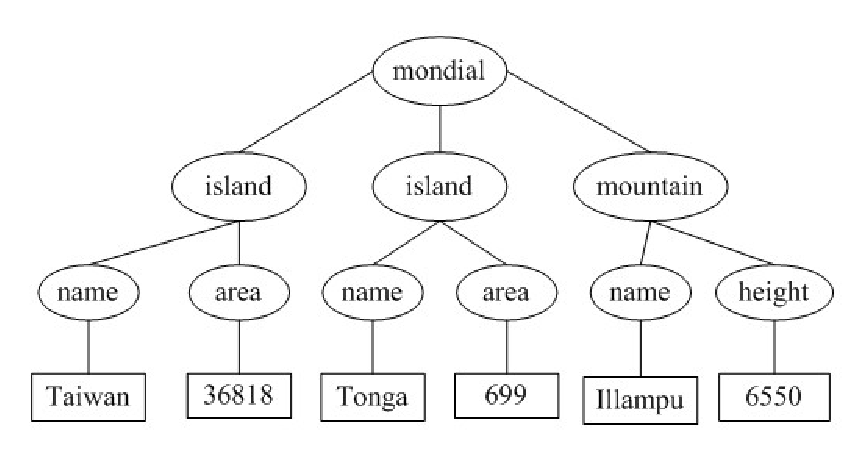
\includegraphics[width=0.4\textwidth]{XML}
\caption{树状结构}\label{fig:xml}
\vspace{\baselineskip}
\end{figure}


其插入图片的代码及其说明如下。
\vspace{1em}\noindent\hrule
\begin{verbatim}
\begin{figure}[H]
\centering
\includegraphics[width=0.4\textwidth]{文件名(.eps)}
\caption{标题}\label{标签名(通常为 fig:labelname)}
\vspace{\baselineskip} %表示图与正文空一行
\end{figure}
\end{verbatim}

\noindent\hrule

\begin{verbatim}
figure环境的可选参数[htbp]表示浮动图形所放置的位置,h (here)表示当前位置,t (top)表示页芯顶部,b (bottom)表示页芯底部,p (page)表示单独一页。在Word等软件中,图片通常插入到当前位置,如果当前页的剩余空间不够,图片将被移动到下一页,当前页就会出现很大的空白,其人工调整工作非常不便。由LaTeX提供的浮动图片功能,总是会按h->t->b->p的次序处理选项中的字母,自动调整图片的位置,大大减轻了工作量。
\centering命令将后续内容转换成每行皆居中的格式。
"\includegraphics"的可选参数用来设置图片插入文中的水平宽度,一般表示为正文宽度(\textwidth)的倍数。
\caption命令可选参数“标签名”为英文形式,一般不以图片或表格的数字顺序作为标签,而应包含一定的图片或表格信息,以便于文中引用(若图片、表格、公式、章节和参考文献等在文中出现的先后顺序发生了变化,其标注序号及其文中引用序号也会跟着发生变化,这一点是Word等软件所不能做到的)。另外,图题或表题并不会因为分页而与图片或表格体分置于两页,章节等各级标题也不会置于某页的最底部,LaTeX系统会自动调整它们在正文中的位置,这也是Word等软件所无法匹敌的。
\vspace将产生一定高度的竖直空白,必选参数为负值表示将后续文字位置向上提升,参数值可自行调整。em为长度单位,相当于大写字母M的宽度。\vspace{\baselineskip} 表示图与正文空一行。
引用方法:“见图~\ref{fig:figname}”、“如图~\ref{fig:figname}~所示”等。
\end{verbatim}

\noindent\hrule\vspace{1em}

若需要将~2~张及以上的图片并排插入到一行中,则需要采用\verb|minipage|环境,如图~\ref{fig:dd}~和图~\ref{fig:ds}~所示。
\begin{figure}[H]
\centering
\begin{minipage}{0.4\textwidth}
\centering
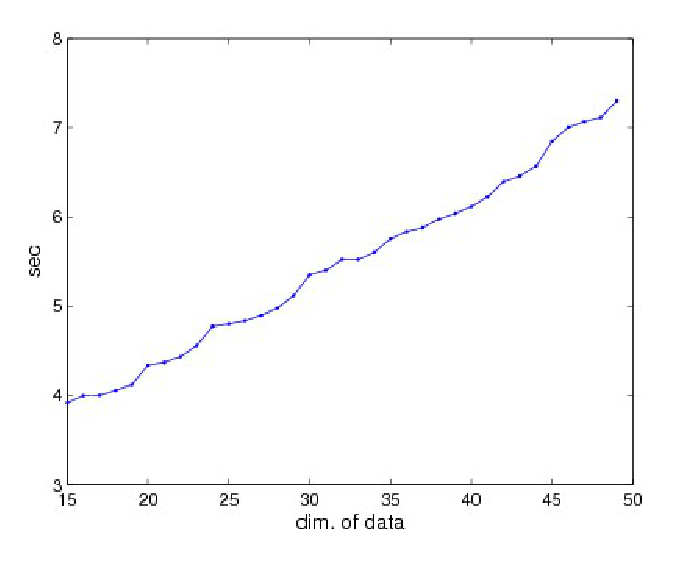
\includegraphics[width=\textwidth]{dataDimensions}
\caption{数据维数的变化}\label{fig:dd}
\end{minipage}
\begin{minipage}{0.4\textwidth}
\centering
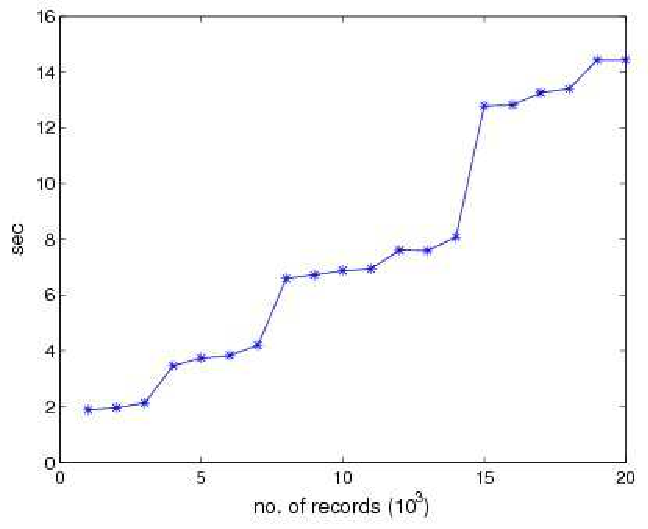
\includegraphics[width=\textwidth]{dataSize}
\caption{数据规模的变化}\label{fig:ds}
\end{minipage}
\vspace{\baselineskip}
\end{figure}

其代码如下所示。
\vspace{1em}\noindent\hrule
\begin{verbatim}
\begin{figure}[H]
\centering
\begin{minipage}{0.4\textwidth}
\centering
\includegraphics[width=\textwidth]{文件名}
\caption{标题}\label{fig:f1}
\end{minipage}
\begin{minipage}{0.4\textwidth}
\centering
\includegraphics[width=\textwidth]{文件名}
\caption{标题}\label{fig:f2}
\end{minipage}\vspace{\baselineskip}
\end{figure}
\end{verbatim}

\noindent\hrule

\begin{verbatim}
minipage环境的必选参数用来设置小页的宽度,若需要在一行中插入n个等宽图片,则每个小页的宽度应略小于(1/n)\textwidth。
\end{verbatim}

\noindent\hrule

\section{具有子图的图片插入方法}

图中若含有子图时,需要调用~subfigure~宏包, 如图~\ref{fig:subfig}~所示。
\begin{figure}[H]
  \centering
  \subfigure[Data Dimensions]{\label{fig:subfig:datadim}
                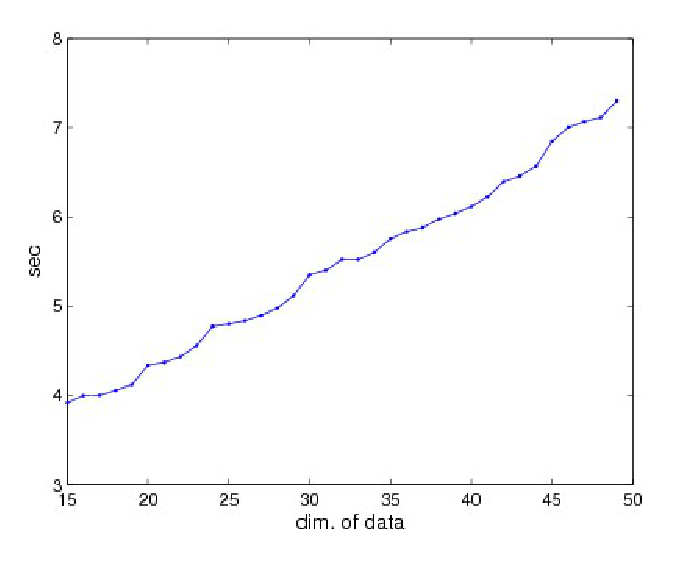
\includegraphics[width=0.4\textwidth]{dataDimensions}}
  \subfigure[Data Size]{\label{fig:subfig:datasize}
                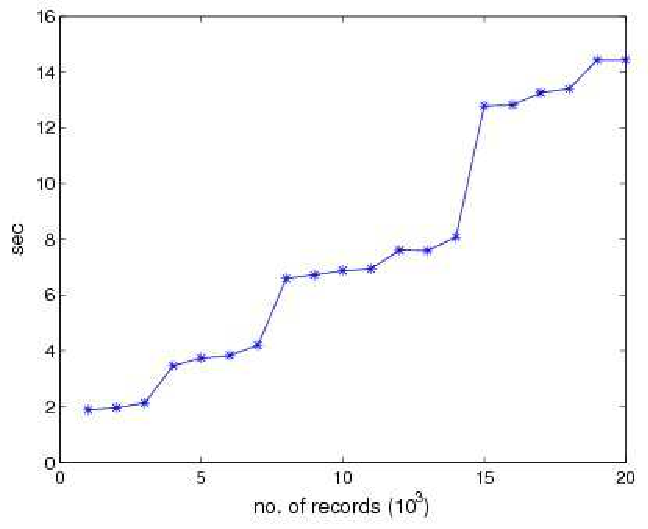
\includegraphics[width=0.4\textwidth]{dataSize}}
  \caption{Scalability of data}\label{fig:subfig}
\vspace{\baselineskip}
\end{figure}

其代码及其说明如下。
\vspace{1em}\noindent\hrule

\begin{verbatim}
\begin{figure}[H]
  \centering
  \subfigure[第1个子图标题]{
            \label{第1个子图标签(通常为 fig:subfig1:subsubfig1)}
            \includegraphics[width=0.4\textwidth]{文件名}}
  \subfigure[第2个子图标题]{
            \label{第2个子图标签(通常为 fig:subfig1:subsubfig2)}
            \includegraphics[width=0.4\textwidth]{文件名}}
  \caption{总标题}\label{总标签(通常为 fig:subfig1)}
\vspace{\baselineskip}
\end{figure}
\end{verbatim}

\noindent\hrule

\begin{verbatim}
子图的标签实际上可以随意设定,只要不重复就行。但为了更好的可读性,我们建议fig:subfig:subsubfig格式命名,这样我们从标签名就可以知道这是一个子图引用。
引用方法:总图的引用方法同本章第1节,子图的引用方法用\ref{fig:subfig:subsubfig}来代替。
\end{verbatim}

\noindent\hrule\vspace{1em}

子图的引用示例:如图~\ref{fig:subfig:datadim}~和图~\ref{fig:subfig:datasize}~所示。

若想获得插图方法的更多信息,参见网络上的~\href{ftp://ftp.tex.ac.uk/tex-archive/info/epslatex.pdf}{Using Imported Graphics in \LaTeX and pdf\LaTeX}~文档。 
%%% !Mode:: "TeX:UTF-8"

\chapter{表格的绘制方法}

\section{本科生毕业设计论文的绘表规范}

表应有自明性。表格不加左、右边线。表的编排建议采用国际通行的三线表。表内中文书写使用宋体五号字。

每个表格之上均应有表题(由表序和表名组成)。表序一般按章编排,如第~1~章第一个插表的序号为“表~1-1”等。表序与表名之间空两格,
表名使用中文五号字,居中。表名中不允许使用标点符号,表名后不加标点。
表头设计应简单明了,尽量不用斜线。表头中可采用化学,物理量等专业符号。

全表如用同一单位,则将单位符号移至表头右上角,加圆括号。
表中数据应准确无误,书写清楚。数字空缺的格内加横线“-”(占~2~个数字宽度)。表内文字或数字上、下或左、右相同时,
采用通栏处理方式,不允许用“〃”、“同上”之类的写法。

表内文字使用宋体五号字,垂直居中书写,起行空一格、转行顶格、句末不加标点。
如某个表需要转页接排,在随后的各页上应重复表的编号。编号后加“(续表)”,表题可省略。续表应重复表头。
表格绘制完成之后,与正文空一行。

\section{普通表格的绘制方法}

表格应具有三线表格式,因此需要调用~booktabs~宏包,其标准格式如表~\ref{tab:table1}~所示。
\begin{table}[htbp]
\caption{符合本科生毕业论文绘图规范的表格}\label{tab:table1}
\vspace{0.5em}\centering\wuhao
\begin{tabular}{ccccc}
\toprule[1.5pt]
$D$(in) & $P_u$(lbs) & $u_u$(in) & $\beta$ & $G_f$(psi.in)\\
\midrule[1pt]
 5 & 269.8 & 0.000674 & 1.79 & 0.04089\\
10 & 421.0 & 0.001035 & 3.59 & 0.04089\\
20 & 640.2 & 0.001565 & 7.18 & 0.04089\\
 5 & 269.8 & 0.000674 & 1.79 & 0.04089\\
10 & 421.0 & 0.001035 & 3.59 & 0.04089\\
20 & 640.2 & 0.001565 & 7.18 & 0.04089\\
 5 & 269.8 & 0.000674 & 1.79 & 0.04089\\
10 & 421.0 & 0.001035 & 3.59 & 0.04089\\
20 & 640.2 & 0.001565 & 7.18 & 0.04089\\
 5 & 269.8 & 0.000674 & 1.79 & 0.04089\\
10 & 421.0 & 0.001035 & 3.59 & 0.04089\\
20 & 640.2 & 0.001565 & 7.18 & 0.04089\\
\bottomrule[1.5pt]
\end{tabular}
\vspace{\baselineskip}
\end{table}

其绘制表格的代码及其说明如下。
\vspace{1em}\noindent\hrule

\begin{verbatim}
\begin{table}[htbp]
\caption{表标题}\label{标签名(通常为 tab:tablename)}
\vspace{0.5em}\centering\wuhao
\begin{tabular}{cc...c}
\toprule[1.5pt]
表头第1个格   & 表头第2个格   & ... & 表头第n个格  \\
\midrule[1pt]
表中数据(1,1) & 表中数据(1,2) & ... & 表中数据(1,n)\\
表中数据(2,1) & 表中数据(2,2) & ... & 表中数据(2,n)\\
表中数据(3,1) & 表中数据(3,2) & ... & 表中数据(3,n)\\
表中数据(4,1) & 表中数据(4,2) & ... & 表中数据(4,n)\\
...................................................\\
表中数据(m,1) & 表中数据(m,2) & ... & 表中数据(m,n)\\
\bottomrule[1.5pt]
\end{tabular}
\vspace{\baselineskip}
\end{table}
\end{verbatim}

\noindent\hrule

\begin{verbatim}
table环境是一个将表格嵌入文本的浮动环境。
\wuhao命令将表格的字号设置为五号字(10.5pt),在绘制表格结束退出时,不需要将字号再改回为\xiaosi,正文字号默认为小四号字(12pt)。
tabular环境的必选参数由每列对应一个格式字符所组成:c表示居中,l表示左对齐,r表示右对齐,其总个数应与表的列数相同。此外,@{文本}可以出现在任意两个上述的列格式之间,其中的文本将被插入每一行的同一位置。表格的各行以\\分隔,同一行的各列则以&分隔。
\toprule、\midrule和\bottomrule三个命令是由booktabs宏包提供的,其中\toprule和\bottomrule分别用来绘制表格的第一条(表格最顶部)和第三条(表格最底部)水平线,\midrule用来绘制第二条(表头之下)水平线,且第一条和第三条水平线的线宽为1.5pt,第二条水平线的线宽为1pt。
引用方法:“如表~\ref{tab:tablename}~所示”。
\end{verbatim}

\noindent\hrule

\section{长表格的绘制方法}

长表格是当表格在当前页排不下而需要转页接排的情况下所采用的一种表格环境。若长表格仍按照普通表格的绘制方法来获得,
其所使用的~\verb|table|~浮动环境无法实现表格的换页接排功能,表格下方过长部分会排在表格第~1~页的页脚以下。为了能够实现长表格的转页接排功能,
需要调用~\verb|longtable|~宏包,由于长表格是跨页的文本内容,因此只需要单独的~\verb|longtable|~环境,所绘制的长表格的格式如表~\ref{tab:table2}~所示。

此长表格~\ref{tab:table2}~第~2~页的标题“编号(续表)”和表头是通过代码自动添加上去的,无需人工添加,若表格在页面中的竖直位置发生了变化,长表格在第~2~页
及之后各页的标题和表头位置能够始终处于各页的最顶部,也无需人工调整,\LaTeX~系统的这一优点是~Word~等软件所无法企及的。

下段内容是为了让下面的长表格分居两页,看到表标题“编号(续表)”的效果。此模板的完成时间正值雨后初霁的四月二十五日,故引用林徽因《你是人间的四月天》全文:
\begin{center}
\begin{minipage}[c]{0.5\textwidth}

\textbf{你是人间的四月天}

\vspace{12pt}
我说你是人间的四月天\\
笑音点亮了四面风\\
轻灵在春的光艳中交舞着变\\
你是四月早天里的云烟\\
黄昏吹着风的软\\
星子在无意中闪\\
细雨点洒在花前\\
那轻~~那娉婷\\
你是鲜妍\\
百花的冠冕你戴着\\
你是天真~~庄严~~你是夜夜的月圆\\
雪化后那片鹅黄\\
你像~~新鲜初放芽的绿\\
你是柔嫩喜悦\\
水光浮动着你梦期待中白莲\\
你是一树一树的花开\\
是燕~~在梁间呢喃\\
你是爱~~是暖\\
是希望\\
你是人间的四月天
\end{minipage}
\end{center}

					
\wuhao\begin{longtable}{cc}
\caption{浙江工业大学各学院名称一览}\label{tab:table2}
 \vspace{0.5em}\\
\toprule[1.5pt] 学院名称 & 网址\\ \midrule[1pt]
\endfirsthead
\multicolumn{2}{c}{表~\thetable(续表)}\vspace{0.5em}\\
\toprule[1.5pt] 学院名称 & 网址\\ \midrule[1pt]
\endhead
\bottomrule[1.5pt]
\endfoot
法学院 & \url{http://www.law.zjut.edu.cn/}\\
化学工程与材料学院 &  \url{http://www.ce.zjut.edu.cn/}\\
机械工程学院 & \url{http://www.jdxy.zjut.edu.cn/}\\
信息工程学院 & \url{http://www.ie.zjut.edu.cn/}\\
计算机科学与技术学院 & \url{http://www.software.zjut.edu.cn/}\\
软件学院 & \url{http://www.software.zjut.edu.cn/}\\
经贸管理学院 & \url{http://www.cba.zjut.edu.cn/}\\
建筑工程学院& \url{http://www.jgxy.zjut.edu.cn/}\\
生物与环境工程学院 & \url{http://www.bee.zjut.edu.cn/}\\
理学院 & \url{http://www.lxy.zjut.edu.cn/}\\
教育科学与技术学院 & \url{http://www.et.zjut.edu.cn/}\\
人文学院 & \url{http://www.rwxy.zjut.edu.cn/}\\
健行学院 & \url{http://www.jxxy.zjut.edu.cn/}\\
外国语学院 & \url{http://www.fl.zjut.edu.cn/}\\
国际学院 & \url{http://www.gjxy.zjut.edu.cn/}\\
政治与公共管理学院 & \url{http://www.sppa.zjut.edu.cn/}\\
艺术学院 & \url{http://www.art.zjut.edu.cn/}\\
药学院 & \url{http://www.yxy.zjut.edu.cn/}\\
成人教育学院 & \url{http://www.cj.zjut.edu.cn/}\\
之江学院 & \url{http://www.zjc.zjut.edu.cn/}\\
研究生院 & \url{http://www.gs.zjut.edu.cn/}\\
\end{longtable}\xiaosi
\vspace{\baselineskip}

绘制长表格的代码及其说明如下。
\vspace{1em}\noindent\hrule

\begin{verbatim}
\wuhao\begin{longtable}{cc...c}
\caption{表标题}\label{标签名(通常为 tab:tablename)}\\
\toprule[1.5pt] 表头第1个格 & 表头第2个格 & ... & 表头第n个格\\ \midrule[1pt]
\endfirsthead
\multicolumn{n}{c}{表~\thetable(续表)}\vspace{0.5em}\\
\toprule[1.5pt] 表头第1个格 & 表头第2个格 & ... & 表头第n个格\\ \midrule[1pt]
\endhead
\bottomrule[1.5pt]
\endfoot
表中数据(1,1) & 表中数据(1,2) & ... & 表中数据(1,n)\\
表中数据(2,1) & 表中数据(2,2) & ... & 表中数据(2,n)\\
...................................................\\
表中数据(m,1) & 表中数据(m,2) & ... & 表中数据(m,n)\\
\end{longtable}\xiaosi
\end{verbatim}

\noindent\hrule
\begin{verbatim}
在绘制长表格的前面留出一个空白行,并在第2行的一开始全局定义长表格的字号为五号字,这样能够保证长表格之前段落的行距保持不变。
在绘制长表格结束后,需要\xiaosi命令重新将字号改为小四号字。
\endhead之前的文字描述的是第2页及其之后各页的标题或表头;
\endfirsthead之前的文字描述的是第1页的标题和表头,若无此命令,则第1页的表头和标题由\endhead命令确定;
同理,\endfoot之前的文字描述的是除最后一页之外每页的表格底部内容;
\endlastfoot之前的文字描述的是最后一页的表格底部内容,若无此命令,
则最后一页的表格底部内容由\endfoot命令确定;由于规范中长表格每页底部内容均相同(水平粗线),因此模板中没有用到\endlastfoot命令。
\end{verbatim}

\noindent\hrule
\section{列宽可调表格的绘制方法}
论文中能用到列宽可调表格的情况共有两种:一种是当插入的表格某一单元格内容过长以至于一行放不下的情况,
另一种是当对公式中首次出现的物理量符号进行注释的情况。这两种情况都需要调用~tabularx~宏包。下面将分别对这两种情况下可调表格的绘制方法进行阐述。
\subsection{表格内某单元格内容过长的情况}

首先给出这种情况下的一个例子如表~\ref{tab:table3}~所示。
\begin{table}[htbp]
\caption{最小的三个正整数的英文表示法}\label{tab:table3}
\vspace{0.5em}\wuhao
\begin{tabularx}{\textwidth}{llX}
\toprule[1.5pt]
Value & Name & Alternate names, and names for sets of the given size\\\midrule[1pt]
1 & One & ace, single, singleton, unary, unit, unity\\
2 & Two & binary, brace, couple, couplet, distich, deuce, double, doubleton, duad, duality, duet, duo, dyad, pair, snake eyes, span, twain, twosome, yoke\\
3 & Three & deuce-ace, leash, set, tercet, ternary, ternion, terzetto, threesome, tierce, trey, triad, trine, trinity, trio, triplet, troika, hat-trick\\\bottomrule[1.5pt]
\end{tabularx}
\vspace{\baselineskip}
\end{table}
绘制这种表格的代码及其说明如下。
\vspace{1em}\noindent\hrule
\begin{verbatim}
\begin{table}[htbp]
\caption{表标题}\label{标签名(通常为 tab:tablename)}
\vspace{0.5em}\wuhao
\begin{tabularx}{\textwidth}{l...X...l}
\toprule[1.5pt]
表头第1个格   & ... & 表头第X个格   & ... & 表头第n个格  \\
\midrule[1pt]
表中数据(1,1) & ... & 表中数据(1,X) & ... & 表中数据(1,n)\\
表中数据(2,1) & ... & 表中数据(2,X) & ... & 表中数据(2,n)\\
.........................................................\\
表中数据(m,1) & ... & 表中数据(m,X) & ... & 表中数据(m,n)\\
\bottomrule[1.5pt]
\end{tabularx}
\vspace{\baselineskip}
\end{table}
\end{verbatim}

\noindent\hrule
\begin{verbatim}
tabularx环境共有两个必选参数:第1个参数用来确定表格的总宽度,这里取为排版表格能达到的最大宽度——正文宽度\textwidth;第2个参数用来确定每列格式,其中标为X的项表示该列的宽度可调,其宽度值由表格总宽度确定。
标为X的列一般选为单元格内容过长而无法置于一行的列,这样使得该列内容能够根据表格总宽度自动分行。若列格式中存在不止一个X项,则这些标为X的列的列宽相同,因此,一般不将内容较短的列设为X。
标为X的列均为左对齐,因此其余列一般选为l(左对齐),这样可使得表格美观,但也可以选为c或r。
\end{verbatim}

\noindent\hrule
\subsection{对物理量符号进行注释的情况}
为使得对公式中物理量符号注释的转行与破折号“———”后第一个字对齐,此处最好采用表格环境。此表格无任何线条,左对齐,
且在破折号处对齐,一共有“式中”二字、物理量符号和注释三列,表格的总宽度可选为文本宽度,因此应该采用\verb|tabularx|环境。
由\verb|tabularx|环境生成的对公式中物理量符号进行注释的公式如式(\ref{eq:1})所示。
%\vspace*{10pt}

\begin{equation}\label{eq:1}
\ddot{\boldsymbol{\rho}}-\frac{\mu}{R_{t}^{3}}\left(3\mathbf{R_{t}}\frac{\mathbf{R_{t}\rho}}{R_{t}^{2}}-\boldsymbol{\rho}\right)=\mathbf{a}
\end{equation}

\begin{tabularx}{\textwidth}{@{}l@{\quad}r@{———}X@{}}
式中& $\bm{\rho}$ &追踪飞行器与目标飞行器之间的相对位置矢量;\\
&  $\bm{\ddot{\rho}}$&追踪飞行器与目标飞行器之间的相对加速度;\\
&  $\mathbf{a}$   &推力所产生的加速度;\\
&  $\mathbf{R_t}$ & 目标飞行器在惯性坐标系中的位置矢量;\\
&  $\omega_{t}$ & 目标飞行器的轨道角速度;\\
&  $\mathbf{g}$ & 重力加速度,$=\frac{\mu}{R_{t}^{3}}\left(
3\mathbf{R_{t}}\frac{\mathbf{R_{t}\rho}}{R_{t}^{2}}-\bm{\rho}\right)=\omega_{t}^{2}\frac{R_{t}}{p}\left(
3\mathbf{R_{t}}\frac{\mathbf{R_{t}\rho}}{R_{t}^{2}}-\bm{\rho}\right)$,这里~$p$~是目标飞行器的轨道半通径。
\end{tabularx}
\vspace{\wordsep}

其中生成注释部分的代码及其说明如下。

\vspace{1em}\noindent\hrule

\begin{verbatim}
\begin{tabularx}{\textwidth}{@{}l@{\quad}r@{— — —}X@{}}
式中 & symbol-1 & symbol-1的注释内容;\\
     & symbol-2 & symbol-2的注释内容;\\
     .............................;\\
     & symbol-m & symbol-m的注释内容。
\end{tabularx}\vspace{\wordsep}
\end{verbatim}

\noindent\hrule

\begin{verbatim}
   tabularx环境的第1个参数选为正文宽度,第2个参数里面各个符号的意义为:
   第1个@{}表示在“式中”二字左侧不插入任何文本,“式中”二字能够在正文中左对齐,若无此项,则“式中”二字左侧会留出一定的空白;
   @{\quad}表示在“式中”和物理量符号间插入一个空铅宽度的空白;
   @{— — —}实现插入破折号的功能,它由三个1/2的中文破折号构成;
   第2个@{}表示在注释内容靠近正文右边界的地方能够实现右对齐。
\end{verbatim}

\noindent\hrule\vspace{1em}

由此方法生成的注释内容应紧邻待注释公式并置于其下方,因此不能将代码放入~\verb|table|~浮动环境中。但此方法不能实现自动转页接排,
可能会在当前页剩余空间不够时,全部移动到下一页而导致当前页出现很大空白。因此在需要转页处理时,还请您手动将需要转页的代码放入一个
新的~\verb|tabularx|~环境中,将原来的一个~\verb|tabularx|~环境拆分为两个~\verb|tabularx|~环境。

若想获得绘制表格的更多信息,参见网络上的~\href{http://www.tug.org/pracjourn/2007-1/mori/}{Tables in \LaTeXe: Packages and Methods}~文档。


%%% !Mode:: "TeX:UTF-8"

\chapter{数学公式的输入方法}
\section{本科生毕业设计论文的公式规范}

论文中的公式应另起行,原则上应居中书写,与周围文字留有足够的空间区分开。
若公式前有文字(如“解”、“假定”等),文字空两格写,公式仍居中写。公式末不加标点。

公式应标注序号,并将序号置于括号内。 公式序号按章编排,如第~1~章第一个公式序号为“(1-1)”。公式的序号右端对齐。

公式较长时最好在等号“=”处转行,如难实现,则可在~$+$、$-$、$\times$、$\div$~运算符号处转行,转行时运算符号仅书写于转行式前,不重复书写。

文中引用公式时,一般用“见式~(1-1)”或“由公式~(1-1)”。

公式中用斜线表示“除”的关系时应采用括号,以免含糊不清,如~$a/(b\cos x)$。通常“乘”的关系在前,如~$a\cos x/b$而不写成~$(a/b)\cos x$。

不能用文字形式表示等式,如:$\textnormal{刚度}=\frac{{\textnormal{受力}}}{{\textnormal{受力方向的位移}}}$。

对于数学公式的输入方法,网络上有一个比较全面权威的文档\textbf{~\href{http://tug.ctan.org/cgi-bin/ctanPackageInformation.py?id=voss-mathmode}{Math mode}}~请大家事先大概浏览一下。下面将对学位论文中主要用到的数学公式排版形式进行阐述。

\section{生成~\LaTeX~数学公式的两种方法}
对于先前没有接触过~\LaTeX~的人来说,编写~\LaTeX~数学公式是一件很繁琐的事,尤其是对复杂的数学公式来说,更可以说是一件难以完成的任务。
实际上,生成~\LaTeX~数学公式有两种较为简便的方法,一种是基于~MathType~数学公式编辑器的方法,另一种是基于~MATLAB~商业数学软件的方法,
下面将分别对这两种数学公式的生成方法作一下简单介绍。

\subsection{基于~MathType~软件的数学公式生成方法}
MathType~是一款功能强大的数学公式编辑器软件,能够用来在文本环境中插入~Windows OLE~图形格式的复杂数学公式,所以应用比较普遍。但此软件只有~30~天的试用期,之后若再继续使用则需要付费购买才行。网络上有很多破解版的~MathType~软件可供下载免费使用,
笔者推荐下载安装版本号在~6.5~之上的中文破解版。

在安装好~MathType~之后,若在输入窗口中编写数学公式,复制到剪贴板上的仍然是图形格式的对象。
若希望得到可插入到~\LaTeX~编辑器中的文本格式对象,则需要对~MathType~软件做一下简单的设置:在~MathType~最上排的按钮中依次选择“参数选项
$\to$转换”,在弹出的对话窗中选中“转换到其它语言(文字):”,在转换下拉框中选择“Tex~--~--~LaTeX 2.09 and later”,并将对话框最下方的两个复选框全部勾掉,点击确定,这样,再从输入窗口中复制出来的对象就是文本格式的了,就可以直接将其粘贴到~\LaTeX~
编辑器中了。按照这种方法生成的数学公式两端分别有标记\verb|\[|和标记\verb|\]|,在这两个标记之间才是真正的数学公式代码。

若希望从~MathType~输入窗口中复制出来的对象为图形格式,则只需再选中“公示对象(Windows OLE~图形)”即可。

\subsection{基于~MATLAB~软件的数学公式生成方法}

MATLAB~是矩阵实验室(Matrix Laboratory)的简称,是美国~MathWorks~公司出品的商业数学软件。它是当今科研领域最常用的应用软件之一,
具有强大的矩阵计算、符号运算和数据可视化功能,是一种简单易用、可扩展的系统开发环境和平台。

MATLAB~中提供了一个~latex~函数,它可将符号表达式转化为~\LaTeX~数学公式的形式。其语法形式为~latex(s),其中,~s~为符号表达式,
之后再将~latex~函数的运算结果直接粘贴到~\LaTeX~编辑器中。从~\LaTeX~数学公式中可以发现,其中可能包含如下符号组合:

\begin{verbatim*}
\qquad=两个空铅(quad)宽度
\quad=一个空铅宽度
\;=5/18空铅宽度
\:=4/18空铅宽度
\,=3/18空铅宽度
\!=-3/18空铅宽度
\ =一个空格
\end{verbatim*}

所以最好将上述符号组合从数学公式中删除,从而使数学公式显得匀称美观。

对于~Word~等软件的使用者来说,在我们通过~MATLAB~运算得到符号表达式形式的运算结果时,在~Word~中插入运算结果需要借助于~MathType~软件,
通过在~MathType~中输入和~MATLAB~运算结果相对应的数学表达形式,之后再将~MathType~数学表达式转换为图形格式粘贴到~Word~中。实际上,
也可以将~MATLAB~中采用~latex~函数运行的结果直接粘贴到~MathType~中,再继续上述步骤,这样可以大大节省输入公式所需要的时间。
此方法在~MathType~6.5c~上验证通过,若您粘入到~MathType~中的仍然为从~MATLAB~中导入的代码,请您更新~MathType~软件。

\section{数学字体}
在数学模式下,常用的数学字体命令有如下几种:

\begin{verbatim}
\mathnormal或无命令 用数学字体打印文本;
\mathit             用斜体(\itshape)打印文本;
\mathbf             用粗体(\bfseries)打印文本;
\mathrm             用罗马体(\rmfamily)打印文本;
\mathsf             用无衬线字体(\sffamily)打印文本;
\mathtt             用打印机字体(\ttfamily)打印文本;
\mathcal            用书写体打印文本;
\end{verbatim}

在学位论文撰写中,只需要用到上面提到的~\verb|\mathit|、\verb|\mathbf|~和~\verb|\mathrm|~命令。若要得到~Times New Roman~的数学字体,则需要调用~txfonts~宏包(此宏包实际上采用的是~Nimbus Roman No9 L~字体,
它是开源系统中使用的免费字体,其字符字体与~Times New Roman~字体几乎完全相同);若要得到粗体数学字体,则需要调用~bm~宏包。表~\ref{tab:fonts}~中分别列出了得到阿拉伯数字、拉丁字母和希腊字母
各种数学字体的命令。

\begin{table}[htbp]
\caption{常用数学字体命令一览}\label{tab:fonts}
\vspace{0.5em}\centering\wuhao
\begin{tabular}{llll}
\toprule
 & 阿拉伯数字\&大写希腊字母 & 大小写拉丁字母 & 小写希腊字母  \\
\midrule
斜体 & \verb|\mathit{}| & \verb|无命令| & \verb|无命令|\\
粗斜体 & \verb|\bm{\mathit{}}| & \verb|\bm{}| & \verb|\bm{}|\\
直立体 & \verb|无命令| & \verb|\mathrm{}| & \verb|字母后加up|\\
粗体 & \verb|\mathbf{}或\bm{}| & \verb|\mathbf{}| & \verb|\bm{字母后加up}|\\
\bottomrule
\end{tabular}
\vspace{\baselineskip}
\end{table}

\noindent 下面列出了一些应采用直立数学字体的数学常数和数学符号。

\section{行内公式}
出现在正文一行之内的公式称为行内公式,例如~$f(x)=\int_{a}^{b}\frac{\sin{x}}{x}dx$。对于非矩阵和非多行形式的行内公式,一般不会使得行距发生变化,而~Word~等软件却会根据行内公式的竖直距离而自动调节行距,如图~\ref{fig:hangju}~所示。

\begin{figure}[htbp]
\centering
\subfigure[由~\LaTeX~系统生成的行内公式]{\label{fig:subfig:latex}
                \fbox{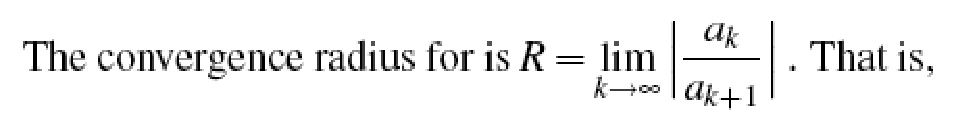
\includegraphics[width=0.55\textwidth]{latex}}}
\subfigure[由~Word软件生成的~.doc~格式行内公式]{\label{fig:subfig:word}
                \fbox{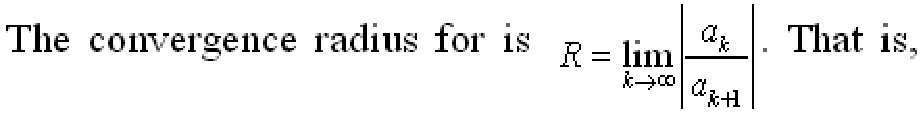
\includegraphics[width=0.55\textwidth]{word}}}
\subfigure[由~Word软件生成的~.pdf~格式行内公式]{\label{fig:subfig:pdf}
                \fbox{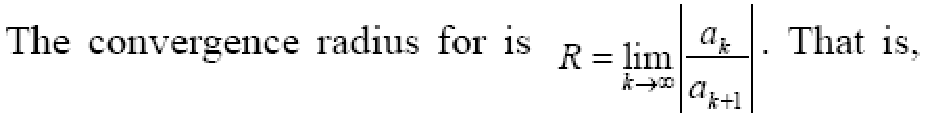
\includegraphics[width=0.55\textwidth]{pdf}}}

\caption{由~\LaTeX~和~Word~生成的~3~种行内公式屏显效果}\label{fig:hangju}
\vspace{-1em}
\end{figure}

这三幅图分别为~\LaTeX~和~Word~生成的行内公式屏显效果,从图中可看出,在~\LaTeX~文本含有公式的行内,在正文与公式之间对接工整,行距不变;而在~Word~文本含有公式的行内,在正文与公式之间对接不齐,行距变大。因此从这一点来说,
\LaTeX~系统在数学公式的排版上具有很大优势。

\LaTeX~提供的行内公式最简单、最有效的方法是采用~\TeX~本来的标记———开始和结束标记都写作~\$,例如本段开始的例子可由下面的输入得到。
\verb|$f(x)=\int_{a}^{b}\frac{\sin{x}}{x}\mathrm{d}x$|

\section{行间公式}
位于两行之间的公式称为行间公式,每个公式都是一个单独的段落,例如
\[\int_a^b{f\left(x\right)dx}=\lim_{\left\|\Delta{x_i}\right\|\to 0}\sum_i{f\left(\xi_i\right)\Delta{x_i}}\]
除人工编号外,\LaTeX~各种类型行间公式的标记见表~\ref{tab:eqtag}。
\begin{table}[htbp]
\caption{各种类型行间公式的标记}\label{tab:eqtag}
\vspace{0.5em}\centering\wuhao
\begin{tabularx}{\textwidth}{cll}
\toprule
& 无编号 & 自动编号\\
\midrule
单行公式& \verb|\begin{displaymath}... \end{displaymath}|& \verb|\begin{equation}... \end{equation}|\\
        & 或~\verb|\[...\]| & \\
多行公式& \verb|\begin{eqnarray*}... \end{eqnarray*}|& \verb|\begin{eqnarray}... \end{eqnarray}|\\
\bottomrule
\end{tabularx}
\end{table}

另外,在自动编号的某行公式行尾添加标签~\verb|\nonumber|,可将该行转换为无编号形式。

行间多行公式需采用~\verb|eqnarray|~或~\verb|eqnarray*|~环境,它默认是一个列格式为~\verb|rcl|~的~3~列矩阵,并且中间列的字号要小一些,因此通常只将需要对齐的运算符号(通常为等号“=”)置于中间列。

\section{可自动调整大小的定界符}
若在左右两个定界符之前分别添加命令~\verb|\left|~和~\verb|\right|,则定界符可根据所包围公式大小自动调整其尺寸,这可从式(\ref{nodelimiter})和式(\ref{delimiter})中看出。
\begin{equation}\label{nodelimiter}
(\sum_{k=\frac12}^{N^2})
\end{equation}
\begin{equation}\label{delimiter}
\left(\sum_{k=\frac12}^{N^2}\right)
\end{equation}
式(\ref{nodelimiter})和式(\ref{delimiter})是在~\LaTeX~中分别输入如下代码得到的。
\begin{verbatim}
(\sum_{k=\frac12}^{N^2})
\left(\sum_{k=\frac12}^{N^2}\right)
\end{verbatim}
\verb|\left|~和~\verb|\right|~总是成对出现的,若只需在公式一侧有可自动调整大小的定界符,则只要用“.”代替另一侧那个无需打印出来的定界符即可。

若想获得关于此部分内容的更多信息,可参见~\href{http://tug.ctan.org/cgi-bin/ctanPackageInformation.py?id=voss-mathmode}{Math mode}~文档的第~8~章“Brackets, braces and parentheses”。

\section{数学重音符号}
数学重音符号通常用来区分同一字母表示的不同变量,输入方法如下(需要调用~\verb|amsmath|~宏包):

\vspace{0.5em}{\noindent\wuhao\begin{tabularx}{\textwidth}{Xc|Xc|Xc}
 \verb|\acute| & $\acute{a}$ & \verb|\mathring| & $\mathring{a}$ & \verb|\underbrace| & $\underbrace{a}$ \\
 \verb|\bar| & $\bar{a}$ & \verb|\overbrace| & $\overbrace{a}$ & \verb|\underleftarrow| & $\underleftarrow{a}$ \\
 \verb|\breve| & $\breve{a}$ & \verb|\overleftarrow| & $\overleftarrow{a}$ & \verb|\underleftrightarrow| & $\underleftrightarrow{a}$ \\
 \verb|\check| & $\check{a}$ & \verb|\overleftrightarrow| & $\overleftrightarrow{a}$ & \verb|\underline| & $\underline{a}$ \\
 \verb|\dddot| & $\dddot{a}$ & \verb|\overline| & $\overline{a}$ & \verb|\underrightarrow| & $\underrightarrow{a}$ \\
 \verb|\ddot| & $\ddot{a}$ & \verb|\overrightarrow| & $\overrightarrow{a}$ & \verb|\vec| & $\vec{a}$ \\
 \verb|\dot| & $\dot{a}$ & \verb|\tilde| & $\tilde{a}$ & \verb|\widehat| & $\widehat{a}$ \\
 \verb|\grave| & $\grave{a}$ & \verb|\underbar| & $\underbar{a}$ & \verb|\widetilde| & $\widetilde{a}$ \\
 \verb|\hat| & $\hat{a}$
\end{tabularx}}\vspace{0.5em}
当需要在字母~$i$~和~$j$~的上方添加重音符号时,为了去掉这两个字母顶上的小点,这两个字母应该分别改用~\verb|\imath|~和~\verb|\jmath|。

如果遇到某些符号不知道该采用什么命令能输出它时,则可通过~\href{http://detexify.kirelabs.org/classify.html}{Detexify$^2$~网站}来获取符号命令。若用鼠标左键在此网页的方框区域内画出你所要找的符号形状,则会在网页右方列出和你所画符号形状相近的~5~个符号及其相对应的~\LaTeX~输入命令。若所列出的符号中不包括你所要找的符号,还可通过点击“Select from the complete list!”的链接以得分从低到高的顺序列出所有符号及其相对应的~\LaTeX~输入命令。

最后,建议大家还以~\href{http://tug.ctan.org/cgi-bin/ctanPackageInformation.py?id=voss-mathmode}{Math mode}~这篇~pdf~文档作为主要参考。若要获得最为标准、美观的数学公式排版形式,可以查查文档中是否有和你所要的排版形式相同或相近的代码段,通过修改代码段以获得你所要的数学公式排版形式。


%%% !Mode:: "TeX:UTF-8"

\chapter{罗列、定理和代码环境使用方法}

\section{单层罗列环境}

浙江工业大学毕业设计论文一般可采用两种罗列环境:一种是并列条目有同样标签的~\verb|itemize|~罗列环境,另一种是具有自动排序编号符号的~\verb|enumerate|~罗列环境。这两种罗列环境的样式参数可参考图~\ref{fig:list}。
\begin{figure}[htbp]
\centering
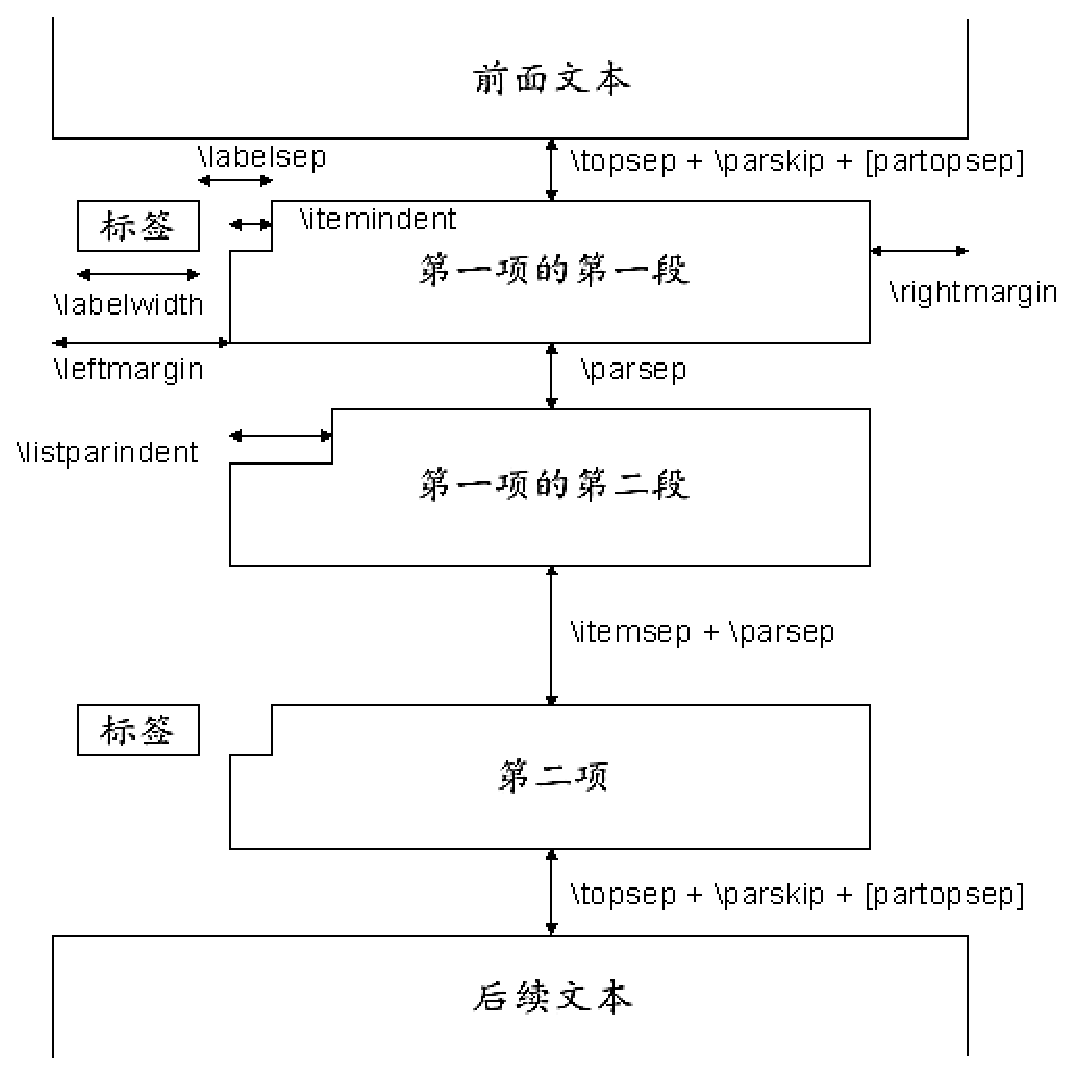
\includegraphics[width = 0.6\textwidth]{list}
\caption{罗列环境参数示意图}\label{fig:list}\vspace{-1em}
\end{figure}

通过调用~enumitem~宏包可以很方便地控制罗列环境的布局,其~format.tex~文件中的~\verb|\setitemize|~和~\verb|\setenumerate|~命令分别用来设置~\verb|itemize|~和~\verb|enumerate|~环境的样式参数。采用~\verb|itemize|~单层罗列环境的排版形式如下:

\begin{itemize}
\item 第一个条目文本内容
\item 第二个条目文本内容
\item 第三个条目文本内容
\end{itemize}

其代码如下

\begin{verbatim}
\begin{itemize}
  \item 第一个条目文本内容
  \item 第二个条目文本内容
  ...
  \item 第三个条目文本内容
\end{itemize}
\end{verbatim}

采用~\verb|enumerate|~单层罗列环境的排版形式如下:

\begin{enumerate}
\item 第一个条目文本内容
\item 第二个条目文本内容
\item 第三个条目文本内容
\end{enumerate}

其代码如下

\begin{verbatim}
\begin{enumerate}
  \item 第一个条目文本内容
  \item 第二个条目文本内容
  ...
  \item 第三个条目文本内容
\end{enumerate}
\end{verbatim}



\section{定理环境}

\begin{definition}[谱半径]\label{def:def1}
  称~$n$~阶方阵~$\mathbf{A}$~的全体特征值~$\lambda_1,\cdots,\lambda_n$~组成的集合为~$\mathbf{A}$~的谱,称
  $$\rho(\mathbf{A})=\max{\{|\lambda_1|,\cdots,|\lambda_n|\}}$$
\end{definition}
\begin{theorem}[相似充要条件]\label{lemma:l1}
  方阵$A$和$B$相似的充要条件是:~$A$~和~$B$~有全同的不变因子。
\end{theorem}
\begin{corollary}[推论1]\label{cor:cor1}
在赋范空间~$(X,\|\cdot\|)$~上定义~$d(x,y)=\|x-y\|$, 对任意~$x,y\in X$,~则~$(X,d)$~是距离空间。
\end{corollary}
\begin{proof}
  只需证明~$d(x,y)$~是距离。
\end{proof}
\newpage

定义代码如下:
\begin{verbatim}
 \begin{definition}[谱半径]\label{def:def1}
  称~$n$~阶方阵~$\mathbf{A}$~的全体特征值
  $\lambda_1,\cdots,\lambda_n$组成的集合为~$\mathbf{A}$~的谱,称
  $$\rho(\mathbf{A})=\max{\{|\lambda_1|,\cdots,|\lambda_n|\}}$$
\end{definition}
\end{verbatim}
\noindent\hrule

\vspace{0.1em}\noindent\hrule
\vspace{1em}
定理代码如下:
\begin{verbatim}
\begin{theorem}[相似充要条件]\label{lemma:l1}
  方阵$A$和$B$相似的充要条件是:$A$和$B$有全同的不变因子。
\end{theorem}
\end{verbatim}

\noindent\hrule\vspace{0.1em}

\noindent\hrule
\vspace{1em}
推论和证明代码如下:
\begin{verbatim}
\begin{corollary}[推论1]\label{cor:cor1}
在赋范空间~$(X,\|\cdot\|)$~上定义$d(x,y)=\|x-y\|$,
对任意$x,y\in X$,则$(X,d)$是距离空间。
\end{corollary}
\begin{proof}
  只需证明$d(x,y)$是距离。
\end{proof}
\end{verbatim}
\noindent\hrule\vspace{1em}

定理定义[]中是可选参数,用来说明定理的名称。其他环境格式书写与上面定理、定义、推论格式相同,可自己调用其他环境。
若需要书写定理定义等内容,而且带有顺序编号,需要采用如下环境。除了~\verb|proof|~环境之外,其余~9~个环境都可以有一个可选参数作为附加标题。

\begin{center}
\vspace{0.5em}\noindent\wuhao\begin{tabularx}{0.7\textwidth}{lX|lX}
定理 & \verb|theorem|~环境 & 定义 & \verb|definition|~环境 \\
例 & \verb|example|~环境 & 算法 & \verb|algorithm|~环境 \\
公理 & \verb|axiom|~环境 & 命题 & \verb|proposition|~环境 \\
引理 & \verb|lemma|~环境 & 推论 & \verb|corollary|~环境 \\
注解 & \verb|remark|~环境 & 证明 & \verb|proof|~环境 \\
\end{tabularx}
\end{center}
\section{代码环境}
很多和计算机专业背景相关的同学都会使用到代码环境,使用~\verb|\verb|~指令或者是~\verb|verbatim|~环境固然是一种选择,但是比不上专门的~lstlisting~环境这么专业。
\begin{lstlisting}[language=C]
int main(int argc, char ** argv)
{
	printf("Hello world!\n");
	return 0;
}
\end{lstlisting}

\noindent\hrule
\vspace{0.1em}\noindent\hrule

\vspace{1em}

\noindent 代码如下:
\begin{verbatim}
\begin{lstlisting}[language=C]
int main(int argc, char ** argv)
{
	printf("Hello world!\n");
	return 0;
}
\end{lstlisting}
\end{verbatim}
\noindent\hrule\vspace{1em}

在代码中显示的关键字为蓝色,框的左侧显示的是行号,这样便于读者阅读和查找代码,同时添加了浅蓝色的阴影边框,达到了美观的效果。
代码环境的设置已在~package~中~\verb|\lstset|~指令中定义。定义中支持跨页显示,可以将较长的代码置于~lstlisting~环境中。
\section{算法环境}
很多和计算机专业背景相关的同学会使用到算法环境,之前使用到的定理环境固然是一种选择,但是比不上专门的~algorithm2e~环境这么专业。为了实现专业和接近完美,本版本支持算法环境。如下所示:
\begin{algorithm}[htbp]
    \caption{算法标题}
    \label{alg:demoAlgo} % 贴上标签以便交叉引用
    \begin{algorithmic}[1]  % 这个 1 表示每一行都显示数字
    \STATE 初始化...
    \FOR{$i=0;i\le M; i\rightarrow i + 1$}
        \STATE 执行语句~1;
        \STATE 执行语句~2;
        \STATE ...
    \ENDFOR
    \STATE ...
    \WHILE{某条件}
        \STATE 执行语句~1;
        \STATE 执行语句~2;
        \STATE ...
    \ENDWHILE
    \STATE ...
    \end{algorithmic}
\end{algorithm}
\noindent\hrule
\vspace{0.1em}\noindent\hrule

\vspace{1em}

\noindent 代码如下:
\begin{verbatim}
  \begin{algorithm}[htbp]
    \caption{算法标题}
    \label{alg:demoAlgo} % 贴上标签以便交叉引用
    \begin{algorithmic}[1]  % 这个 1 表示每一行都显示数字
    \STATE 初始化...
    \FOR{$i=0;i\le M; i\rightarrow i + 1$}
        \STATE 执行语句~1;
        \STATE 执行语句~2;
        \STATE ...
    \ENDFOR
    \STATE ...
    \WHILE{某条件}
        \STATE 执行语句~1;
        \STATE 执行语句~2;
        \STATE ...
    \ENDWHILE
    \STATE ...
    \end{algorithmic}
\end{algorithm}
\end{verbatim}


%%% !Mode:: "TeX:UTF-8"

\chapter{总结与展望}
随着我国高等教育规模的不断扩大,教学质量的不断提高,研究项目的不断增多,信息化程不断增高,基于互联网的项目申报系统将日益受到重视[27]。传统的纸质项目申报评审方式面临着很大的挑战,迫切要求我们实现项目申报评审的科学化、现代化。对此,网上项目申报评审系统的开发日益迫切,项目的开发意义也越来越重要。

	“浙江省教育厅教育质量与教学改革项目申报管理系统”是一个集项目信息发布、项目管理、项目网上申报评审管和项目成果展示为一体的信息化管理系统。为用户提供一个方便、快捷、透明、高效的项目申报评审环境。系统的实现将有效的提高项目主管部门、学校、老师的工作效率,带来巨大的经济效益。

\end{verbatim}
那么,编译的时候就只编译未加~\%~的一章,在这个例子中,即本章~intros。

理论上,并不一定要把每章放在不同的文件中。但是这种自顶向下,分章节写作、编译的方法有利于提高效率,大大减少~Debug~过程中的编译时间,同时减小风险。

\section{参考文献生成方法}

\LaTeX~具有插入参考文献的能力。Google Scholar~网站上存在兼容~BibTeX~的参考文献信息,通过以下几个步骤,可以轻松完成参考文献的生成。
\begin{itemize}
  \item 在\href{http://scholar.google.com/}{谷歌学术搜索}中,
        点击\href{http://scholar.google.com/scholar_preferences?hl=en&as_sdt=0,5}{学术搜索设置}。
  \item 页面打开之后,在\textbf{文献管理软件}选项中选择\textbf{显示导入~BibTeX~的链接},单击保存设置,退出。
  \item 在谷歌学术搜索中检索到文献后,在文献条目区域单击导入~BibTeX~选项,页面中出现文献的引用信息。
  \item 将文献引用信息的内容复制之后,添加到~references~文件夹下的~reference.bib~中。
\end{itemize}

\section{编译注意事项}
\begin{enumerate}
  \item 由于模板使用~UTF-8~编码,所以源文件应该保存成~UTF-8~格式,否则可能出现中文字符无法识别的错误。
  本模板中每一个~.tex~文件的文件的开头已经加上一行:\\
  \verb|% !Mode:: "TeX:UTF-8"|\\
     这样可以确保~.tex~文件默认使用~UTF-8~的格式打开。读者如果删去此行,很有可能会导致中文字符显示乱码。
     在~WinEdt~编辑器中可以使用以下两种方式保存成~UTF-8~格式:
      \begin{enumerate}
        \item 先建立~.tex~文件,另存为~.tex~文件时,选择用~UTF-8~格式保存。
        \item
            在~WinEdt~编辑器中,选择\\
            \mbox{~Document$\to$Document Settings$\to$Document Mode $\to$TeX:UTF-8} 同时在\\~WinEdt~最下面的状态栏中,可以看到该文档是~TeX~格式还是~TeX:UTF-8~格式。
            当文档为~TeX:UTF-8~格式时,状态栏一般显示:\\
            \makebox[\textwidth][l]{Wrap | Indent | INS | LINE |Spell | TeX:UTF-8 | -src~等。}
      \end{enumerate}
  \item 如果在pdf书签中,中文显示乱码的话,则注意以下说明:
    \begin{verbatim}
        \usepackage{CJKutf8}
        % 1. 如果使用CJKutf8
        %    Hyperref中应使用unicode参数
        % 2. 如果使用CJK
        %    Hyperref则使用CJKbookmarks参数
        %    可惜得到的PDF书签是乱码,建议弃用
        % 3. Unicode选项和CJKbookmarks不能同时使用
        \usepackage[
        %CJKbookmarks=true,
        unicode=true
        ]{hyperref}
     \end{verbatim}
  \item 建议采用以下两种编译方式:
  \begin{enumerate}
    \item xelatex + bibtex + xelatex + xelatex, 在这种编译情况下,所有图片文件应该保存成~.eps~格式,如~figures~文件夹里~.eps~图片。
  \end{enumerate}
\end{enumerate}

\section{系统要求}
    CTEX 2.8, MiKTeX 2.8 或者 TeX Live 2009。使用推荐的~WinEdt 6.0~编辑器,可以完成文件的编辑和编译工作。

\section{\TeX~简介}

以下内容是~milksea@bbs.ctex.org~撰写的关于~\TeX~的简单介绍,略有改动。
注意这不是一个入门教程,不讲~\TeX~系统的配置安装,也不讲具体的~\XeLaTeX~代码。
这里仅仅试图以一些只言片语来解释:
进入这个门槛之前新手应该知道的注意事项,以及遇到问题以后该去如何解决问题。

\subsection{什么是 \TeX/\XeLaTeX,我是否应该选择它~?}

\TeX~是最早由高德纳(Donald Knuth)教授创建的一门标记式宏语言,
用来排版科技文章,尤其擅长处理复杂的数学公式。\TeX~同时也是处理这一语言的排版软件。
\XeLaTeX~是 Leslie Lamport 在~\TeX~基础上按内容/格式分离和模块化等思想建立的一集~\TeX~上的格式。

\TeX~本身的领域是专业排版领域
但现在~TeX/LaTeX~也被广泛用于生成电子文档甚至幻灯片等,~\TeX~语言的数学部分
偶尔也在其他一些地方使用。但注意~\TeX~并不适用于文书处理(Microsoft Office 的领域,以前和现在都不是)。

选择使用~\TeX/\XeLaTeX~的理由包括:
\begin{itemize}
\item 免费软件;
\item 专业的排版效果;
\item 是事实上的专业数学排版标准;
\item 广泛的西文期刊接收甚或只接收 LaTeX 格式的投稿;
\item[] ……
\end{itemize}
不选择使用~\TeX/\XeLaTeX~的理由包括:
\begin{itemize}
\item 需要相当精力学习;
\item 图文混合排版能力不够强;
\item 仅在数学、物理、计算机等领域流行;
\item 中文期刊的支持较差;
\item[] ……
\end{itemize}

请尽量清醒看待网上经常见到的关于~\TeX~与其他软件的优劣比较和口水战。在选择使用或离开之前,请先考虑
\TeX~的应用领域,想想它是否适合你的需要。


\subsection{我该用什么编辑器~?}

编辑器功能有简有繁,特色不一,从简单的纯文本编辑器到繁复的 Emacs,因人而易。基本功能有语法高亮、方便编译预览就很好了,扩充功能和定制有无限的可能。初学者可以使用功能简单、使用方便的专用编辑器,如 ~TeXWorks、Kile、WinEdt~等,或者类似所见即所得功能的~LyX;熟悉的人可以使用定制性更强的~Notepad++、SciTE、Vim、Emacs ~等。这方面的介绍很多,一开始不妨多试几种,找到最适合自己的才是最好的。

另外提醒一句,编辑器只是工作的助手,不必把它看得太重。

\subsection{我应该看什么~\XeLaTeX~读物~?}

这不是一个容易回答的问题,因为有许多选择,也同样有许多不合适的选择。
这里只是选出一个比较好的答案。更多更详细的介绍可以在版面和网上寻找(注意时效)。

近两年~\TeX~的中文处理发展很快,目前没有哪本书在中文处理方面给出一个最新进展的合适综述,
因而下面的介绍也不主要考虑中文处理。

\begin{enumerate}

\item 我能阅读英文。
\begin{enumerate}
\item 迅速入门:ltxprimer.pdf (LaTeX Tutorials: A Primer, India TUG)
\item 系统学习:A Guide to LaTeX, 4th Edition, Addison-Wesley
               有机械工业出版社的影印版(《\LaTeX{}~实用教程》)
\item 深入学习:要读许多书和文档,TeXbook 是必读的
\item 细节学习:去读你使用的每一个宏包的说明文档
\item 专题学习:阅读讲数学公式、图形、表格、字体等的专题文档
\end{enumerate}

\item 我更愿意阅读中文。
\begin{enumerate}
\item 迅速入门:lnotes.pdf (LaTeX Notes, 1.20, Alpha Huang)
\item 系统学习:《\LaTeXe{}~科技排版指南》,邓建松(电子版)
      如果不好找,可以阅读《\LaTeXe~入门与提高》第二版,陈志杰等,或者 《\LaTeXe~完全学习手册》,胡伟
\item 深入学习:~TeXbook0.pdf~(特可爱原本,TeXbook 的中译,xianxian)
\item 具体问题释疑:~CTeX-FAQ.pdf~,\\
        吴凌云,~\url{http://www.ctex.org/CTeXFAQ}~
\end{enumerate}
\end{enumerate}

遇见问题和解决问题的过程可以快速提高自己的技能,建议此时:
\begin{itemize}
  \item 利用~Google~搜索。
  \item 清楚,扼要地提出你的问题。
\end{itemize}

\subsection{什么知识会过时~?什么不会~?}

\TeX~是排版语言,也是广泛使用的软件,并且不断在发展中;
因此,总有一些东西会很快过时。作为学习~\TeX~的人,
免不了要看各种各样的书籍、电子文档和网络论坛上的只言片语,
因此了解什么知识会迅速过时,什么知识不会是十分重要的。

最稳定的是关于~Primitive \TeX~和~Plain \TeX~的知识,也就是 Knuth
在他的《The TeXbook》中介绍的内容。因为~\TeX~
系统开发的初衷就是稳定性,要求今天的文档到很久以后仍可以得到完全相同的结果,
因此 Knuth 限定了他的~\TeX~语言和相关实现的命令、语法。这些内容许多年来就没有多少变化,
在未来的一些年里也不会有什么变化。
Primitive \TeX~和 Plain \TeX~的知识主要包括 \TeX~排版的基本算法和原理,
盒子的原理,底层的 \TeX~命令等。其中技巧性的东西大多在宏包设计中,
初学者一般不会接触到很多;而基本原理则是常常被提到的,
譬如,~\TeX~把一切排版内容作为盒子(box)处理。

相对稳定的是关于基本~\LaTeXe~
的知识,也包括围绕~\LaTeXe~的一些核心宏包的知识。
在可预见的将来,~\LaTeXe~不会过时。
\LaTeXe~的知识是目前大部分~\LaTeX~书籍的主体内容。关于~\XeLaTeX~的标准文档类
~(article、report、book、letter、slide~等),关于基本数学公式的输入,
文档的章节层次,表格和矩阵,图表浮动体,LR 盒子与段落盒子……
这些~\XeLaTeX~的核心内容都是最常用的,相对稳定的。
与~\LaTeXe~相匹配的核心宏包,
如~graphics(x)、ifthen、fontenc、doc~等,也同样是相对稳定的。
还有一些被非常广泛应用的宏包,如~amsmath~系列,也可以看作是相对稳定的。

简单地说,关于基本~\TeX/\XeLaTeX~的语言,都是比较稳定的。与之对应,实现或者支持~\TeX/\XeLaTeX~语言的软件,
包括在~\TeX/\XeLaTeX~基础上建立的新的宏,都不大稳定。

容易过时的是关于第三方~\XeLaTeX~宏包的知识、第三方~\TeX~工具的知识,以及新兴~\TeX~相关软件的知识等。
~\TeX~和~\XeLaTeX~语言是追求稳定的;但无论是宏包还是工具,作为不断更新软件,它们是不稳定的。
容易过时的技术很多,而且现在广泛地出现在几乎所有~\XeLaTeX~文档之中,因此需要特别引起注意:
宏包的过时的原因可能是宏包本身的升级换代带来了新功能或不兼容,
也可能是同一功能的更新更好的宏包代替了旧的宏包。前者的典型例子比如绘图宏包~PGF/TikZ~,
现在的~2.00~版功能十分强大,和旧的~1.1x~版相差很大,和更旧的~0.x~版本则几乎完全不同;后
者的典型例子比如~caption~宏包先是被更新的~caption2~宏包代替,后来~caption~宏包更新又使得
caption2 宏包完全过时。——安装更新的发行版可以避免使用过旧的宏包;
认真阅读宏包自带的文档而不是搜索得到的陈旧片断可以避免采用过时的代码。

工具过时的主要原因也是升级换代和被其他工具替换。前者的典型例子是编辑器
WinEdt~在~5.5~以后的版本支持~UTF-8~编码,而旧版本不支持;
后者的典型例子是中文字体安装工具从~GBKFonts~到~xGBKFonts~到~FontsGen~不断被取代。
图形插入是一个在~\TeX~实现、宏包与外围工具方面都更新很快的东西。
在过去,最常用的输出格式是~PS(PostScript)~格式,因此插入的图像以~EPS~为主流。
使用~Dvips~为主要输出工具,外围工具有~GhostScript、bmeps~等等,相关宏包有~graphics~等,
相关文档如《\LaTeXe{}~ 插图指南》。

\XeLaTeX~不限定图片格式,推荐使用EPS格式的图片,但是PNG和JPEG格式的图片也支持。

值得特别提出注意的就是,中文处理也一起是更新迅速、容易过时的部分。
而且因为中文处理一直没有一个“官方”的“标准”做法,软件、工具、
文档以及网上纷繁的笔记也就显得相当混乱。从八十年代开始的~CCT~系统、
天元系统,到后来的~CJK~方式,到近来的~XeTeX~和~LuaTeX~ 方式,
中文处理的原理、软件、宏包、配置方式等都在不断变化中。

\section{班级写法}
封面上需填写规范的学科专业和专业班级。专业写法见表~\ref{tab:major}~,班级写法见表~\ref{tab:class}~。可能这里不能顾及到所有专业和班级的写法,同学们可以自行咨询老师,询问自己专业和班级的规范写法。

\begin{table}[H]
\caption{专业写法}\label{tab:major}
\vspace{0.5em}
\begin{center}
{\wuhao
\begin{tabular}{c}
\toprule[1.5pt]
专业写法\\
\midrule[1pt]
计算机科学与技术\\
软件工程\\
数字媒体技术\\
网络工程\\
物联网工程\\
\bottomrule[1.5pt]
\end{tabular}}
\end{center}
\vspace{\baselineskip}
\end{table}

\begin{table}[H]
\caption{班级写法}\label{tab:class}
\vspace{0.5em}
\begin{center}
{\wuhao
\begin{tabular}{cc}
\toprule[1.5pt]
班级写法 & 班级写法\\
\midrule[1pt]
计算机+自动化0901 & 计算机+自动化0902\\
计算机0901 & 计算机0902\\
计算机0903 & 计算机0904\\
软件工程0901 & 软件工程0902\\
软件工程0903 & 软件工程0904\\
软件工程0905 & 软件工程0906\\
软件工程0907 & 软件工程0908\\
数字媒体技术0901 & 数字媒体技术0902\\
网络工程0901 & 网络工程0902\\
软件工程(2+2)1101 & 软件工程(2+2)1102\\
软件工程(2+2)1103 & 软件工程(专升本)1101\\
软件工程(专升本)1102 & 计算机学院实验班1101\\
物联网工程1201 & \\
\bottomrule[1.5pt]
\end{tabular}}
\end{center}
\vspace{\baselineskip}
\end{table}

\section{后期工作}
下表记录了~ZJUTThesis~计划中未来应该逐步实现的功能和特性:
\begin{enumerate}
  \item 编写更为详细的~ZJUTThesis~的使用手册和~FAQ~用户指南
  \item 加入对课程结课论文的支持
  \item 加入对浙江工业大学学生经常参加的各种限时完成重大赛事的论文模板的支持,如美国大学生数学建模竞赛(MCM),以节省排版时间
  \item 加入对~pdf~书签中章节中文编号的支持,如: 第一章 XXX
  \item 加入对附录~A~等格式的支持
  \item Linux~平台迁移和测试
\end{enumerate}

\section{免责声明}

本模板依据《浙江工业大学本科生毕业设计说明书(论文)模板》编写,作者希望能给使用者写作论文带来方便。然而,作者不保证本模板完全符合学校要求,也不对由此带来的风险和损失承担任何责任。

%%% !Mode:: "TeX:UTF-8"

\chapter{图片的插入方法}

\section{本科生毕业论文的插图规范}

图应有自明性。插图应与文字紧密配合,文图相符,内容正确。选图要力求精练,插图、照片应完整清晰。图中文字和数字等字号用宋体五号字。

机械工程图:采用第一角投影法,严格按照~GB4457---GB131-83《机械制图》标准规定。

数据流程图、程序流程图、系统流程图等按~GB1526-89~标准规定。

电气图:图形符号、文字符号等应符合有关标准的规定。

流程图:必须采用结构化程序并正确运用流程框图。

对无规定符号的图形应采用该行业的常用画法。

坐标图的坐标线均用细实线,粗细不得超过图中曲线,有数字标注的坐标图,必须注明坐标单位。

照片图要求主题和主要显示部分的轮廓鲜明,便于制版。如用放大或缩小的复制品,必须清晰,反差适中。照片上应有表示目的物尺寸的标度。

引用文献图表必须标注出处。


\subsection{图题及图中说明}
每个图均应有图题(由图序和图名组成),图名在图序之后空两格排写。图序按章编排,如第~1~章第一个插图的图号为“图~1-1”等。
图题置于图下,要求中文用宋体五号字,位置居中。有图注或其它说明时应置于图题之上。引用图应注明出处,在图题右上角加引用文献号。
图中若有分图时,分图题置于分图之下或图题之下,分图号用~a)、b)等表示。

图中各部分说明应采用中文(引用的外文图除外)或数字项号,各项文字说明置于图题之上(有分图题者,置于分图题之上)。

\subsection{插图编排}
插图之前,文中必须有关于本插图的提示,如“见图~1-1”、“如图~1-1~所示”等。插图与其图题为一个整体,不得拆开排写于两页。
插图处的该页空白不够排写该图整体时,则可将其后文字部分提前排写,将图移到次页。

\section{\XeLaTeX~中推荐使用的图片格式}
在~\XeLaTeX~中应用最多的图片格式是~EPS(Encapsulated PostScript)格式,它是一种专用的打印机描述语言,常用于印刷或打印输出。
EPS~格式图片可通过多种方式生成,这里介绍一款功能强大的免费图片处理软件———\href{http://www.imagemagick.org/}{ImageMagick},
此软件可将其它格式图片转换为~EPS~格式图片,同时还可以锐化图片,使图片的局部清晰一些。

此软件对图片的格式转换操作都是在命令提示符(cmd.exe)中实现的,可以通过“开始$\to$运行$\to$输入~cmd$\to$回车”或
“开始$\to$程序$\to$附件$\to$命令提示符”找到它。在命令提示符下,首先采用“盘符命令”或“cd~命令”将当前目录改为待处理图片所在的目录,
在此目录下就可通过~convert~命令将图片转换为~EPS~格式,其命令的语法格式为

\indent\verb|convert [可选参数] 原文件名.原扩展名 新文件名.eps|.

若~convert~命令中无可选参数,则将原来的图片格式直接转换为~EPS~格式,对图片不进行任何处理,这也是最常用的方法。
也可以选用可选参数,可选参数有很多选择,但最常用的有如下两个:

\verb|-sharpen radius{xsigma}|———此参数用来锐化图片,一般用在图片像素不高,需要提高图片清晰度的情况下。其中~radius~只能为整数,
它用来确定转换命令采取哪一种锐化算法,我们可以只取~radius~为~0;sigma~为所采取算法的锐化度,它的取值为~$0.1 - 3$~之间的任意一个浮点数,
数值越大,锐化程度也越大,通常取为~$0.1 - 3$~之间;x~在参数中为分隔符。

\verb|-resize geometry|———此参数用来改变图片的大小,若图片的存储空间过大,可通过此命令缩小图片尺寸,但同时也将导致图片像素降低,
其具体用法请参见\href{http://www.imagemagick.org/script/command-line-options.php#resize}{-resize geometry~的官方说明}。

除此之外,一些文字处理软件和科学计算软件也支持生成~EPS~格式的文件,请使用“另存为”功能查看某款软件是否能够将图片以~EPS~格式的形式保存。

\section{单张图片的插入方法}
单张图片独自占一行的插入形式如图~\ref{fig:xml}~所示。
\begin{figure}[H]
\centering
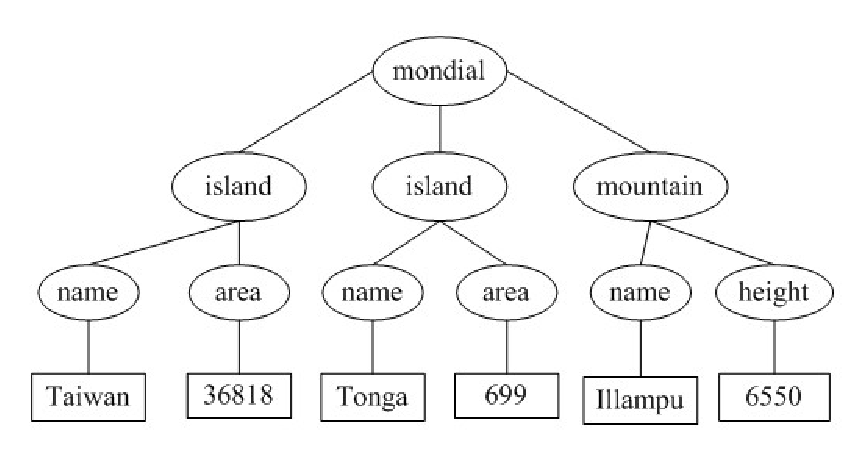
\includegraphics[width=0.4\textwidth]{XML}
\caption{树状结构}\label{fig:xml}
\vspace{\baselineskip}
\end{figure}


其插入图片的代码及其说明如下。
\vspace{1em}\noindent\hrule
\begin{verbatim}
\begin{figure}[H]
\centering
\includegraphics[width=0.4\textwidth]{文件名(.eps)}
\caption{标题}\label{标签名(通常为 fig:labelname)}
\vspace{\baselineskip} %表示图与正文空一行
\end{figure}
\end{verbatim}

\noindent\hrule

\begin{verbatim}
figure环境的可选参数[htbp]表示浮动图形所放置的位置,h (here)表示当前位置,t (top)表示页芯顶部,b (bottom)表示页芯底部,p (page)表示单独一页。在Word等软件中,图片通常插入到当前位置,如果当前页的剩余空间不够,图片将被移动到下一页,当前页就会出现很大的空白,其人工调整工作非常不便。由LaTeX提供的浮动图片功能,总是会按h->t->b->p的次序处理选项中的字母,自动调整图片的位置,大大减轻了工作量。
\centering命令将后续内容转换成每行皆居中的格式。
"\includegraphics"的可选参数用来设置图片插入文中的水平宽度,一般表示为正文宽度(\textwidth)的倍数。
\caption命令可选参数“标签名”为英文形式,一般不以图片或表格的数字顺序作为标签,而应包含一定的图片或表格信息,以便于文中引用(若图片、表格、公式、章节和参考文献等在文中出现的先后顺序发生了变化,其标注序号及其文中引用序号也会跟着发生变化,这一点是Word等软件所不能做到的)。另外,图题或表题并不会因为分页而与图片或表格体分置于两页,章节等各级标题也不会置于某页的最底部,LaTeX系统会自动调整它们在正文中的位置,这也是Word等软件所无法匹敌的。
\vspace将产生一定高度的竖直空白,必选参数为负值表示将后续文字位置向上提升,参数值可自行调整。em为长度单位,相当于大写字母M的宽度。\vspace{\baselineskip} 表示图与正文空一行。
引用方法:“见图~\ref{fig:figname}”、“如图~\ref{fig:figname}~所示”等。
\end{verbatim}

\noindent\hrule\vspace{1em}

若需要将~2~张及以上的图片并排插入到一行中,则需要采用\verb|minipage|环境,如图~\ref{fig:dd}~和图~\ref{fig:ds}~所示。
\begin{figure}[H]
\centering
\begin{minipage}{0.4\textwidth}
\centering
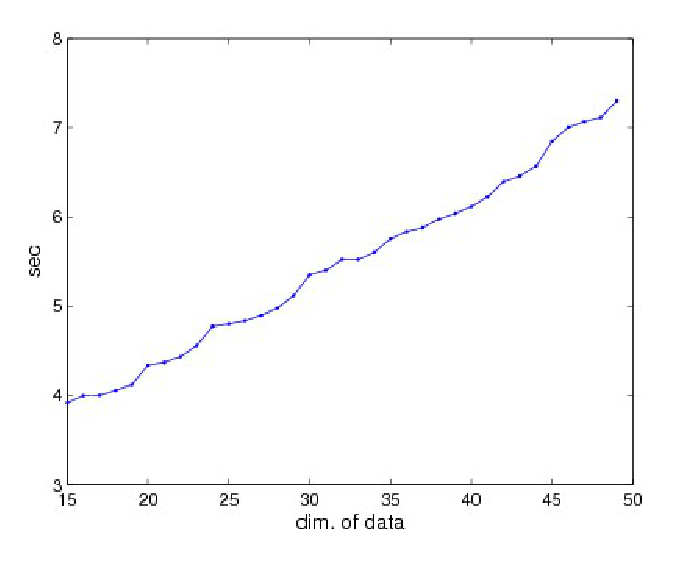
\includegraphics[width=\textwidth]{dataDimensions}
\caption{数据维数的变化}\label{fig:dd}
\end{minipage}
\begin{minipage}{0.4\textwidth}
\centering
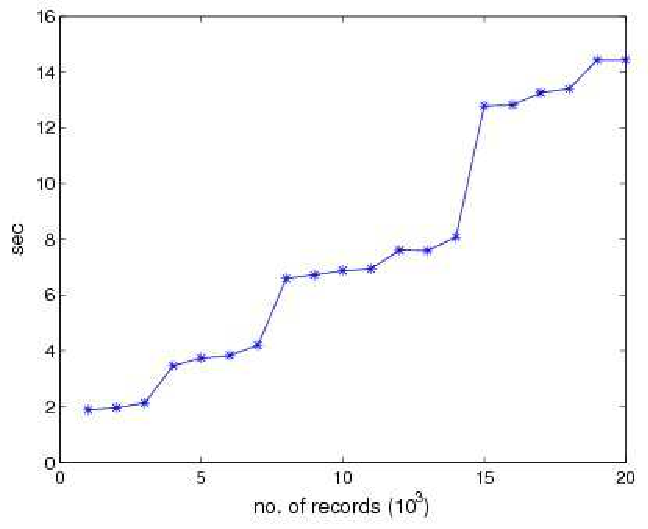
\includegraphics[width=\textwidth]{dataSize}
\caption{数据规模的变化}\label{fig:ds}
\end{minipage}
\vspace{\baselineskip}
\end{figure}

其代码如下所示。
\vspace{1em}\noindent\hrule
\begin{verbatim}
\begin{figure}[H]
\centering
\begin{minipage}{0.4\textwidth}
\centering
\includegraphics[width=\textwidth]{文件名}
\caption{标题}\label{fig:f1}
\end{minipage}
\begin{minipage}{0.4\textwidth}
\centering
\includegraphics[width=\textwidth]{文件名}
\caption{标题}\label{fig:f2}
\end{minipage}\vspace{\baselineskip}
\end{figure}
\end{verbatim}

\noindent\hrule

\begin{verbatim}
minipage环境的必选参数用来设置小页的宽度,若需要在一行中插入n个等宽图片,则每个小页的宽度应略小于(1/n)\textwidth。
\end{verbatim}

\noindent\hrule

\section{具有子图的图片插入方法}

图中若含有子图时,需要调用~subfigure~宏包, 如图~\ref{fig:subfig}~所示。
\begin{figure}[H]
  \centering
  \subfigure[Data Dimensions]{\label{fig:subfig:datadim}
                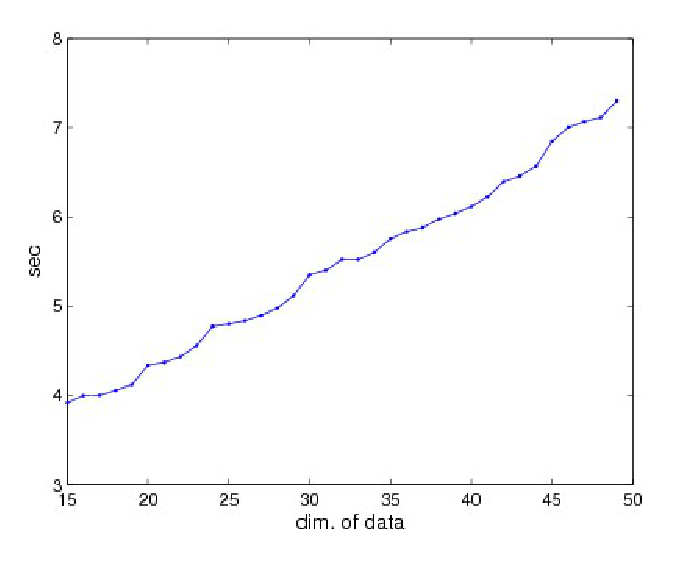
\includegraphics[width=0.4\textwidth]{dataDimensions}}
  \subfigure[Data Size]{\label{fig:subfig:datasize}
                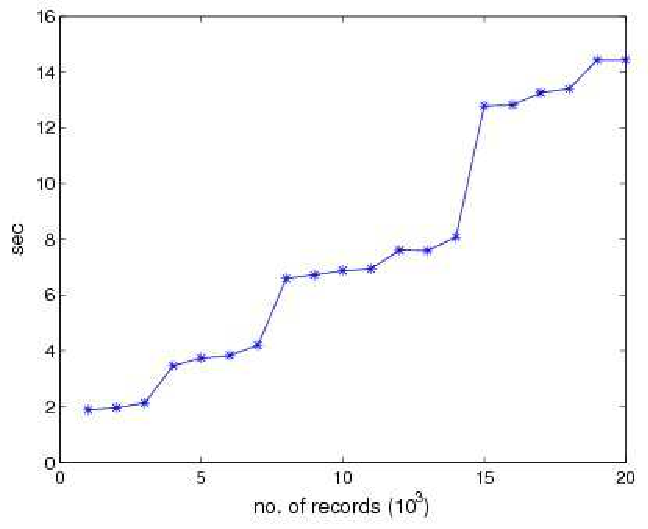
\includegraphics[width=0.4\textwidth]{dataSize}}
  \caption{Scalability of data}\label{fig:subfig}
\vspace{\baselineskip}
\end{figure}

其代码及其说明如下。
\vspace{1em}\noindent\hrule

\begin{verbatim}
\begin{figure}[H]
  \centering
  \subfigure[第1个子图标题]{
            \label{第1个子图标签(通常为 fig:subfig1:subsubfig1)}
            \includegraphics[width=0.4\textwidth]{文件名}}
  \subfigure[第2个子图标题]{
            \label{第2个子图标签(通常为 fig:subfig1:subsubfig2)}
            \includegraphics[width=0.4\textwidth]{文件名}}
  \caption{总标题}\label{总标签(通常为 fig:subfig1)}
\vspace{\baselineskip}
\end{figure}
\end{verbatim}

\noindent\hrule

\begin{verbatim}
子图的标签实际上可以随意设定,只要不重复就行。但为了更好的可读性,我们建议fig:subfig:subsubfig格式命名,这样我们从标签名就可以知道这是一个子图引用。
引用方法:总图的引用方法同本章第1节,子图的引用方法用\ref{fig:subfig:subsubfig}来代替。
\end{verbatim}

\noindent\hrule\vspace{1em}

子图的引用示例:如图~\ref{fig:subfig:datadim}~和图~\ref{fig:subfig:datasize}~所示。

若想获得插图方法的更多信息,参见网络上的~\href{ftp://ftp.tex.ac.uk/tex-archive/info/epslatex.pdf}{Using Imported Graphics in \LaTeX and pdf\LaTeX}~文档。 
%%% !Mode:: "TeX:UTF-8"

\chapter{表格的绘制方法}

\section{本科生毕业设计论文的绘表规范}

表应有自明性。表格不加左、右边线。表的编排建议采用国际通行的三线表。表内中文书写使用宋体五号字。

每个表格之上均应有表题(由表序和表名组成)。表序一般按章编排,如第~1~章第一个插表的序号为“表~1-1”等。表序与表名之间空两格,
表名使用中文五号字,居中。表名中不允许使用标点符号,表名后不加标点。
表头设计应简单明了,尽量不用斜线。表头中可采用化学,物理量等专业符号。

全表如用同一单位,则将单位符号移至表头右上角,加圆括号。
表中数据应准确无误,书写清楚。数字空缺的格内加横线“-”(占~2~个数字宽度)。表内文字或数字上、下或左、右相同时,
采用通栏处理方式,不允许用“〃”、“同上”之类的写法。

表内文字使用宋体五号字,垂直居中书写,起行空一格、转行顶格、句末不加标点。
如某个表需要转页接排,在随后的各页上应重复表的编号。编号后加“(续表)”,表题可省略。续表应重复表头。
表格绘制完成之后,与正文空一行。

\section{普通表格的绘制方法}

表格应具有三线表格式,因此需要调用~booktabs~宏包,其标准格式如表~\ref{tab:table1}~所示。
\begin{table}[htbp]
\caption{符合本科生毕业论文绘图规范的表格}\label{tab:table1}
\vspace{0.5em}\centering\wuhao
\begin{tabular}{ccccc}
\toprule[1.5pt]
$D$(in) & $P_u$(lbs) & $u_u$(in) & $\beta$ & $G_f$(psi.in)\\
\midrule[1pt]
 5 & 269.8 & 0.000674 & 1.79 & 0.04089\\
10 & 421.0 & 0.001035 & 3.59 & 0.04089\\
20 & 640.2 & 0.001565 & 7.18 & 0.04089\\
 5 & 269.8 & 0.000674 & 1.79 & 0.04089\\
10 & 421.0 & 0.001035 & 3.59 & 0.04089\\
20 & 640.2 & 0.001565 & 7.18 & 0.04089\\
 5 & 269.8 & 0.000674 & 1.79 & 0.04089\\
10 & 421.0 & 0.001035 & 3.59 & 0.04089\\
20 & 640.2 & 0.001565 & 7.18 & 0.04089\\
 5 & 269.8 & 0.000674 & 1.79 & 0.04089\\
10 & 421.0 & 0.001035 & 3.59 & 0.04089\\
20 & 640.2 & 0.001565 & 7.18 & 0.04089\\
\bottomrule[1.5pt]
\end{tabular}
\vspace{\baselineskip}
\end{table}

其绘制表格的代码及其说明如下。
\vspace{1em}\noindent\hrule

\begin{verbatim}
\begin{table}[htbp]
\caption{表标题}\label{标签名(通常为 tab:tablename)}
\vspace{0.5em}\centering\wuhao
\begin{tabular}{cc...c}
\toprule[1.5pt]
表头第1个格   & 表头第2个格   & ... & 表头第n个格  \\
\midrule[1pt]
表中数据(1,1) & 表中数据(1,2) & ... & 表中数据(1,n)\\
表中数据(2,1) & 表中数据(2,2) & ... & 表中数据(2,n)\\
表中数据(3,1) & 表中数据(3,2) & ... & 表中数据(3,n)\\
表中数据(4,1) & 表中数据(4,2) & ... & 表中数据(4,n)\\
...................................................\\
表中数据(m,1) & 表中数据(m,2) & ... & 表中数据(m,n)\\
\bottomrule[1.5pt]
\end{tabular}
\vspace{\baselineskip}
\end{table}
\end{verbatim}

\noindent\hrule

\begin{verbatim}
table环境是一个将表格嵌入文本的浮动环境。
\wuhao命令将表格的字号设置为五号字(10.5pt),在绘制表格结束退出时,不需要将字号再改回为\xiaosi,正文字号默认为小四号字(12pt)。
tabular环境的必选参数由每列对应一个格式字符所组成:c表示居中,l表示左对齐,r表示右对齐,其总个数应与表的列数相同。此外,@{文本}可以出现在任意两个上述的列格式之间,其中的文本将被插入每一行的同一位置。表格的各行以\\分隔,同一行的各列则以&分隔。
\toprule、\midrule和\bottomrule三个命令是由booktabs宏包提供的,其中\toprule和\bottomrule分别用来绘制表格的第一条(表格最顶部)和第三条(表格最底部)水平线,\midrule用来绘制第二条(表头之下)水平线,且第一条和第三条水平线的线宽为1.5pt,第二条水平线的线宽为1pt。
引用方法:“如表~\ref{tab:tablename}~所示”。
\end{verbatim}

\noindent\hrule

\section{长表格的绘制方法}

长表格是当表格在当前页排不下而需要转页接排的情况下所采用的一种表格环境。若长表格仍按照普通表格的绘制方法来获得,
其所使用的~\verb|table|~浮动环境无法实现表格的换页接排功能,表格下方过长部分会排在表格第~1~页的页脚以下。为了能够实现长表格的转页接排功能,
需要调用~\verb|longtable|~宏包,由于长表格是跨页的文本内容,因此只需要单独的~\verb|longtable|~环境,所绘制的长表格的格式如表~\ref{tab:table2}~所示。

此长表格~\ref{tab:table2}~第~2~页的标题“编号(续表)”和表头是通过代码自动添加上去的,无需人工添加,若表格在页面中的竖直位置发生了变化,长表格在第~2~页
及之后各页的标题和表头位置能够始终处于各页的最顶部,也无需人工调整,\LaTeX~系统的这一优点是~Word~等软件所无法企及的。

下段内容是为了让下面的长表格分居两页,看到表标题“编号(续表)”的效果。此模板的完成时间正值雨后初霁的四月二十五日,故引用林徽因《你是人间的四月天》全文:
\begin{center}
\begin{minipage}[c]{0.5\textwidth}

\textbf{你是人间的四月天}

\vspace{12pt}
我说你是人间的四月天\\
笑音点亮了四面风\\
轻灵在春的光艳中交舞着变\\
你是四月早天里的云烟\\
黄昏吹着风的软\\
星子在无意中闪\\
细雨点洒在花前\\
那轻~~那娉婷\\
你是鲜妍\\
百花的冠冕你戴着\\
你是天真~~庄严~~你是夜夜的月圆\\
雪化后那片鹅黄\\
你像~~新鲜初放芽的绿\\
你是柔嫩喜悦\\
水光浮动着你梦期待中白莲\\
你是一树一树的花开\\
是燕~~在梁间呢喃\\
你是爱~~是暖\\
是希望\\
你是人间的四月天
\end{minipage}
\end{center}

					
\wuhao\begin{longtable}{cc}
\caption{浙江工业大学各学院名称一览}\label{tab:table2}
 \vspace{0.5em}\\
\toprule[1.5pt] 学院名称 & 网址\\ \midrule[1pt]
\endfirsthead
\multicolumn{2}{c}{表~\thetable(续表)}\vspace{0.5em}\\
\toprule[1.5pt] 学院名称 & 网址\\ \midrule[1pt]
\endhead
\bottomrule[1.5pt]
\endfoot
法学院 & \url{http://www.law.zjut.edu.cn/}\\
化学工程与材料学院 &  \url{http://www.ce.zjut.edu.cn/}\\
机械工程学院 & \url{http://www.jdxy.zjut.edu.cn/}\\
信息工程学院 & \url{http://www.ie.zjut.edu.cn/}\\
计算机科学与技术学院 & \url{http://www.software.zjut.edu.cn/}\\
软件学院 & \url{http://www.software.zjut.edu.cn/}\\
经贸管理学院 & \url{http://www.cba.zjut.edu.cn/}\\
建筑工程学院& \url{http://www.jgxy.zjut.edu.cn/}\\
生物与环境工程学院 & \url{http://www.bee.zjut.edu.cn/}\\
理学院 & \url{http://www.lxy.zjut.edu.cn/}\\
教育科学与技术学院 & \url{http://www.et.zjut.edu.cn/}\\
人文学院 & \url{http://www.rwxy.zjut.edu.cn/}\\
健行学院 & \url{http://www.jxxy.zjut.edu.cn/}\\
外国语学院 & \url{http://www.fl.zjut.edu.cn/}\\
国际学院 & \url{http://www.gjxy.zjut.edu.cn/}\\
政治与公共管理学院 & \url{http://www.sppa.zjut.edu.cn/}\\
艺术学院 & \url{http://www.art.zjut.edu.cn/}\\
药学院 & \url{http://www.yxy.zjut.edu.cn/}\\
成人教育学院 & \url{http://www.cj.zjut.edu.cn/}\\
之江学院 & \url{http://www.zjc.zjut.edu.cn/}\\
研究生院 & \url{http://www.gs.zjut.edu.cn/}\\
\end{longtable}\xiaosi
\vspace{\baselineskip}

绘制长表格的代码及其说明如下。
\vspace{1em}\noindent\hrule

\begin{verbatim}
\wuhao\begin{longtable}{cc...c}
\caption{表标题}\label{标签名(通常为 tab:tablename)}\\
\toprule[1.5pt] 表头第1个格 & 表头第2个格 & ... & 表头第n个格\\ \midrule[1pt]
\endfirsthead
\multicolumn{n}{c}{表~\thetable(续表)}\vspace{0.5em}\\
\toprule[1.5pt] 表头第1个格 & 表头第2个格 & ... & 表头第n个格\\ \midrule[1pt]
\endhead
\bottomrule[1.5pt]
\endfoot
表中数据(1,1) & 表中数据(1,2) & ... & 表中数据(1,n)\\
表中数据(2,1) & 表中数据(2,2) & ... & 表中数据(2,n)\\
...................................................\\
表中数据(m,1) & 表中数据(m,2) & ... & 表中数据(m,n)\\
\end{longtable}\xiaosi
\end{verbatim}

\noindent\hrule
\begin{verbatim}
在绘制长表格的前面留出一个空白行,并在第2行的一开始全局定义长表格的字号为五号字,这样能够保证长表格之前段落的行距保持不变。
在绘制长表格结束后,需要\xiaosi命令重新将字号改为小四号字。
\endhead之前的文字描述的是第2页及其之后各页的标题或表头;
\endfirsthead之前的文字描述的是第1页的标题和表头,若无此命令,则第1页的表头和标题由\endhead命令确定;
同理,\endfoot之前的文字描述的是除最后一页之外每页的表格底部内容;
\endlastfoot之前的文字描述的是最后一页的表格底部内容,若无此命令,
则最后一页的表格底部内容由\endfoot命令确定;由于规范中长表格每页底部内容均相同(水平粗线),因此模板中没有用到\endlastfoot命令。
\end{verbatim}

\noindent\hrule
\section{列宽可调表格的绘制方法}
论文中能用到列宽可调表格的情况共有两种:一种是当插入的表格某一单元格内容过长以至于一行放不下的情况,
另一种是当对公式中首次出现的物理量符号进行注释的情况。这两种情况都需要调用~tabularx~宏包。下面将分别对这两种情况下可调表格的绘制方法进行阐述。
\subsection{表格内某单元格内容过长的情况}

首先给出这种情况下的一个例子如表~\ref{tab:table3}~所示。
\begin{table}[htbp]
\caption{最小的三个正整数的英文表示法}\label{tab:table3}
\vspace{0.5em}\wuhao
\begin{tabularx}{\textwidth}{llX}
\toprule[1.5pt]
Value & Name & Alternate names, and names for sets of the given size\\\midrule[1pt]
1 & One & ace, single, singleton, unary, unit, unity\\
2 & Two & binary, brace, couple, couplet, distich, deuce, double, doubleton, duad, duality, duet, duo, dyad, pair, snake eyes, span, twain, twosome, yoke\\
3 & Three & deuce-ace, leash, set, tercet, ternary, ternion, terzetto, threesome, tierce, trey, triad, trine, trinity, trio, triplet, troika, hat-trick\\\bottomrule[1.5pt]
\end{tabularx}
\vspace{\baselineskip}
\end{table}
绘制这种表格的代码及其说明如下。
\vspace{1em}\noindent\hrule
\begin{verbatim}
\begin{table}[htbp]
\caption{表标题}\label{标签名(通常为 tab:tablename)}
\vspace{0.5em}\wuhao
\begin{tabularx}{\textwidth}{l...X...l}
\toprule[1.5pt]
表头第1个格   & ... & 表头第X个格   & ... & 表头第n个格  \\
\midrule[1pt]
表中数据(1,1) & ... & 表中数据(1,X) & ... & 表中数据(1,n)\\
表中数据(2,1) & ... & 表中数据(2,X) & ... & 表中数据(2,n)\\
.........................................................\\
表中数据(m,1) & ... & 表中数据(m,X) & ... & 表中数据(m,n)\\
\bottomrule[1.5pt]
\end{tabularx}
\vspace{\baselineskip}
\end{table}
\end{verbatim}

\noindent\hrule
\begin{verbatim}
tabularx环境共有两个必选参数:第1个参数用来确定表格的总宽度,这里取为排版表格能达到的最大宽度——正文宽度\textwidth;第2个参数用来确定每列格式,其中标为X的项表示该列的宽度可调,其宽度值由表格总宽度确定。
标为X的列一般选为单元格内容过长而无法置于一行的列,这样使得该列内容能够根据表格总宽度自动分行。若列格式中存在不止一个X项,则这些标为X的列的列宽相同,因此,一般不将内容较短的列设为X。
标为X的列均为左对齐,因此其余列一般选为l(左对齐),这样可使得表格美观,但也可以选为c或r。
\end{verbatim}

\noindent\hrule
\subsection{对物理量符号进行注释的情况}
为使得对公式中物理量符号注释的转行与破折号“———”后第一个字对齐,此处最好采用表格环境。此表格无任何线条,左对齐,
且在破折号处对齐,一共有“式中”二字、物理量符号和注释三列,表格的总宽度可选为文本宽度,因此应该采用\verb|tabularx|环境。
由\verb|tabularx|环境生成的对公式中物理量符号进行注释的公式如式(\ref{eq:1})所示。
%\vspace*{10pt}

\begin{equation}\label{eq:1}
\ddot{\boldsymbol{\rho}}-\frac{\mu}{R_{t}^{3}}\left(3\mathbf{R_{t}}\frac{\mathbf{R_{t}\rho}}{R_{t}^{2}}-\boldsymbol{\rho}\right)=\mathbf{a}
\end{equation}

\begin{tabularx}{\textwidth}{@{}l@{\quad}r@{———}X@{}}
式中& $\bm{\rho}$ &追踪飞行器与目标飞行器之间的相对位置矢量;\\
&  $\bm{\ddot{\rho}}$&追踪飞行器与目标飞行器之间的相对加速度;\\
&  $\mathbf{a}$   &推力所产生的加速度;\\
&  $\mathbf{R_t}$ & 目标飞行器在惯性坐标系中的位置矢量;\\
&  $\omega_{t}$ & 目标飞行器的轨道角速度;\\
&  $\mathbf{g}$ & 重力加速度,$=\frac{\mu}{R_{t}^{3}}\left(
3\mathbf{R_{t}}\frac{\mathbf{R_{t}\rho}}{R_{t}^{2}}-\bm{\rho}\right)=\omega_{t}^{2}\frac{R_{t}}{p}\left(
3\mathbf{R_{t}}\frac{\mathbf{R_{t}\rho}}{R_{t}^{2}}-\bm{\rho}\right)$,这里~$p$~是目标飞行器的轨道半通径。
\end{tabularx}
\vspace{\wordsep}

其中生成注释部分的代码及其说明如下。

\vspace{1em}\noindent\hrule

\begin{verbatim}
\begin{tabularx}{\textwidth}{@{}l@{\quad}r@{— — —}X@{}}
式中 & symbol-1 & symbol-1的注释内容;\\
     & symbol-2 & symbol-2的注释内容;\\
     .............................;\\
     & symbol-m & symbol-m的注释内容。
\end{tabularx}\vspace{\wordsep}
\end{verbatim}

\noindent\hrule

\begin{verbatim}
   tabularx环境的第1个参数选为正文宽度,第2个参数里面各个符号的意义为:
   第1个@{}表示在“式中”二字左侧不插入任何文本,“式中”二字能够在正文中左对齐,若无此项,则“式中”二字左侧会留出一定的空白;
   @{\quad}表示在“式中”和物理量符号间插入一个空铅宽度的空白;
   @{— — —}实现插入破折号的功能,它由三个1/2的中文破折号构成;
   第2个@{}表示在注释内容靠近正文右边界的地方能够实现右对齐。
\end{verbatim}

\noindent\hrule\vspace{1em}

由此方法生成的注释内容应紧邻待注释公式并置于其下方,因此不能将代码放入~\verb|table|~浮动环境中。但此方法不能实现自动转页接排,
可能会在当前页剩余空间不够时,全部移动到下一页而导致当前页出现很大空白。因此在需要转页处理时,还请您手动将需要转页的代码放入一个
新的~\verb|tabularx|~环境中,将原来的一个~\verb|tabularx|~环境拆分为两个~\verb|tabularx|~环境。

若想获得绘制表格的更多信息,参见网络上的~\href{http://www.tug.org/pracjourn/2007-1/mori/}{Tables in \LaTeXe: Packages and Methods}~文档。


%%% !Mode:: "TeX:UTF-8"

\chapter{数学公式的输入方法}
\section{本科生毕业设计论文的公式规范}

论文中的公式应另起行,原则上应居中书写,与周围文字留有足够的空间区分开。
若公式前有文字(如“解”、“假定”等),文字空两格写,公式仍居中写。公式末不加标点。

公式应标注序号,并将序号置于括号内。 公式序号按章编排,如第~1~章第一个公式序号为“(1-1)”。公式的序号右端对齐。

公式较长时最好在等号“=”处转行,如难实现,则可在~$+$、$-$、$\times$、$\div$~运算符号处转行,转行时运算符号仅书写于转行式前,不重复书写。

文中引用公式时,一般用“见式~(1-1)”或“由公式~(1-1)”。

公式中用斜线表示“除”的关系时应采用括号,以免含糊不清,如~$a/(b\cos x)$。通常“乘”的关系在前,如~$a\cos x/b$而不写成~$(a/b)\cos x$。

不能用文字形式表示等式,如:$\textnormal{刚度}=\frac{{\textnormal{受力}}}{{\textnormal{受力方向的位移}}}$。

对于数学公式的输入方法,网络上有一个比较全面权威的文档\textbf{~\href{http://tug.ctan.org/cgi-bin/ctanPackageInformation.py?id=voss-mathmode}{Math mode}}~请大家事先大概浏览一下。下面将对学位论文中主要用到的数学公式排版形式进行阐述。

\section{生成~\LaTeX~数学公式的两种方法}
对于先前没有接触过~\LaTeX~的人来说,编写~\LaTeX~数学公式是一件很繁琐的事,尤其是对复杂的数学公式来说,更可以说是一件难以完成的任务。
实际上,生成~\LaTeX~数学公式有两种较为简便的方法,一种是基于~MathType~数学公式编辑器的方法,另一种是基于~MATLAB~商业数学软件的方法,
下面将分别对这两种数学公式的生成方法作一下简单介绍。

\subsection{基于~MathType~软件的数学公式生成方法}
MathType~是一款功能强大的数学公式编辑器软件,能够用来在文本环境中插入~Windows OLE~图形格式的复杂数学公式,所以应用比较普遍。但此软件只有~30~天的试用期,之后若再继续使用则需要付费购买才行。网络上有很多破解版的~MathType~软件可供下载免费使用,
笔者推荐下载安装版本号在~6.5~之上的中文破解版。

在安装好~MathType~之后,若在输入窗口中编写数学公式,复制到剪贴板上的仍然是图形格式的对象。
若希望得到可插入到~\LaTeX~编辑器中的文本格式对象,则需要对~MathType~软件做一下简单的设置:在~MathType~最上排的按钮中依次选择“参数选项
$\to$转换”,在弹出的对话窗中选中“转换到其它语言(文字):”,在转换下拉框中选择“Tex~--~--~LaTeX 2.09 and later”,并将对话框最下方的两个复选框全部勾掉,点击确定,这样,再从输入窗口中复制出来的对象就是文本格式的了,就可以直接将其粘贴到~\LaTeX~
编辑器中了。按照这种方法生成的数学公式两端分别有标记\verb|\[|和标记\verb|\]|,在这两个标记之间才是真正的数学公式代码。

若希望从~MathType~输入窗口中复制出来的对象为图形格式,则只需再选中“公示对象(Windows OLE~图形)”即可。

\subsection{基于~MATLAB~软件的数学公式生成方法}

MATLAB~是矩阵实验室(Matrix Laboratory)的简称,是美国~MathWorks~公司出品的商业数学软件。它是当今科研领域最常用的应用软件之一,
具有强大的矩阵计算、符号运算和数据可视化功能,是一种简单易用、可扩展的系统开发环境和平台。

MATLAB~中提供了一个~latex~函数,它可将符号表达式转化为~\LaTeX~数学公式的形式。其语法形式为~latex(s),其中,~s~为符号表达式,
之后再将~latex~函数的运算结果直接粘贴到~\LaTeX~编辑器中。从~\LaTeX~数学公式中可以发现,其中可能包含如下符号组合:

\begin{verbatim*}
\qquad=两个空铅(quad)宽度
\quad=一个空铅宽度
\;=5/18空铅宽度
\:=4/18空铅宽度
\,=3/18空铅宽度
\!=-3/18空铅宽度
\ =一个空格
\end{verbatim*}

所以最好将上述符号组合从数学公式中删除,从而使数学公式显得匀称美观。

对于~Word~等软件的使用者来说,在我们通过~MATLAB~运算得到符号表达式形式的运算结果时,在~Word~中插入运算结果需要借助于~MathType~软件,
通过在~MathType~中输入和~MATLAB~运算结果相对应的数学表达形式,之后再将~MathType~数学表达式转换为图形格式粘贴到~Word~中。实际上,
也可以将~MATLAB~中采用~latex~函数运行的结果直接粘贴到~MathType~中,再继续上述步骤,这样可以大大节省输入公式所需要的时间。
此方法在~MathType~6.5c~上验证通过,若您粘入到~MathType~中的仍然为从~MATLAB~中导入的代码,请您更新~MathType~软件。

\section{数学字体}
在数学模式下,常用的数学字体命令有如下几种:

\begin{verbatim}
\mathnormal或无命令 用数学字体打印文本;
\mathit             用斜体(\itshape)打印文本;
\mathbf             用粗体(\bfseries)打印文本;
\mathrm             用罗马体(\rmfamily)打印文本;
\mathsf             用无衬线字体(\sffamily)打印文本;
\mathtt             用打印机字体(\ttfamily)打印文本;
\mathcal            用书写体打印文本;
\end{verbatim}

在学位论文撰写中,只需要用到上面提到的~\verb|\mathit|、\verb|\mathbf|~和~\verb|\mathrm|~命令。若要得到~Times New Roman~的数学字体,则需要调用~txfonts~宏包(此宏包实际上采用的是~Nimbus Roman No9 L~字体,
它是开源系统中使用的免费字体,其字符字体与~Times New Roman~字体几乎完全相同);若要得到粗体数学字体,则需要调用~bm~宏包。表~\ref{tab:fonts}~中分别列出了得到阿拉伯数字、拉丁字母和希腊字母
各种数学字体的命令。

\begin{table}[htbp]
\caption{常用数学字体命令一览}\label{tab:fonts}
\vspace{0.5em}\centering\wuhao
\begin{tabular}{llll}
\toprule
 & 阿拉伯数字\&大写希腊字母 & 大小写拉丁字母 & 小写希腊字母  \\
\midrule
斜体 & \verb|\mathit{}| & \verb|无命令| & \verb|无命令|\\
粗斜体 & \verb|\bm{\mathit{}}| & \verb|\bm{}| & \verb|\bm{}|\\
直立体 & \verb|无命令| & \verb|\mathrm{}| & \verb|字母后加up|\\
粗体 & \verb|\mathbf{}或\bm{}| & \verb|\mathbf{}| & \verb|\bm{字母后加up}|\\
\bottomrule
\end{tabular}
\vspace{\baselineskip}
\end{table}

\noindent 下面列出了一些应采用直立数学字体的数学常数和数学符号。

\section{行内公式}
出现在正文一行之内的公式称为行内公式,例如~$f(x)=\int_{a}^{b}\frac{\sin{x}}{x}dx$。对于非矩阵和非多行形式的行内公式,一般不会使得行距发生变化,而~Word~等软件却会根据行内公式的竖直距离而自动调节行距,如图~\ref{fig:hangju}~所示。

\begin{figure}[htbp]
\centering
\subfigure[由~\LaTeX~系统生成的行内公式]{\label{fig:subfig:latex}
                \fbox{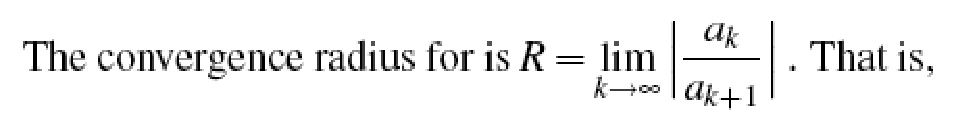
\includegraphics[width=0.55\textwidth]{latex}}}
\subfigure[由~Word软件生成的~.doc~格式行内公式]{\label{fig:subfig:word}
                \fbox{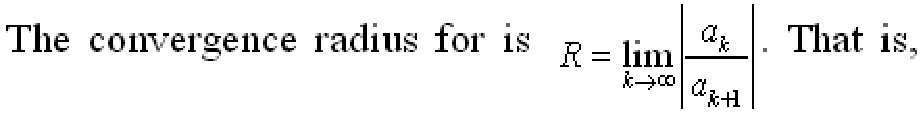
\includegraphics[width=0.55\textwidth]{word}}}
\subfigure[由~Word软件生成的~.pdf~格式行内公式]{\label{fig:subfig:pdf}
                \fbox{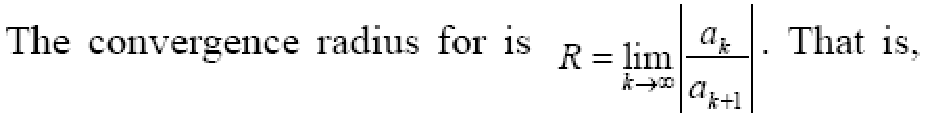
\includegraphics[width=0.55\textwidth]{pdf}}}

\caption{由~\LaTeX~和~Word~生成的~3~种行内公式屏显效果}\label{fig:hangju}
\vspace{-1em}
\end{figure}

这三幅图分别为~\LaTeX~和~Word~生成的行内公式屏显效果,从图中可看出,在~\LaTeX~文本含有公式的行内,在正文与公式之间对接工整,行距不变;而在~Word~文本含有公式的行内,在正文与公式之间对接不齐,行距变大。因此从这一点来说,
\LaTeX~系统在数学公式的排版上具有很大优势。

\LaTeX~提供的行内公式最简单、最有效的方法是采用~\TeX~本来的标记———开始和结束标记都写作~\$,例如本段开始的例子可由下面的输入得到。
\verb|$f(x)=\int_{a}^{b}\frac{\sin{x}}{x}\mathrm{d}x$|

\section{行间公式}
位于两行之间的公式称为行间公式,每个公式都是一个单独的段落,例如
\[\int_a^b{f\left(x\right)dx}=\lim_{\left\|\Delta{x_i}\right\|\to 0}\sum_i{f\left(\xi_i\right)\Delta{x_i}}\]
除人工编号外,\LaTeX~各种类型行间公式的标记见表~\ref{tab:eqtag}。
\begin{table}[htbp]
\caption{各种类型行间公式的标记}\label{tab:eqtag}
\vspace{0.5em}\centering\wuhao
\begin{tabularx}{\textwidth}{cll}
\toprule
& 无编号 & 自动编号\\
\midrule
单行公式& \verb|\begin{displaymath}... \end{displaymath}|& \verb|\begin{equation}... \end{equation}|\\
        & 或~\verb|\[...\]| & \\
多行公式& \verb|\begin{eqnarray*}... \end{eqnarray*}|& \verb|\begin{eqnarray}... \end{eqnarray}|\\
\bottomrule
\end{tabularx}
\end{table}

另外,在自动编号的某行公式行尾添加标签~\verb|\nonumber|,可将该行转换为无编号形式。

行间多行公式需采用~\verb|eqnarray|~或~\verb|eqnarray*|~环境,它默认是一个列格式为~\verb|rcl|~的~3~列矩阵,并且中间列的字号要小一些,因此通常只将需要对齐的运算符号(通常为等号“=”)置于中间列。

\section{可自动调整大小的定界符}
若在左右两个定界符之前分别添加命令~\verb|\left|~和~\verb|\right|,则定界符可根据所包围公式大小自动调整其尺寸,这可从式(\ref{nodelimiter})和式(\ref{delimiter})中看出。
\begin{equation}\label{nodelimiter}
(\sum_{k=\frac12}^{N^2})
\end{equation}
\begin{equation}\label{delimiter}
\left(\sum_{k=\frac12}^{N^2}\right)
\end{equation}
式(\ref{nodelimiter})和式(\ref{delimiter})是在~\LaTeX~中分别输入如下代码得到的。
\begin{verbatim}
(\sum_{k=\frac12}^{N^2})
\left(\sum_{k=\frac12}^{N^2}\right)
\end{verbatim}
\verb|\left|~和~\verb|\right|~总是成对出现的,若只需在公式一侧有可自动调整大小的定界符,则只要用“.”代替另一侧那个无需打印出来的定界符即可。

若想获得关于此部分内容的更多信息,可参见~\href{http://tug.ctan.org/cgi-bin/ctanPackageInformation.py?id=voss-mathmode}{Math mode}~文档的第~8~章“Brackets, braces and parentheses”。

\section{数学重音符号}
数学重音符号通常用来区分同一字母表示的不同变量,输入方法如下(需要调用~\verb|amsmath|~宏包):

\vspace{0.5em}{\noindent\wuhao\begin{tabularx}{\textwidth}{Xc|Xc|Xc}
 \verb|\acute| & $\acute{a}$ & \verb|\mathring| & $\mathring{a}$ & \verb|\underbrace| & $\underbrace{a}$ \\
 \verb|\bar| & $\bar{a}$ & \verb|\overbrace| & $\overbrace{a}$ & \verb|\underleftarrow| & $\underleftarrow{a}$ \\
 \verb|\breve| & $\breve{a}$ & \verb|\overleftarrow| & $\overleftarrow{a}$ & \verb|\underleftrightarrow| & $\underleftrightarrow{a}$ \\
 \verb|\check| & $\check{a}$ & \verb|\overleftrightarrow| & $\overleftrightarrow{a}$ & \verb|\underline| & $\underline{a}$ \\
 \verb|\dddot| & $\dddot{a}$ & \verb|\overline| & $\overline{a}$ & \verb|\underrightarrow| & $\underrightarrow{a}$ \\
 \verb|\ddot| & $\ddot{a}$ & \verb|\overrightarrow| & $\overrightarrow{a}$ & \verb|\vec| & $\vec{a}$ \\
 \verb|\dot| & $\dot{a}$ & \verb|\tilde| & $\tilde{a}$ & \verb|\widehat| & $\widehat{a}$ \\
 \verb|\grave| & $\grave{a}$ & \verb|\underbar| & $\underbar{a}$ & \verb|\widetilde| & $\widetilde{a}$ \\
 \verb|\hat| & $\hat{a}$
\end{tabularx}}\vspace{0.5em}
当需要在字母~$i$~和~$j$~的上方添加重音符号时,为了去掉这两个字母顶上的小点,这两个字母应该分别改用~\verb|\imath|~和~\verb|\jmath|。

如果遇到某些符号不知道该采用什么命令能输出它时,则可通过~\href{http://detexify.kirelabs.org/classify.html}{Detexify$^2$~网站}来获取符号命令。若用鼠标左键在此网页的方框区域内画出你所要找的符号形状,则会在网页右方列出和你所画符号形状相近的~5~个符号及其相对应的~\LaTeX~输入命令。若所列出的符号中不包括你所要找的符号,还可通过点击“Select from the complete list!”的链接以得分从低到高的顺序列出所有符号及其相对应的~\LaTeX~输入命令。

最后,建议大家还以~\href{http://tug.ctan.org/cgi-bin/ctanPackageInformation.py?id=voss-mathmode}{Math mode}~这篇~pdf~文档作为主要参考。若要获得最为标准、美观的数学公式排版形式,可以查查文档中是否有和你所要的排版形式相同或相近的代码段,通过修改代码段以获得你所要的数学公式排版形式。


%%% !Mode:: "TeX:UTF-8"

\chapter{罗列、定理和代码环境使用方法}

\section{单层罗列环境}

浙江工业大学毕业设计论文一般可采用两种罗列环境:一种是并列条目有同样标签的~\verb|itemize|~罗列环境,另一种是具有自动排序编号符号的~\verb|enumerate|~罗列环境。这两种罗列环境的样式参数可参考图~\ref{fig:list}。
\begin{figure}[htbp]
\centering
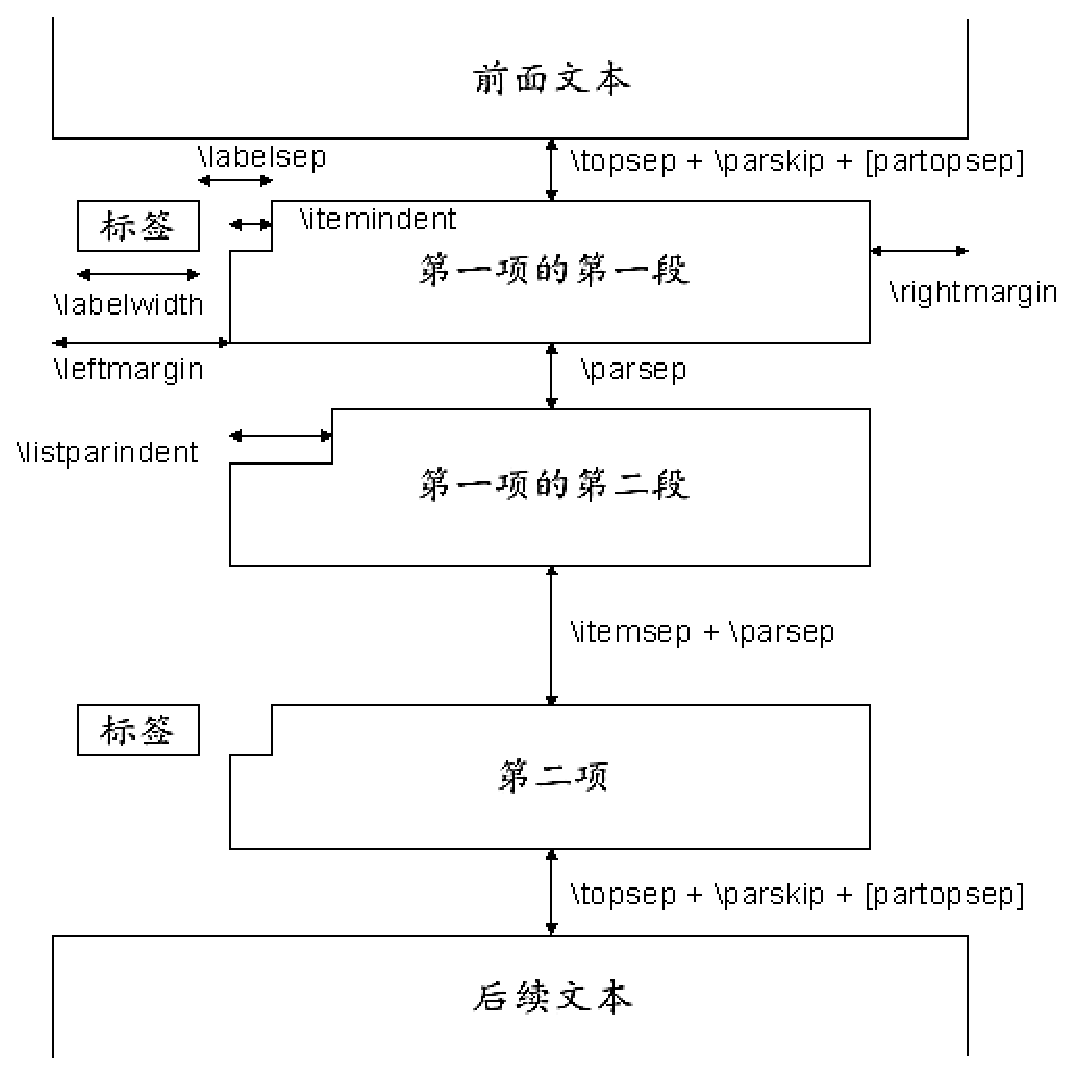
\includegraphics[width = 0.6\textwidth]{list}
\caption{罗列环境参数示意图}\label{fig:list}\vspace{-1em}
\end{figure}

通过调用~enumitem~宏包可以很方便地控制罗列环境的布局,其~format.tex~文件中的~\verb|\setitemize|~和~\verb|\setenumerate|~命令分别用来设置~\verb|itemize|~和~\verb|enumerate|~环境的样式参数。采用~\verb|itemize|~单层罗列环境的排版形式如下:

\begin{itemize}
\item 第一个条目文本内容
\item 第二个条目文本内容
\item 第三个条目文本内容
\end{itemize}

其代码如下

\begin{verbatim}
\begin{itemize}
  \item 第一个条目文本内容
  \item 第二个条目文本内容
  ...
  \item 第三个条目文本内容
\end{itemize}
\end{verbatim}

采用~\verb|enumerate|~单层罗列环境的排版形式如下:

\begin{enumerate}
\item 第一个条目文本内容
\item 第二个条目文本内容
\item 第三个条目文本内容
\end{enumerate}

其代码如下

\begin{verbatim}
\begin{enumerate}
  \item 第一个条目文本内容
  \item 第二个条目文本内容
  ...
  \item 第三个条目文本内容
\end{enumerate}
\end{verbatim}



\section{定理环境}

\begin{definition}[谱半径]\label{def:def1}
  称~$n$~阶方阵~$\mathbf{A}$~的全体特征值~$\lambda_1,\cdots,\lambda_n$~组成的集合为~$\mathbf{A}$~的谱,称
  $$\rho(\mathbf{A})=\max{\{|\lambda_1|,\cdots,|\lambda_n|\}}$$
\end{definition}
\begin{theorem}[相似充要条件]\label{lemma:l1}
  方阵$A$和$B$相似的充要条件是:~$A$~和~$B$~有全同的不变因子。
\end{theorem}
\begin{corollary}[推论1]\label{cor:cor1}
在赋范空间~$(X,\|\cdot\|)$~上定义~$d(x,y)=\|x-y\|$, 对任意~$x,y\in X$,~则~$(X,d)$~是距离空间。
\end{corollary}
\begin{proof}
  只需证明~$d(x,y)$~是距离。
\end{proof}
\newpage

定义代码如下:
\begin{verbatim}
 \begin{definition}[谱半径]\label{def:def1}
  称~$n$~阶方阵~$\mathbf{A}$~的全体特征值
  $\lambda_1,\cdots,\lambda_n$组成的集合为~$\mathbf{A}$~的谱,称
  $$\rho(\mathbf{A})=\max{\{|\lambda_1|,\cdots,|\lambda_n|\}}$$
\end{definition}
\end{verbatim}
\noindent\hrule

\vspace{0.1em}\noindent\hrule
\vspace{1em}
定理代码如下:
\begin{verbatim}
\begin{theorem}[相似充要条件]\label{lemma:l1}
  方阵$A$和$B$相似的充要条件是:$A$和$B$有全同的不变因子。
\end{theorem}
\end{verbatim}

\noindent\hrule\vspace{0.1em}

\noindent\hrule
\vspace{1em}
推论和证明代码如下:
\begin{verbatim}
\begin{corollary}[推论1]\label{cor:cor1}
在赋范空间~$(X,\|\cdot\|)$~上定义$d(x,y)=\|x-y\|$,
对任意$x,y\in X$,则$(X,d)$是距离空间。
\end{corollary}
\begin{proof}
  只需证明$d(x,y)$是距离。
\end{proof}
\end{verbatim}
\noindent\hrule\vspace{1em}

定理定义[]中是可选参数,用来说明定理的名称。其他环境格式书写与上面定理、定义、推论格式相同,可自己调用其他环境。
若需要书写定理定义等内容,而且带有顺序编号,需要采用如下环境。除了~\verb|proof|~环境之外,其余~9~个环境都可以有一个可选参数作为附加标题。

\begin{center}
\vspace{0.5em}\noindent\wuhao\begin{tabularx}{0.7\textwidth}{lX|lX}
定理 & \verb|theorem|~环境 & 定义 & \verb|definition|~环境 \\
例 & \verb|example|~环境 & 算法 & \verb|algorithm|~环境 \\
公理 & \verb|axiom|~环境 & 命题 & \verb|proposition|~环境 \\
引理 & \verb|lemma|~环境 & 推论 & \verb|corollary|~环境 \\
注解 & \verb|remark|~环境 & 证明 & \verb|proof|~环境 \\
\end{tabularx}
\end{center}
\section{代码环境}
很多和计算机专业背景相关的同学都会使用到代码环境,使用~\verb|\verb|~指令或者是~\verb|verbatim|~环境固然是一种选择,但是比不上专门的~lstlisting~环境这么专业。
\begin{lstlisting}[language=C]
int main(int argc, char ** argv)
{
	printf("Hello world!\n");
	return 0;
}
\end{lstlisting}

\noindent\hrule
\vspace{0.1em}\noindent\hrule

\vspace{1em}

\noindent 代码如下:
\begin{verbatim}
\begin{lstlisting}[language=C]
int main(int argc, char ** argv)
{
	printf("Hello world!\n");
	return 0;
}
\end{lstlisting}
\end{verbatim}
\noindent\hrule\vspace{1em}

在代码中显示的关键字为蓝色,框的左侧显示的是行号,这样便于读者阅读和查找代码,同时添加了浅蓝色的阴影边框,达到了美观的效果。
代码环境的设置已在~package~中~\verb|\lstset|~指令中定义。定义中支持跨页显示,可以将较长的代码置于~lstlisting~环境中。
\section{算法环境}
很多和计算机专业背景相关的同学会使用到算法环境,之前使用到的定理环境固然是一种选择,但是比不上专门的~algorithm2e~环境这么专业。为了实现专业和接近完美,本版本支持算法环境。如下所示:
\begin{algorithm}[htbp]
    \caption{算法标题}
    \label{alg:demoAlgo} % 贴上标签以便交叉引用
    \begin{algorithmic}[1]  % 这个 1 表示每一行都显示数字
    \STATE 初始化...
    \FOR{$i=0;i\le M; i\rightarrow i + 1$}
        \STATE 执行语句~1;
        \STATE 执行语句~2;
        \STATE ...
    \ENDFOR
    \STATE ...
    \WHILE{某条件}
        \STATE 执行语句~1;
        \STATE 执行语句~2;
        \STATE ...
    \ENDWHILE
    \STATE ...
    \end{algorithmic}
\end{algorithm}
\noindent\hrule
\vspace{0.1em}\noindent\hrule

\vspace{1em}

\noindent 代码如下:
\begin{verbatim}
  \begin{algorithm}[htbp]
    \caption{算法标题}
    \label{alg:demoAlgo} % 贴上标签以便交叉引用
    \begin{algorithmic}[1]  % 这个 1 表示每一行都显示数字
    \STATE 初始化...
    \FOR{$i=0;i\le M; i\rightarrow i + 1$}
        \STATE 执行语句~1;
        \STATE 执行语句~2;
        \STATE ...
    \ENDFOR
    \STATE ...
    \WHILE{某条件}
        \STATE 执行语句~1;
        \STATE 执行语句~2;
        \STATE ...
    \ENDWHILE
    \STATE ...
    \end{algorithmic}
\end{algorithm}
\end{verbatim}


%%% !Mode:: "TeX:UTF-8"

\chapter{总结与展望}
随着我国高等教育规模的不断扩大,教学质量的不断提高,研究项目的不断增多,信息化程不断增高,基于互联网的项目申报系统将日益受到重视[27]。传统的纸质项目申报评审方式面临着很大的挑战,迫切要求我们实现项目申报评审的科学化、现代化。对此,网上项目申报评审系统的开发日益迫切,项目的开发意义也越来越重要。

	“浙江省教育厅教育质量与教学改革项目申报管理系统”是一个集项目信息发布、项目管理、项目网上申报评审管和项目成果展示为一体的信息化管理系统。为用户提供一个方便、快捷、透明、高效的项目申报评审环境。系统的实现将有效的提高项目主管部门、学校、老师的工作效率,带来巨大的经济效益。

\end{verbatim}
那么,编译的时候就只编译未加~\%~的一章,在这个例子中,即本章~intros。

理论上,并不一定要把每章放在不同的文件中。但是这种自顶向下,分章节写作、编译的方法有利于提高效率,大大减少~Debug~过程中的编译时间,同时减小风险。

\section{参考文献生成方法}

\LaTeX~具有插入参考文献的能力。Google Scholar~网站上存在兼容~BibTeX~的参考文献信息,通过以下几个步骤,可以轻松完成参考文献的生成。
\begin{itemize}
  \item 在\href{http://scholar.google.com/}{谷歌学术搜索}中,
        点击\href{http://scholar.google.com/scholar_preferences?hl=en&as_sdt=0,5}{学术搜索设置}。
  \item 页面打开之后,在\textbf{文献管理软件}选项中选择\textbf{显示导入~BibTeX~的链接},单击保存设置,退出。
  \item 在谷歌学术搜索中检索到文献后,在文献条目区域单击导入~BibTeX~选项,页面中出现文献的引用信息。
  \item 将文献引用信息的内容复制之后,添加到~references~文件夹下的~reference.bib~中。
\end{itemize}

\section{编译注意事项}
\begin{enumerate}
  \item 由于模板使用~UTF-8~编码,所以源文件应该保存成~UTF-8~格式,否则可能出现中文字符无法识别的错误。
  本模板中每一个~.tex~文件的文件的开头已经加上一行:\\
  \verb|% !Mode:: "TeX:UTF-8"|\\
     这样可以确保~.tex~文件默认使用~UTF-8~的格式打开。读者如果删去此行,很有可能会导致中文字符显示乱码。
     在~WinEdt~编辑器中可以使用以下两种方式保存成~UTF-8~格式:
      \begin{enumerate}
        \item 先建立~.tex~文件,另存为~.tex~文件时,选择用~UTF-8~格式保存。
        \item
            在~WinEdt~编辑器中,选择\\
            \mbox{~Document$\to$Document Settings$\to$Document Mode $\to$TeX:UTF-8} 同时在\\~WinEdt~最下面的状态栏中,可以看到该文档是~TeX~格式还是~TeX:UTF-8~格式。
            当文档为~TeX:UTF-8~格式时,状态栏一般显示:\\
            \makebox[\textwidth][l]{Wrap | Indent | INS | LINE |Spell | TeX:UTF-8 | -src~等。}
      \end{enumerate}
  \item 如果在pdf书签中,中文显示乱码的话,则注意以下说明:
    \begin{verbatim}
        \usepackage{CJKutf8}
        % 1. 如果使用CJKutf8
        %    Hyperref中应使用unicode参数
        % 2. 如果使用CJK
        %    Hyperref则使用CJKbookmarks参数
        %    可惜得到的PDF书签是乱码,建议弃用
        % 3. Unicode选项和CJKbookmarks不能同时使用
        \usepackage[
        %CJKbookmarks=true,
        unicode=true
        ]{hyperref}
     \end{verbatim}
  \item 建议采用以下两种编译方式:
  \begin{enumerate}
    \item xelatex + bibtex + xelatex + xelatex, 在这种编译情况下,所有图片文件应该保存成~.eps~格式,如~figures~文件夹里~.eps~图片。
  \end{enumerate}
\end{enumerate}

\section{系统要求}
    CTEX 2.8, MiKTeX 2.8 或者 TeX Live 2009。使用推荐的~WinEdt 6.0~编辑器,可以完成文件的编辑和编译工作。

\section{\TeX~简介}

以下内容是~milksea@bbs.ctex.org~撰写的关于~\TeX~的简单介绍,略有改动。
注意这不是一个入门教程,不讲~\TeX~系统的配置安装,也不讲具体的~\XeLaTeX~代码。
这里仅仅试图以一些只言片语来解释:
进入这个门槛之前新手应该知道的注意事项,以及遇到问题以后该去如何解决问题。

\subsection{什么是 \TeX/\XeLaTeX,我是否应该选择它~?}

\TeX~是最早由高德纳(Donald Knuth)教授创建的一门标记式宏语言,
用来排版科技文章,尤其擅长处理复杂的数学公式。\TeX~同时也是处理这一语言的排版软件。
\XeLaTeX~是 Leslie Lamport 在~\TeX~基础上按内容/格式分离和模块化等思想建立的一集~\TeX~上的格式。

\TeX~本身的领域是专业排版领域
但现在~TeX/LaTeX~也被广泛用于生成电子文档甚至幻灯片等,~\TeX~语言的数学部分
偶尔也在其他一些地方使用。但注意~\TeX~并不适用于文书处理(Microsoft Office 的领域,以前和现在都不是)。

选择使用~\TeX/\XeLaTeX~的理由包括:
\begin{itemize}
\item 免费软件;
\item 专业的排版效果;
\item 是事实上的专业数学排版标准;
\item 广泛的西文期刊接收甚或只接收 LaTeX 格式的投稿;
\item[] ……
\end{itemize}
不选择使用~\TeX/\XeLaTeX~的理由包括:
\begin{itemize}
\item 需要相当精力学习;
\item 图文混合排版能力不够强;
\item 仅在数学、物理、计算机等领域流行;
\item 中文期刊的支持较差;
\item[] ……
\end{itemize}

请尽量清醒看待网上经常见到的关于~\TeX~与其他软件的优劣比较和口水战。在选择使用或离开之前,请先考虑
\TeX~的应用领域,想想它是否适合你的需要。


\subsection{我该用什么编辑器~?}

编辑器功能有简有繁,特色不一,从简单的纯文本编辑器到繁复的 Emacs,因人而易。基本功能有语法高亮、方便编译预览就很好了,扩充功能和定制有无限的可能。初学者可以使用功能简单、使用方便的专用编辑器,如 ~TeXWorks、Kile、WinEdt~等,或者类似所见即所得功能的~LyX;熟悉的人可以使用定制性更强的~Notepad++、SciTE、Vim、Emacs ~等。这方面的介绍很多,一开始不妨多试几种,找到最适合自己的才是最好的。

另外提醒一句,编辑器只是工作的助手,不必把它看得太重。

\subsection{我应该看什么~\XeLaTeX~读物~?}

这不是一个容易回答的问题,因为有许多选择,也同样有许多不合适的选择。
这里只是选出一个比较好的答案。更多更详细的介绍可以在版面和网上寻找(注意时效)。

近两年~\TeX~的中文处理发展很快,目前没有哪本书在中文处理方面给出一个最新进展的合适综述,
因而下面的介绍也不主要考虑中文处理。

\begin{enumerate}

\item 我能阅读英文。
\begin{enumerate}
\item 迅速入门:ltxprimer.pdf (LaTeX Tutorials: A Primer, India TUG)
\item 系统学习:A Guide to LaTeX, 4th Edition, Addison-Wesley
               有机械工业出版社的影印版(《\LaTeX{}~实用教程》)
\item 深入学习:要读许多书和文档,TeXbook 是必读的
\item 细节学习:去读你使用的每一个宏包的说明文档
\item 专题学习:阅读讲数学公式、图形、表格、字体等的专题文档
\end{enumerate}

\item 我更愿意阅读中文。
\begin{enumerate}
\item 迅速入门:lnotes.pdf (LaTeX Notes, 1.20, Alpha Huang)
\item 系统学习:《\LaTeXe{}~科技排版指南》,邓建松(电子版)
      如果不好找,可以阅读《\LaTeXe~入门与提高》第二版,陈志杰等,或者 《\LaTeXe~完全学习手册》,胡伟
\item 深入学习:~TeXbook0.pdf~(特可爱原本,TeXbook 的中译,xianxian)
\item 具体问题释疑:~CTeX-FAQ.pdf~,\\
        吴凌云,~\url{http://www.ctex.org/CTeXFAQ}~
\end{enumerate}
\end{enumerate}

遇见问题和解决问题的过程可以快速提高自己的技能,建议此时:
\begin{itemize}
  \item 利用~Google~搜索。
  \item 清楚,扼要地提出你的问题。
\end{itemize}

\subsection{什么知识会过时~?什么不会~?}

\TeX~是排版语言,也是广泛使用的软件,并且不断在发展中;
因此,总有一些东西会很快过时。作为学习~\TeX~的人,
免不了要看各种各样的书籍、电子文档和网络论坛上的只言片语,
因此了解什么知识会迅速过时,什么知识不会是十分重要的。

最稳定的是关于~Primitive \TeX~和~Plain \TeX~的知识,也就是 Knuth
在他的《The TeXbook》中介绍的内容。因为~\TeX~
系统开发的初衷就是稳定性,要求今天的文档到很久以后仍可以得到完全相同的结果,
因此 Knuth 限定了他的~\TeX~语言和相关实现的命令、语法。这些内容许多年来就没有多少变化,
在未来的一些年里也不会有什么变化。
Primitive \TeX~和 Plain \TeX~的知识主要包括 \TeX~排版的基本算法和原理,
盒子的原理,底层的 \TeX~命令等。其中技巧性的东西大多在宏包设计中,
初学者一般不会接触到很多;而基本原理则是常常被提到的,
譬如,~\TeX~把一切排版内容作为盒子(box)处理。

相对稳定的是关于基本~\LaTeXe~
的知识,也包括围绕~\LaTeXe~的一些核心宏包的知识。
在可预见的将来,~\LaTeXe~不会过时。
\LaTeXe~的知识是目前大部分~\LaTeX~书籍的主体内容。关于~\XeLaTeX~的标准文档类
~(article、report、book、letter、slide~等),关于基本数学公式的输入,
文档的章节层次,表格和矩阵,图表浮动体,LR 盒子与段落盒子……
这些~\XeLaTeX~的核心内容都是最常用的,相对稳定的。
与~\LaTeXe~相匹配的核心宏包,
如~graphics(x)、ifthen、fontenc、doc~等,也同样是相对稳定的。
还有一些被非常广泛应用的宏包,如~amsmath~系列,也可以看作是相对稳定的。

简单地说,关于基本~\TeX/\XeLaTeX~的语言,都是比较稳定的。与之对应,实现或者支持~\TeX/\XeLaTeX~语言的软件,
包括在~\TeX/\XeLaTeX~基础上建立的新的宏,都不大稳定。

容易过时的是关于第三方~\XeLaTeX~宏包的知识、第三方~\TeX~工具的知识,以及新兴~\TeX~相关软件的知识等。
~\TeX~和~\XeLaTeX~语言是追求稳定的;但无论是宏包还是工具,作为不断更新软件,它们是不稳定的。
容易过时的技术很多,而且现在广泛地出现在几乎所有~\XeLaTeX~文档之中,因此需要特别引起注意:
宏包的过时的原因可能是宏包本身的升级换代带来了新功能或不兼容,
也可能是同一功能的更新更好的宏包代替了旧的宏包。前者的典型例子比如绘图宏包~PGF/TikZ~,
现在的~2.00~版功能十分强大,和旧的~1.1x~版相差很大,和更旧的~0.x~版本则几乎完全不同;后
者的典型例子比如~caption~宏包先是被更新的~caption2~宏包代替,后来~caption~宏包更新又使得
caption2 宏包完全过时。——安装更新的发行版可以避免使用过旧的宏包;
认真阅读宏包自带的文档而不是搜索得到的陈旧片断可以避免采用过时的代码。

工具过时的主要原因也是升级换代和被其他工具替换。前者的典型例子是编辑器
WinEdt~在~5.5~以后的版本支持~UTF-8~编码,而旧版本不支持;
后者的典型例子是中文字体安装工具从~GBKFonts~到~xGBKFonts~到~FontsGen~不断被取代。
图形插入是一个在~\TeX~实现、宏包与外围工具方面都更新很快的东西。
在过去,最常用的输出格式是~PS(PostScript)~格式,因此插入的图像以~EPS~为主流。
使用~Dvips~为主要输出工具,外围工具有~GhostScript、bmeps~等等,相关宏包有~graphics~等,
相关文档如《\LaTeXe{}~ 插图指南》。

\XeLaTeX~不限定图片格式,推荐使用EPS格式的图片,但是PNG和JPEG格式的图片也支持。

值得特别提出注意的就是,中文处理也一起是更新迅速、容易过时的部分。
而且因为中文处理一直没有一个“官方”的“标准”做法,软件、工具、
文档以及网上纷繁的笔记也就显得相当混乱。从八十年代开始的~CCT~系统、
天元系统,到后来的~CJK~方式,到近来的~XeTeX~和~LuaTeX~ 方式,
中文处理的原理、软件、宏包、配置方式等都在不断变化中。

\section{班级写法}
封面上需填写规范的学科专业和专业班级。专业写法见表~\ref{tab:major}~,班级写法见表~\ref{tab:class}~。可能这里不能顾及到所有专业和班级的写法,同学们可以自行咨询老师,询问自己专业和班级的规范写法。

\begin{table}[H]
\caption{专业写法}\label{tab:major}
\vspace{0.5em}
\begin{center}
{\wuhao
\begin{tabular}{c}
\toprule[1.5pt]
专业写法\\
\midrule[1pt]
计算机科学与技术\\
软件工程\\
数字媒体技术\\
网络工程\\
物联网工程\\
\bottomrule[1.5pt]
\end{tabular}}
\end{center}
\vspace{\baselineskip}
\end{table}

\begin{table}[H]
\caption{班级写法}\label{tab:class}
\vspace{0.5em}
\begin{center}
{\wuhao
\begin{tabular}{cc}
\toprule[1.5pt]
班级写法 & 班级写法\\
\midrule[1pt]
计算机+自动化0901 & 计算机+自动化0902\\
计算机0901 & 计算机0902\\
计算机0903 & 计算机0904\\
软件工程0901 & 软件工程0902\\
软件工程0903 & 软件工程0904\\
软件工程0905 & 软件工程0906\\
软件工程0907 & 软件工程0908\\
数字媒体技术0901 & 数字媒体技术0902\\
网络工程0901 & 网络工程0902\\
软件工程(2+2)1101 & 软件工程(2+2)1102\\
软件工程(2+2)1103 & 软件工程(专升本)1101\\
软件工程(专升本)1102 & 计算机学院实验班1101\\
物联网工程1201 & \\
\bottomrule[1.5pt]
\end{tabular}}
\end{center}
\vspace{\baselineskip}
\end{table}

\section{后期工作}
下表记录了~ZJUTThesis~计划中未来应该逐步实现的功能和特性:
\begin{enumerate}
  \item 编写更为详细的~ZJUTThesis~的使用手册和~FAQ~用户指南
  \item 加入对课程结课论文的支持
  \item 加入对浙江工业大学学生经常参加的各种限时完成重大赛事的论文模板的支持,如美国大学生数学建模竞赛(MCM),以节省排版时间
  \item 加入对~pdf~书签中章节中文编号的支持,如: 第一章 XXX
  \item 加入对附录~A~等格式的支持
  \item Linux~平台迁移和测试
\end{enumerate}

\section{免责声明}

本模板依据《浙江工业大学本科生毕业设计说明书(论文)模板》编写,作者希望能给使用者写作论文带来方便。然而,作者不保证本模板完全符合学校要求,也不对由此带来的风险和损失承担任何责任。

\clearpage
% !Mode:: "TeX:UTF-8"

\chapter{研究意义}
“浙江省教育厅教育质量与教学改革项目申报管理系统”是基于互联网的B/S体系结构系统。它充分利用互联网的硬件、软件资源,实现信息的实时发布、项目的网上申报、网上专家评审、项目成果网上展示。本系统的开发,是进一步推动浙江省信息化进程的一个重要举措。教育乃国家兴旺发达的关键,有一个迅速、敏捷的教学质量工程申报评审管理系统将有效的提高教学质量,本系统的开发无疑是向该方向迈进一大步。建设“浙江省教育厅教学质量与教学改革项目申报管理系统”将能有效地促进高等教育处的管理工作。

% !Mode:: "TeX:UTF-8"

\chapter{国内外研究现状及难点}
在国外,教学质量管理已有90年的历史。以美国为代表的许多国家,如澳大利亚、英国、加拿大、比利时等国都相继采用学生评教来评价教师的教学效果。以美国为例,20世纪70年代初,美国教育委员会的一个调查结果表明,在被调查的669所高等学校中,大约有65%的高校在系一级机构中允许学生对教学进行评价,到80年代以后,学生评教不但成为大学教学评价的二个重要组成部分,且评价技术越来越现代化。目前,许多大学已经开发使用了基于网络的学生评教系统,如华盛顿大学的IAS(Instructional Assessment System)、亚利桑那大学的TCE(Teacher-Course Evaluation)、堪萨斯州立大学的IDEA(Individual Development and Educational Assessment)等[2],这些系统通过校园网络实施教学评价,取得了较好的效果。美国等国家已经有网上申报、网上专家评审的系统,基于网络的申报管理信息系统国外已进入实用研究阶段,大量的投入到各种项目的网上申报、网上评审的实际运用中,提高的项目申报申批的效率,取得了重大的经济效益。

在我国,学生评教的发展经历了定性评教为主和定量评教为主等阶段,比较规范的科学的学生评教活动应当说是伴随科学的高教评估活动的兴起而逐步形成并得到良好发展的。1985年之后开展的各种高教评估试点活动,都离不开对教学质量特别是课堂教学质量的评估,对于后者除了用统测的办法之外,另一个更为可行的办法就是学生评教[4]。我国的学生评教活动始于20世纪80年代初,特别是从1987年起,随着教师职称评定工作日益规范化,许多高校对教师的教学提出了越来越高的要求,学生评教活动开展得越来越普遍。2001年教育部4号文件——《关于加强高等学校本科教学工作提高教学质量的若干意见》出台后,学生评教在全国普通高校更是得到了广泛的开展,评教方式和技术手段也逐步得到了改进。各种基于网络的学生评教信息系统也取得了较大的进展。但相比于国外而言,我国的教学质量网上管理系统的开发还有一定的距离,而且在国家与省级之间也存在着一定的差距。国家教学质量与教学改革工程项目的立项都已经实现网上申报、网上评审,种类科技项目一般也都已经实行网上申报、网上评审。但浙江省高教处的项目管理工作基本上都是基于传统的纸质材料,已经严重落后于电子政务建设的步伐,管理很难全面地了解把握各类建设项目的立项、建设进展等情况。这样既不符合申报材料电子化的趋势,也限制了项目评审专家的选择、项目评审的公平、公正。因此,在国外已进入实用研究阶段时,国内还处于设想开发的初级阶段。

目前,该领域研究的难点主要有:基于互联网申报、评审的管理模式的研究,对于多层次、多级别的管理层,针对复杂多样的网络环境,提出一种适合于互联网的申报、评审管理模式;数据的安全性,对于数据的远程传输、备份及权限的设计、加密算法等;各种网上结构化、非结构化表格的处理与管理,面对不同级别、不同类型的项目立项报告书,格式转换、存储、传输、输出和归档管理,以及查询、修改、分类统计和输出;不同层次的机构组织的通讯、协调管理,有关项目需要主管部门先评审或者主管部门先排序,再上报省教育厅正式评审,而有关项目不需要主管部门先评审可直接报省科技厅评审,这样系统必然对不同项目进行不同级别的管理。

% !Mode:: "TeX:UTF-8"

\chapter{系统通用结构}
本申报系统是一个典型的管理信息系统[5](Management Information System)简称MIS。它是1961年在美国由J.D.Gdllagher首先提出的,并确定其以计算机为主体,信息处理为中心的综合性系统,由计算机技术、网络通讯技术、信息处理技术、管理科学和人组成的一个综合系统,能提供信息以支持一个组织机构的运行、管理和决策功能。

对于典型的MIS系统结构通过主要有三类[6]:\par
工作站、文件服务器结构的MIS系统。这种结构中,应用程序逻辑完全是在客户工作站上执行,一台或多台中央服务器提供了对于计算资源的访问途径。文件服务器只是提供文件访问服务,没有真正意义上的数据库引擎。这样所有程序逻辑均在客户端完成,容易造成客户端负担过重,随着基于客户机、服务器结构MIS的出现,使工作站、文件服务器结构的第一代MIS系统渐渐淡出主流MIS阵营。

C/S结构的MIS系统,这种结构借助于网络将应用资源和应用任务合理的分配到CLINET、SERVER两端。具体的,客户端主要功能是负责人机交互,管理用户接口、执行客户端应用程序,采集数据以及向服务器提交应用请求,而服务器则执行后台程序,主要承担数据库存储系统的共享管理、通讯管理、文件管理以及对客户机的请求提供服务。

B/S结构的MIS系统,这种结构与C/S模式相比,它简化了客户端的程序,通常在这种模式结构的系统中,客户端只需要一个浏览器就可以了。这种结构将许多工作交于WEB服务器来做,客户端只通过浏览器请求WEB服务,WEB服务器再根据不同请求返回信息,这其中还需请求数据库服务器以获取正确数据。因此,这种结构模式的MIS系统,而有瘦客户的称号,这是于C/S结构的胖客户相对而言的。

上述三种的系统结构,除第一种逐渐淡出之外,第二种与第三种都有大量的运用。通常如果要求系统的响应要求快,又是用于局域网内部或机关企事业单位内部的系统,可以采用C/S结构模式。但如果用户不在同一局域网内,而是分散在各个不再的地方或处于不同的单位,在这种情况下B/S结构模式通常比较适合。有时,在开发一个系统时,完成C/S结构模式、B/S结构模式两个版本的程序。也有些系统采用混合的模式,一部分功能模块采用C/S结构开发,而另一部分模块采用B/S结构开发。

考虑到质量申报系统的需求,该系统开发应用B/S结构开发。其主要功能如图~\ref{fig:func_mod}~所示。
\begin{figure}[htbp]
\centering
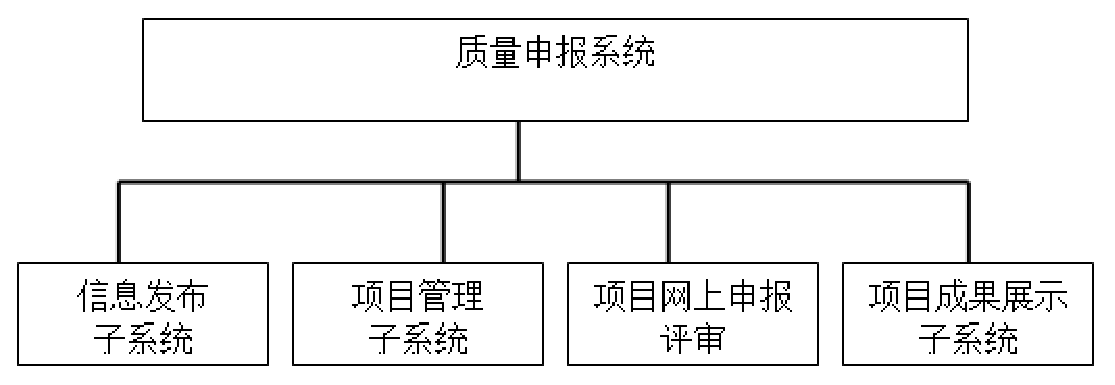
\includegraphics[width=14.6cm]{func_mod}
\caption{系统的主要功能模块}\label{fig:func_mod}
\vspace{\baselineskip}
\end{figure}
图中,各子系统的主要功能简介如下:

(1)	信息发布功能\par
主要是发布项目申报信息、项目指南、建设与改革动态等各类信息。

(2)	项目管理功能\par
主要进行项目分类、项目立项、项目建设过程管理、项目经费管理、项目结题验收管理、项目的统计分析和汇总管理。

(3)	项目的网上申报和网上评审功能\par
网上申报主要提供项目的网上申报功能,提供用户下载与填写申报书和上传申报书。网上评审主要结构专家对用户申报的项目进行评审。

(4)	项目成果展示交流功能\par
主要功能是展示项目的建设成果,并提供专家论坛、交流研讨等交互平台。为用户搭建一个沟通、交流、资源共享的平台。

% !Mode:: "TeX:UTF-8"

\chapter{系统实现技术方法研究}
信息管理系统的实现技术多种多样,所以选择合理的技术来实现系统也是一个重大的环节,如果所选择的技术不当,将对系统的实现造成一定的麻烦,可能还会影响系统的性能。J2EE[7]是实现信息管理系统的一种有效技术,当前用J2EE实现B/S结构的信息管理系统非常的流行且技术也越来越趋于成熟,性能也得到了非常大的提升。轻量级的J2EE应用对于小中型项目的开发带来了许多便利之处,对比于经典J2EE的简化,在保留经典J2EE应用的框架、良好的可扩展性、可维护性的基础上,简化了J2EE应用的开发,降低了J2EE应用的部署成本,基本实现过程简明了。轻量级J2EE应用面向的是用户,是一种更实际的信息化平台架构。

基于Web的J2EE Framework在J2EE的世界内已是空前繁荣,几乎每隔一两个星期就会有新的MVC框架发布。目前比较好的框架中有老牌的Struts、WebWork;新兴的有Spring MVC[9]、Tapestry、JSF等。这些大多是著名团队的作品,另外还有一些边缘团队的作品,也相当出色,如Dinamica、VRaptor等。这些框架都提供了较好的层次分隔能力。在实现良好的MVC分隔的基础上,通过提供一些现成的辅助类库,同时也促进了生产效率的提高。而如何选择一个好的框架应用在项目中,将会对项目的效率与可重用生成重大影响。

实现轻量级J2EE的Spring、Hibernate框架是在各种流行框架之中脱颖而出,逐渐成为软件开发人才,特别是WEB程序开发人才喜爱的开发技术。

本系统的开发拟采用Spring(Spring MVC)、Hibernate框架。以下是框架的简单特征与其在系统开发中的作用。

\section{Spring框架}
服务层的著名开发框架Spring[16]本身就是基于MVC结构的,此外它还具有一些良好的特性,如IOC(或DI)和AOP。Inversion of Control(IOC) 控制反转,就是程序的主控权由应用程序代码本身转移到了框架或容器。Dependency Injection(DI)依赖注入,是一个更能描述其特点的名字,可以解释为容器在运行期将某种依赖关系注入到组件中。

Aspect-Oriented Programming(AOP)面向方面编程通过提供另一种考虑程序结构的方式来补充面向对象编程(OOP)。面向对象将应用程序分解成各个层次的对象,而AOP将程序分解成各个方面或者说关注点。这种方式能够模块化例如事务管理这种横切多个对象的关注点(这种关注点术语称作横切关注点)。AOP框架是Spring的一个关键组件,但Spring IOC容器(Bean Factory)和(Application Context)并不依赖于AOP ,这就意味着如果不需要使用AOP则可不用。AOP补充了Spring IOC ,以提供一个有效的中间件解决方案。[21]

Spring的精简项目的代码量方面做出了非常出色的工作,将大量需要重复书写的代码提取出来,进行切面编程。配置文件的灵活性也使项目的灵活性得到的加强,可以在不改变代码的情况下,而只有改变其中的配置文件实现整个系统的改变。

\section{Spring框架的MVC实现[17]——Spring MVC}
Spring的WEB框架是围绕DispatcherServlet来进行设计的。DispatcherServlet的作用是将请求分发到不同的处理器。图~\ref{fig:req_proc}~展示了DispatcherServlet对请求的处理流程。
\begin{figure}[htbp]
\centering
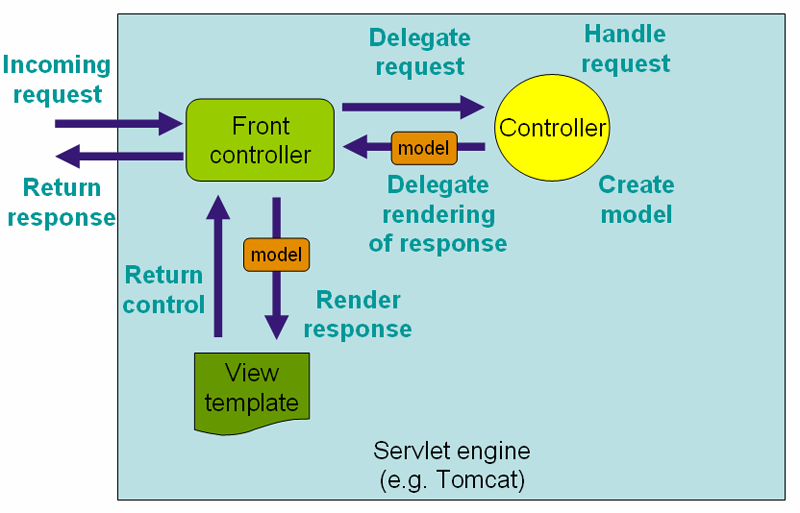
\includegraphics[width=11.65cm]{req_proc}
\caption{Spring Web MVC处理请求工作流程}\label{fig:req_proc}
\vspace{\baselineskip}
\end{figure}
\begin{table}[htbp]
\caption{WebApplicationContext中特殊的bean}\label{tab:bean}
\vspace{0.5em}\centering\wuhao
\begin{tabular}{|m{6cm}|m{6cm}|}
\toprule[1.5pt]
名称 & 描述\\
\midrule[1pt]
控制器(Controller) & 控制器实现的是MVC中Controller那部分\\ \hline
处理器映射(Handler mapping) & 处理器映射包含预处理器(pre-processor),后处理器(post-processor)和控制器的列表,它们在符合某种条件时才被执行(例如符合控制器指定的URL)\\ \hline
视图解析器(View resolvers) & 视图解析器 可以将视图名解析为对应的视图\\ \hline
本地化解析器(Locale resolver) & 本地化解析器能够解析用户正在使用的本地化配置,以提供国际化视图\\ \hline
主题解析器(Theme resolver) & 主题解析器能够解析你的web应用所使用的主题,以提供个性化的布局\\ \hline
上传文件解析器(multipart file resolver) & 上传文件解析器提供HTML表彰文件上传功能\\ \hline
处理异常解析器(Handler exception resolver(s)) & 处理器异常解析器可以将异常对应到视图,或者实现更加复杂的异常处理代码\\
\bottomrule[1.5pt]
\end{tabular}
\vspace{\baselineskip}
\end{table}
DispatcherServlet实际上是一个Servlet,它从HttpServlet继承而来。和其它Servlet一样,DispatcherServlet定义在web应用的web.xml文件中。Spring的Dispatcher有一组特殊的bean,如表~\ref{tab:bean}~所示,用来处理请求和渲染相应的视图。

\section{Hibernate框架}
Hibernate[18]是一种Java语言下的对象关系映射解决方案,它是一种自由、开源的软件。它用来把对象模型表示的对象映射到基于SQL的关系模型结构中去,为面向对象的领域模型到传统的关系型数据库的映射,提供了一个使用方便的框架。Hibernate不仅管理Java类到数据库表的映射(包括从Java数据类型到SQL数据类型的映射),还提供数据查询和获取数据的方法,可以大幅度减少开发时人工使用SQL和JDBC处理数据的时间。它的设计目标是将软件开发人员从大量相同的数据持久层相关编程工作中解放出来。无论是从设计草案还是从一个遗留数据库开始,开发人员都可以采用Hibernate。

下面从Hibernate的体系结构与Hibernate API两方面对Hibernate进行介绍。

(1) hibernate体系结构简介
\begin{figure}[htbp]
\centering
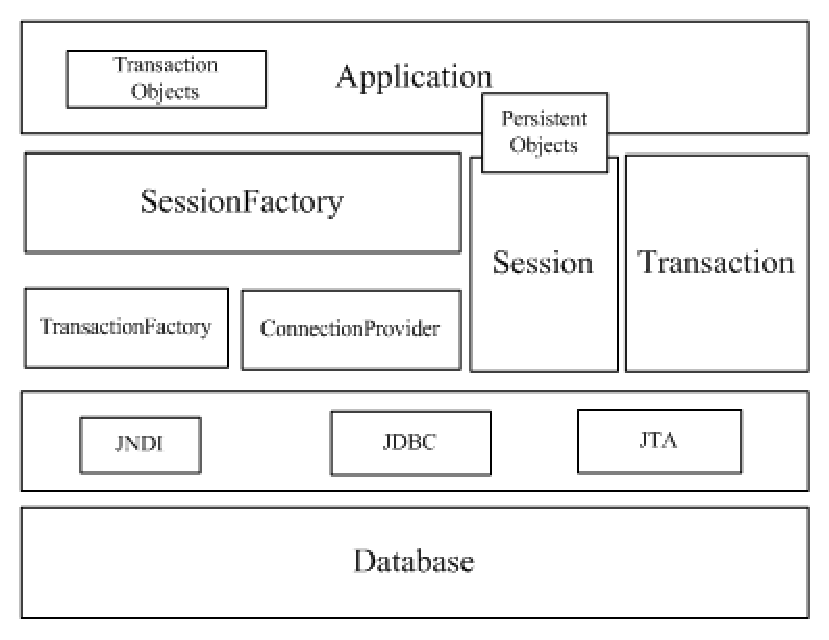
\includegraphics[width=10.01cm]{arch}
\caption{Hibernate体系结构图}\label{fig:arch}
\vspace{\baselineskip}
\end{figure}
图~\ref{fig:arch}~各对象的说明如下:\par
SessionFactory:针对单个数据库映射关系经过编译后的内在镜像,是线程安全的,它是生成Session的工厂。\par
Session:表示应用程序与持久存储层之间交互操作的一个单纯种对象,此对象生存期很短。其隐藏了JDBC连接,也是Transaction的工厂。\par
持久对象及集合:带有持久化状态的、具有业务功能的单线程对象,此对象生存期很短。这些对象可能是普通的JavaBeans/POJO,唯一特殊的是他们正与(仅仅一个)Session相关联。一旦这个Session被关闭,这些对象就会脱离持久化状态,这样就可被应用程序的任何层自由使用。\par
瞬态(transient)和脱管(detached)的对象及其集合:那些目前没有与session关联的持久化类实例。他们可能是在被应用程序实例化后,尚未进行持久化的对象,也可能是因为实例化他们的Session已经被关闭而脱离持久化的对象。\par
事务Transaction:应用程序用来指定原子操作单元范围的对象,它是单线程了,生命周期很短。\par
Hibernate作为模型/数据访问层。它通过配置文件(hiberante.cfg.xml或hibernate.properties和映射文件(*.hbm.xml)把java对象或持久化对象(Persistent Obeject,PO)映射到数据库中的数据表,然后通过操作PO,对数据库中的表进行各种操作。

(2) Hibernate API简介\par
Hibernate API中的接口可分为以下几类:\par
(a)	提供访问数据库的操作的接口,包括Session、Transaction、Query接口。\par
(b)	用于配置Hibernate的接口,Configuration(如下在Spring应用中,将由Spring来完成Hibernate的相关配置)。\par
(c)	间接接口,使应用程序接受Hibernate内部发生的事件,并作出相应的回应,包括:Interceptor、LifeCycle、Validatable。\par
(d)	用户于扩展Hibernate功能的接口,如UserType、CompositeUserType接口。\par
Hibernate内部还封装了JDBC、JTA(Java Transaction API)和JNDI(Java Naming And Directory Interface)。其中,JDBC提供底层的数据访问操作,只要用户提供了相应的JDBC驱动程序,Hibernate可以访问任何一个数据库系统。JTA和JNDI使Hibernate能够和J2EE应用服务器集成。具体接口间的协作如图~\ref{fig:interface}~所示。 
\begin{figure}[htbp]
\centering
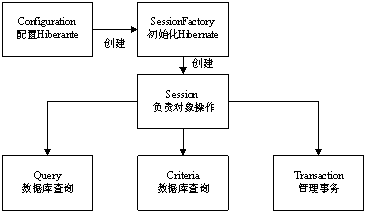
\includegraphics[width=11.1cm]{interface}
\caption{Hibernate核心接口}\label{fig:interface}
\vspace{\baselineskip}
\end{figure}

\section{AJAX技术}
AJAX[21]全称为“Asynchronous JavaScript and XML”(异步JavaScript和XML),是指一种创建交互式网页应用的网页开发技术。主要包含了以下几点技术:基于web标准(standards-based presentation)XHTML+CSS的表示;使用DOM(Document Object Model)进行动态显示及交互;使用XML和XSLT进行数据交换及相关操作;使用XMLHttpRequest进行异步数据查询、检索;使用JavaScript[22]将所有的东西绑定在一起。类似于DHTML或LAMP,AJAX不是指一种单一的技术,而是有机地利用了一系列相关的技术。使用Ajax的最大优点,就是能在不更新整个页面的前提下维护数据,这使得Web应用程序更为迅捷地回应用户动作,并避免了在网络上发送那些没有改变过的信息[23]。

\section{框架之间的有机整合}
Spring与Hibernate的集成是通过配置完成的。通过一个个的配置文件实现两者框架之间的连接。

Hibernate与Spring的集成。Spring 为持久层的开发提供了强有力的支持,其中对于Hibernate 的支持包括HibernateTemplate , HibernateInterceptor 和Hibernate transaction manager 。Hibernate 的连接、事务管理等是由SessionFactory 开始的,SessionFactory底层的DataSource 可以使用Spring 的IOC 注入,然后将SessionFactory 注入到相应的对象中。

% !Mode:: "TeX:UTF-8"

\chapter{总结与展望}
随着我国高等教育规模的不断扩大,教学质量的不断提高,研究项目的不断增多,信息化程不断增高,基于互联网的项目申报系统将日益受到重视[27]。传统的纸质项目申报评审方式面临着很大的挑战,迫切要求我们实现项目申报评审的科学化、现代化。对此,网上项目申报评审系统的开发日益迫切,项目的开发意义也越来越重要。

	“浙江省教育厅教育质量与教学改革项目申报管理系统”是一个集项目信息发布、项目管理、项目网上申报评审管和项目成果展示为一体的信息化管理系统。为用户提供一个方便、快捷、透明、高效的项目申报评审环境。系统的实现将有效的提高项目主管部门、学校、老师的工作效率,带来巨大的经济效益。


\endgroup % 组结束
%%%%%%%%%% 参考文献 %%%%%%%%%%
\clearpage % 显式换页,使书签定位准确
\defaultfont
\bibliographystyle{GBT7714-2005NLang-ZJUT}
\phantomsection
\markboth{参考文献}{参考文献}
\addcontentsline{toc}{chapter}{参考文献}       % 参考文献加入到中文目录
\nocite{*}                                     % 若将此命令屏蔽掉,则未引用的文献不会出现在文后的参考文献中。
\bibliography{references/reference}

\end{document}
